\chapter{Experiments}\label{chap:experiments}

In this chapter we are going to present the experimental results. We focus hereby on two main sections: ``Training Latent Models'' and ``Reinforcement Learning''. In the first section we will cover all results on training Latent Models including experiments with the Variational Autoencoder and Supervised model trained with different loss functions as introduced in \chapref{chap:Methodology}. \\
The second section ``Reinforcement Learning'' is going to present the results on how the Soft Actor-Critic handles the introduced 2D inverse kinematics environment and how the fusion with the pre-trained latent models affects the training


\section{Training of Latent Models}

In this section we will present the results on the conducted experiments how to train a Variational Autoencoder and supervised model. We train both models with two distinct loss functions: The distance loss and a weighted sum of the distance loss and imitation loss. 

\subsection{Variational Autoencoder}

In the following section we will present the results of our experiments with the Variational-Autoencoder to encode and decode actions from the environment but also learn to solve inverse kinematics by minimizing the presented distance loss form \eqref{eqn:Distance-Loss}. Within the section we are covering two loss function setups. The first setup we are going to concentrate on only uses the distance loss while the second setup incorporates also an imitation loss.

\subsubsection{Distance Loss}

Coming up are the training results for different latent dimensions but only with the distance loss enabled which means \texttt{dataset target mode = POSITION}.\\ 
Because we only leverage the usage of the distance loss we do not need to encode and decode an action from an inverse kinematics solver, we just need to encode target information where we want to go plus state information as conditional information.
\begin{figure}
    \begin{center}
        \subfloat[mean reconstruction loss over the las 20 epochs for \textbf{latent dimension = 2}]{
            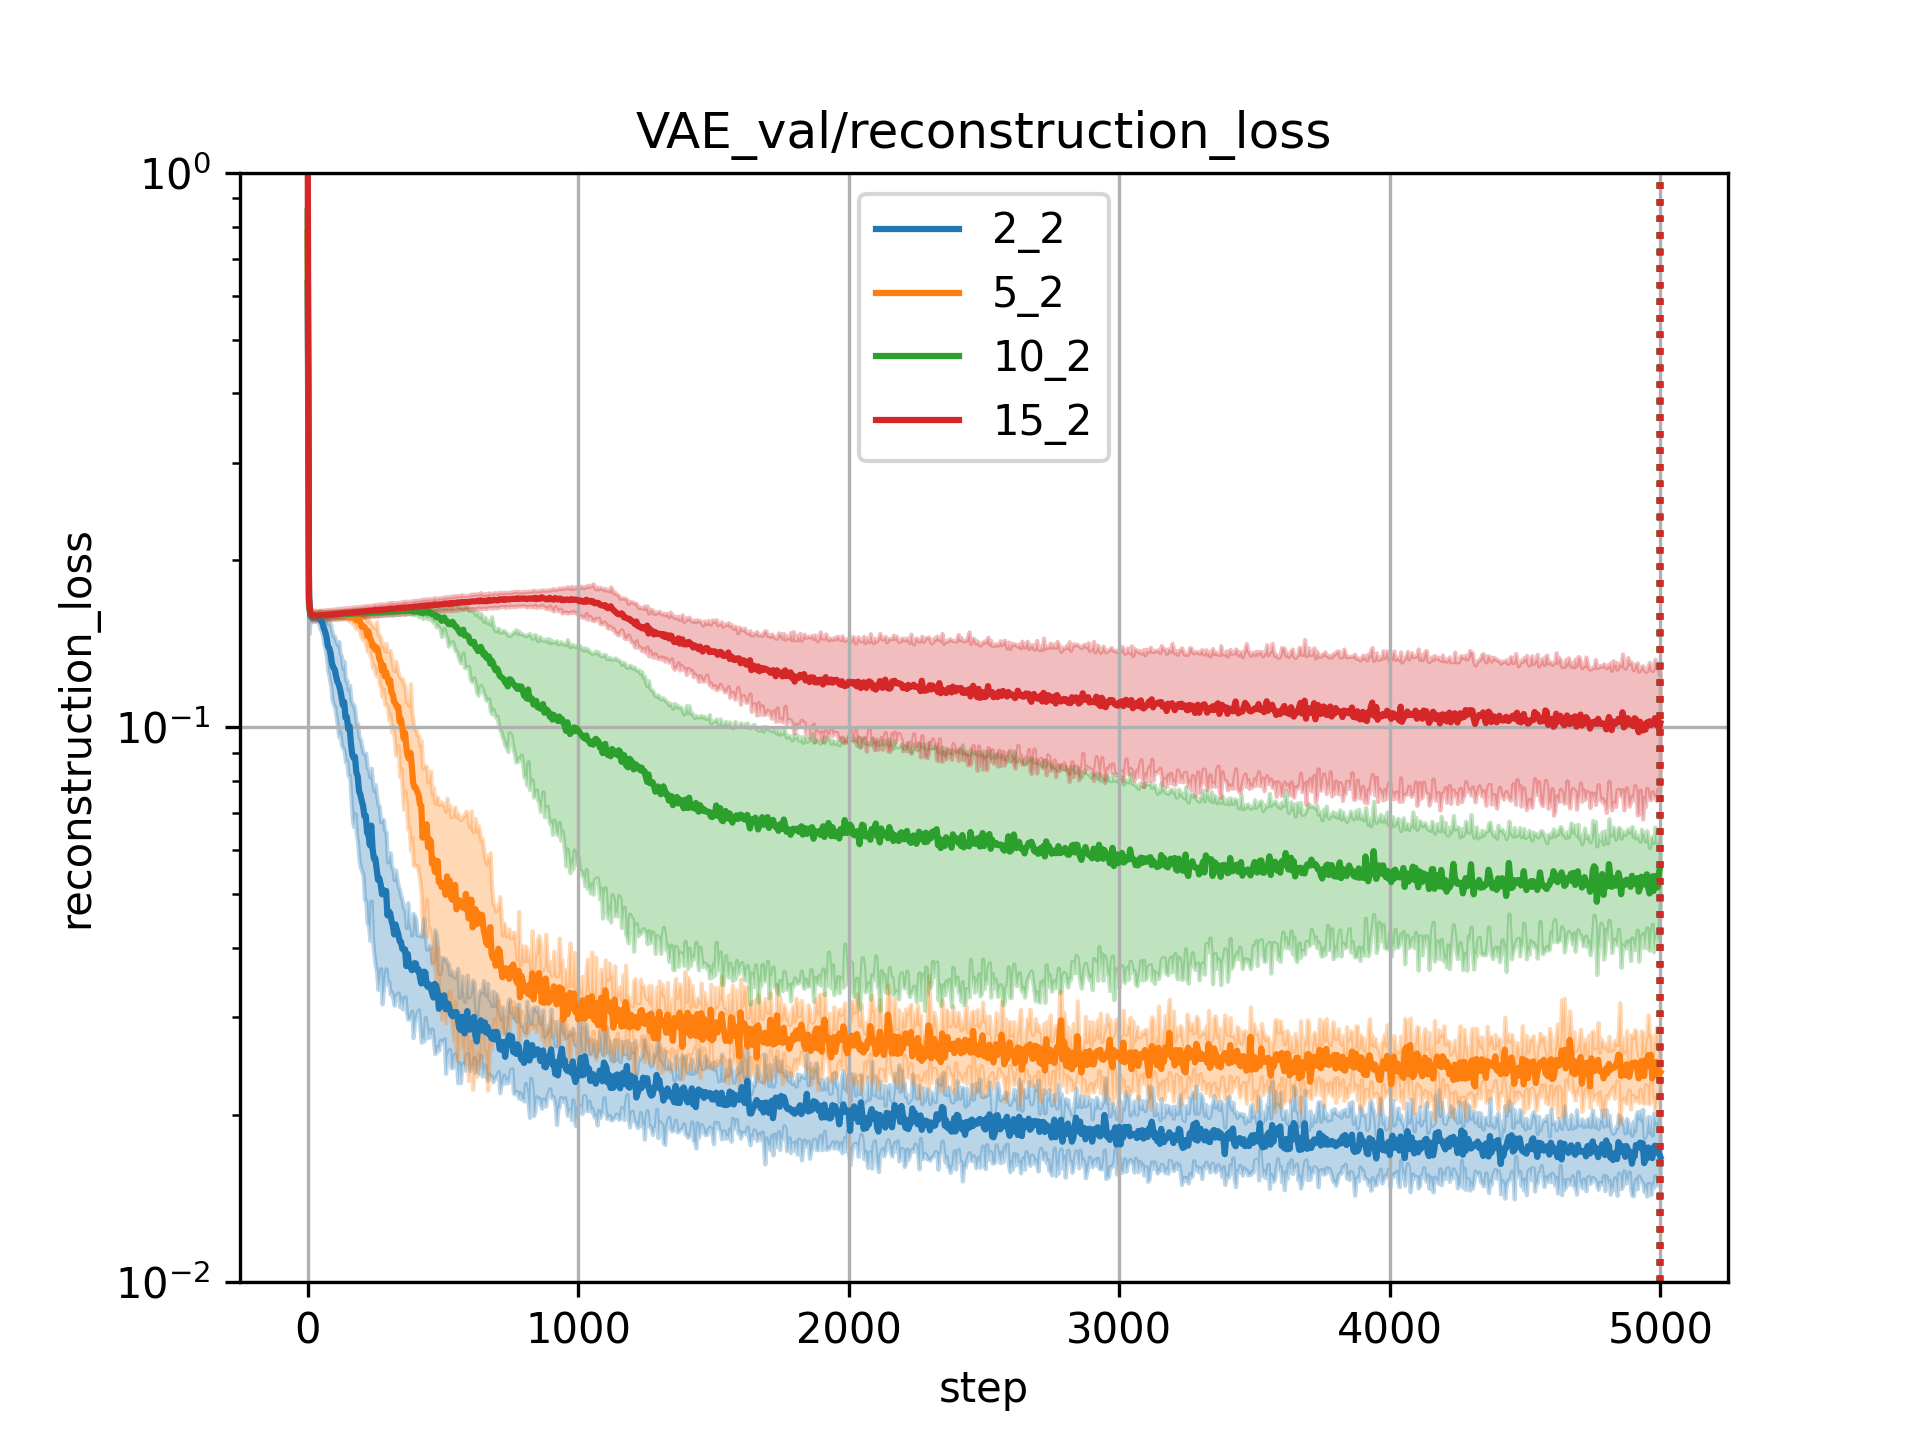
\includegraphics[width=0.31 \linewidth]{figures/experiments/vae_comparison_latent_2_reconstruction_loss.png}
            \label{fig:VAE_latent/reconstruction_2}
            }
        \hfill
        \subfloat[mean reconstruction loss over the las 20 epochs for \textbf{latent dimension = 4}]{
            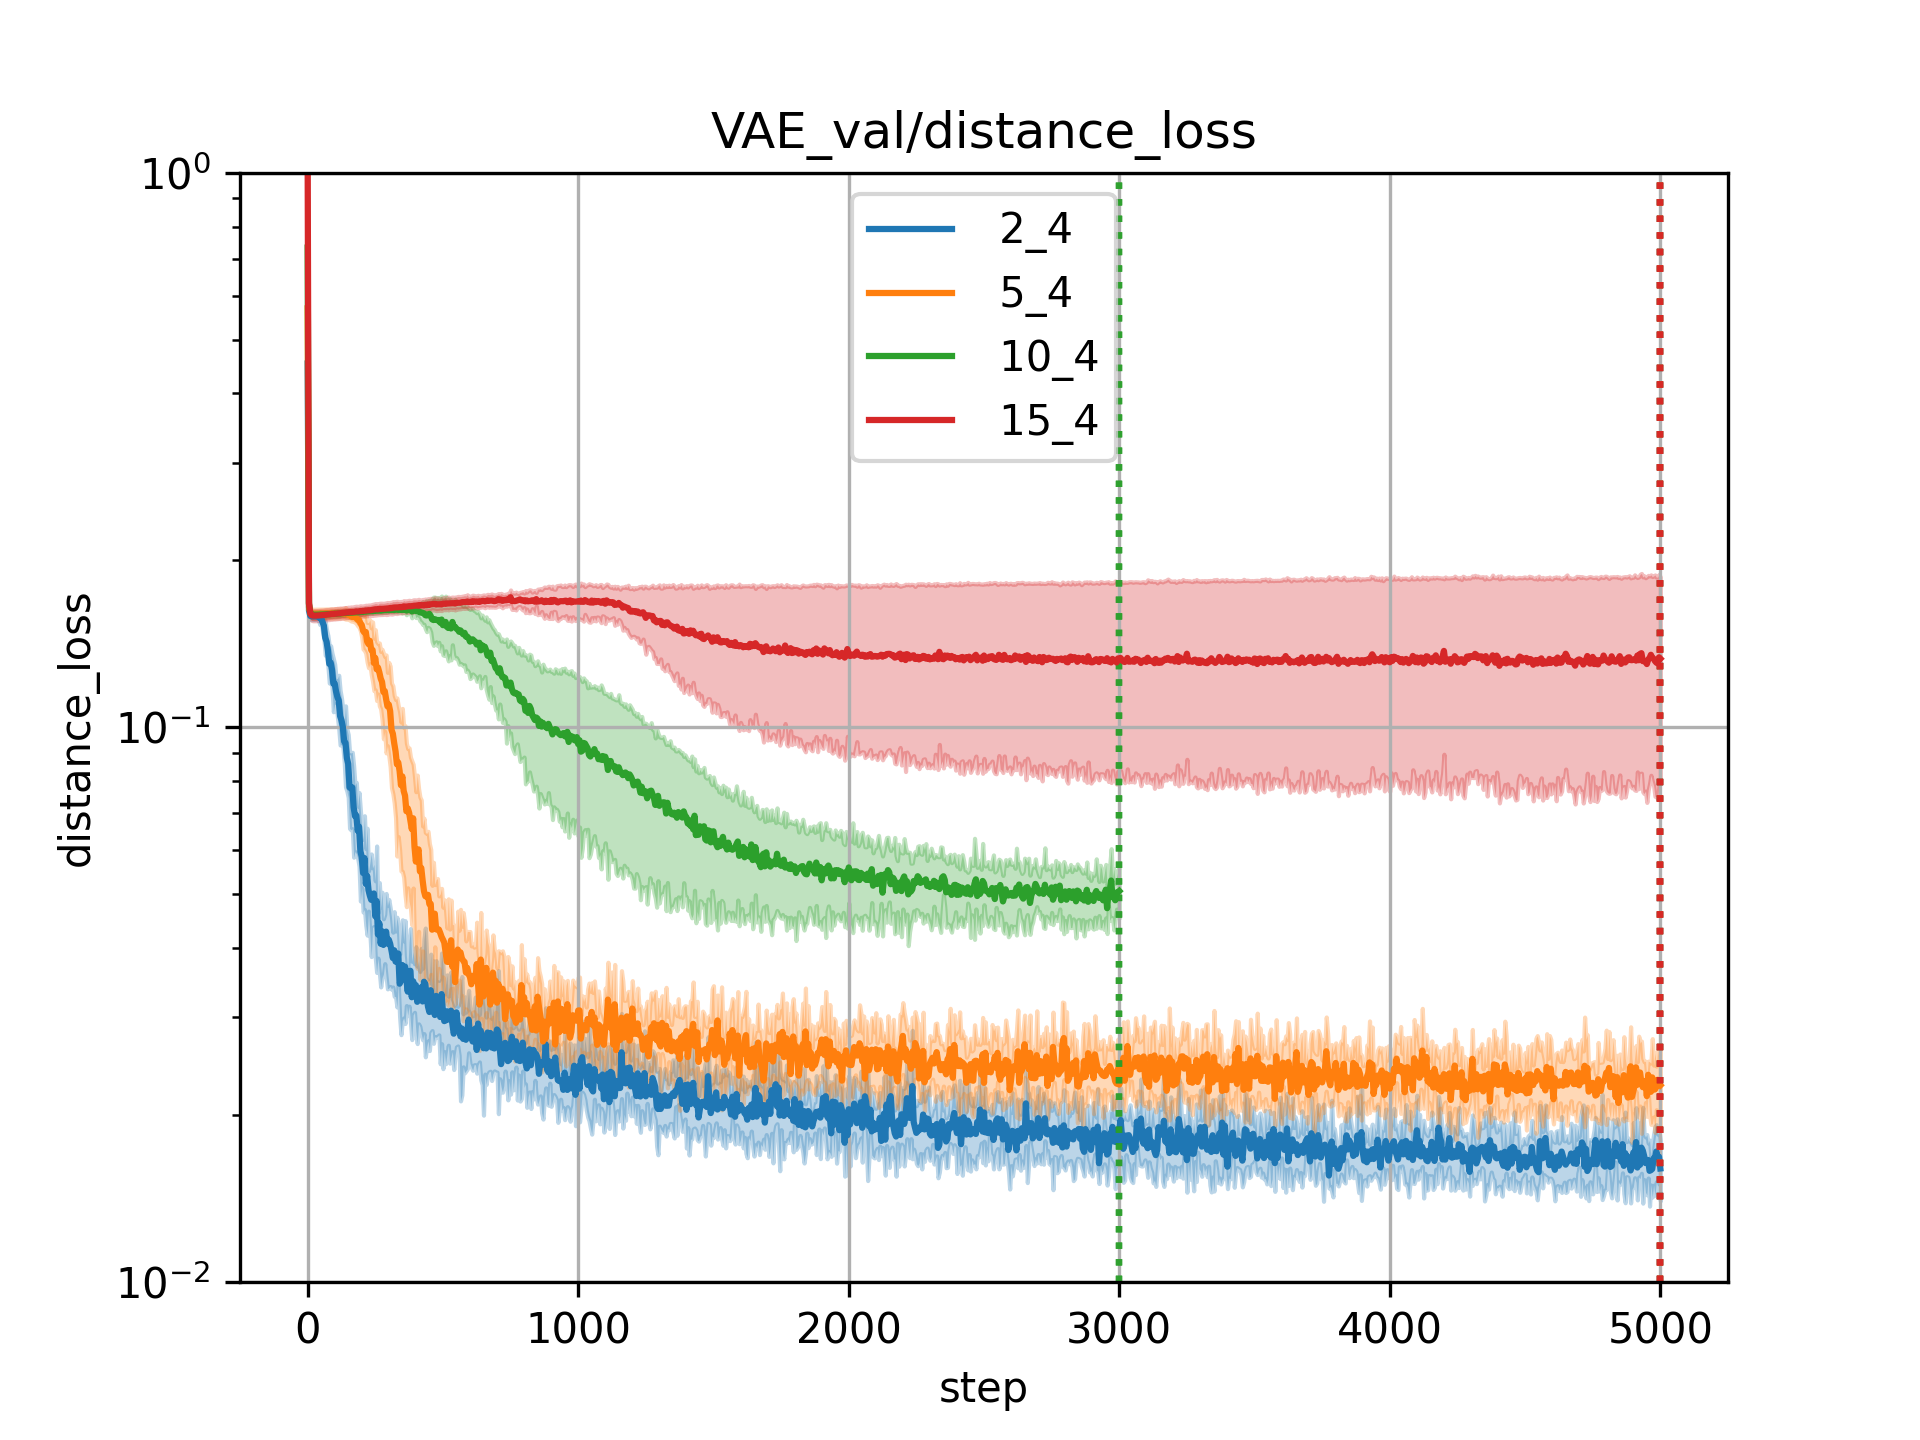
\includegraphics[width=0.31 \linewidth]{figures/experiments/vae_comparison_latent_4_reconstruction_loss.png}
            \label{fig:VAE_latent/reconstruction_4}
            }
        \hfill
        \subfloat[mean reconstruction loss over the las 20 epochs for \textbf{latent dimension = 8}]{
            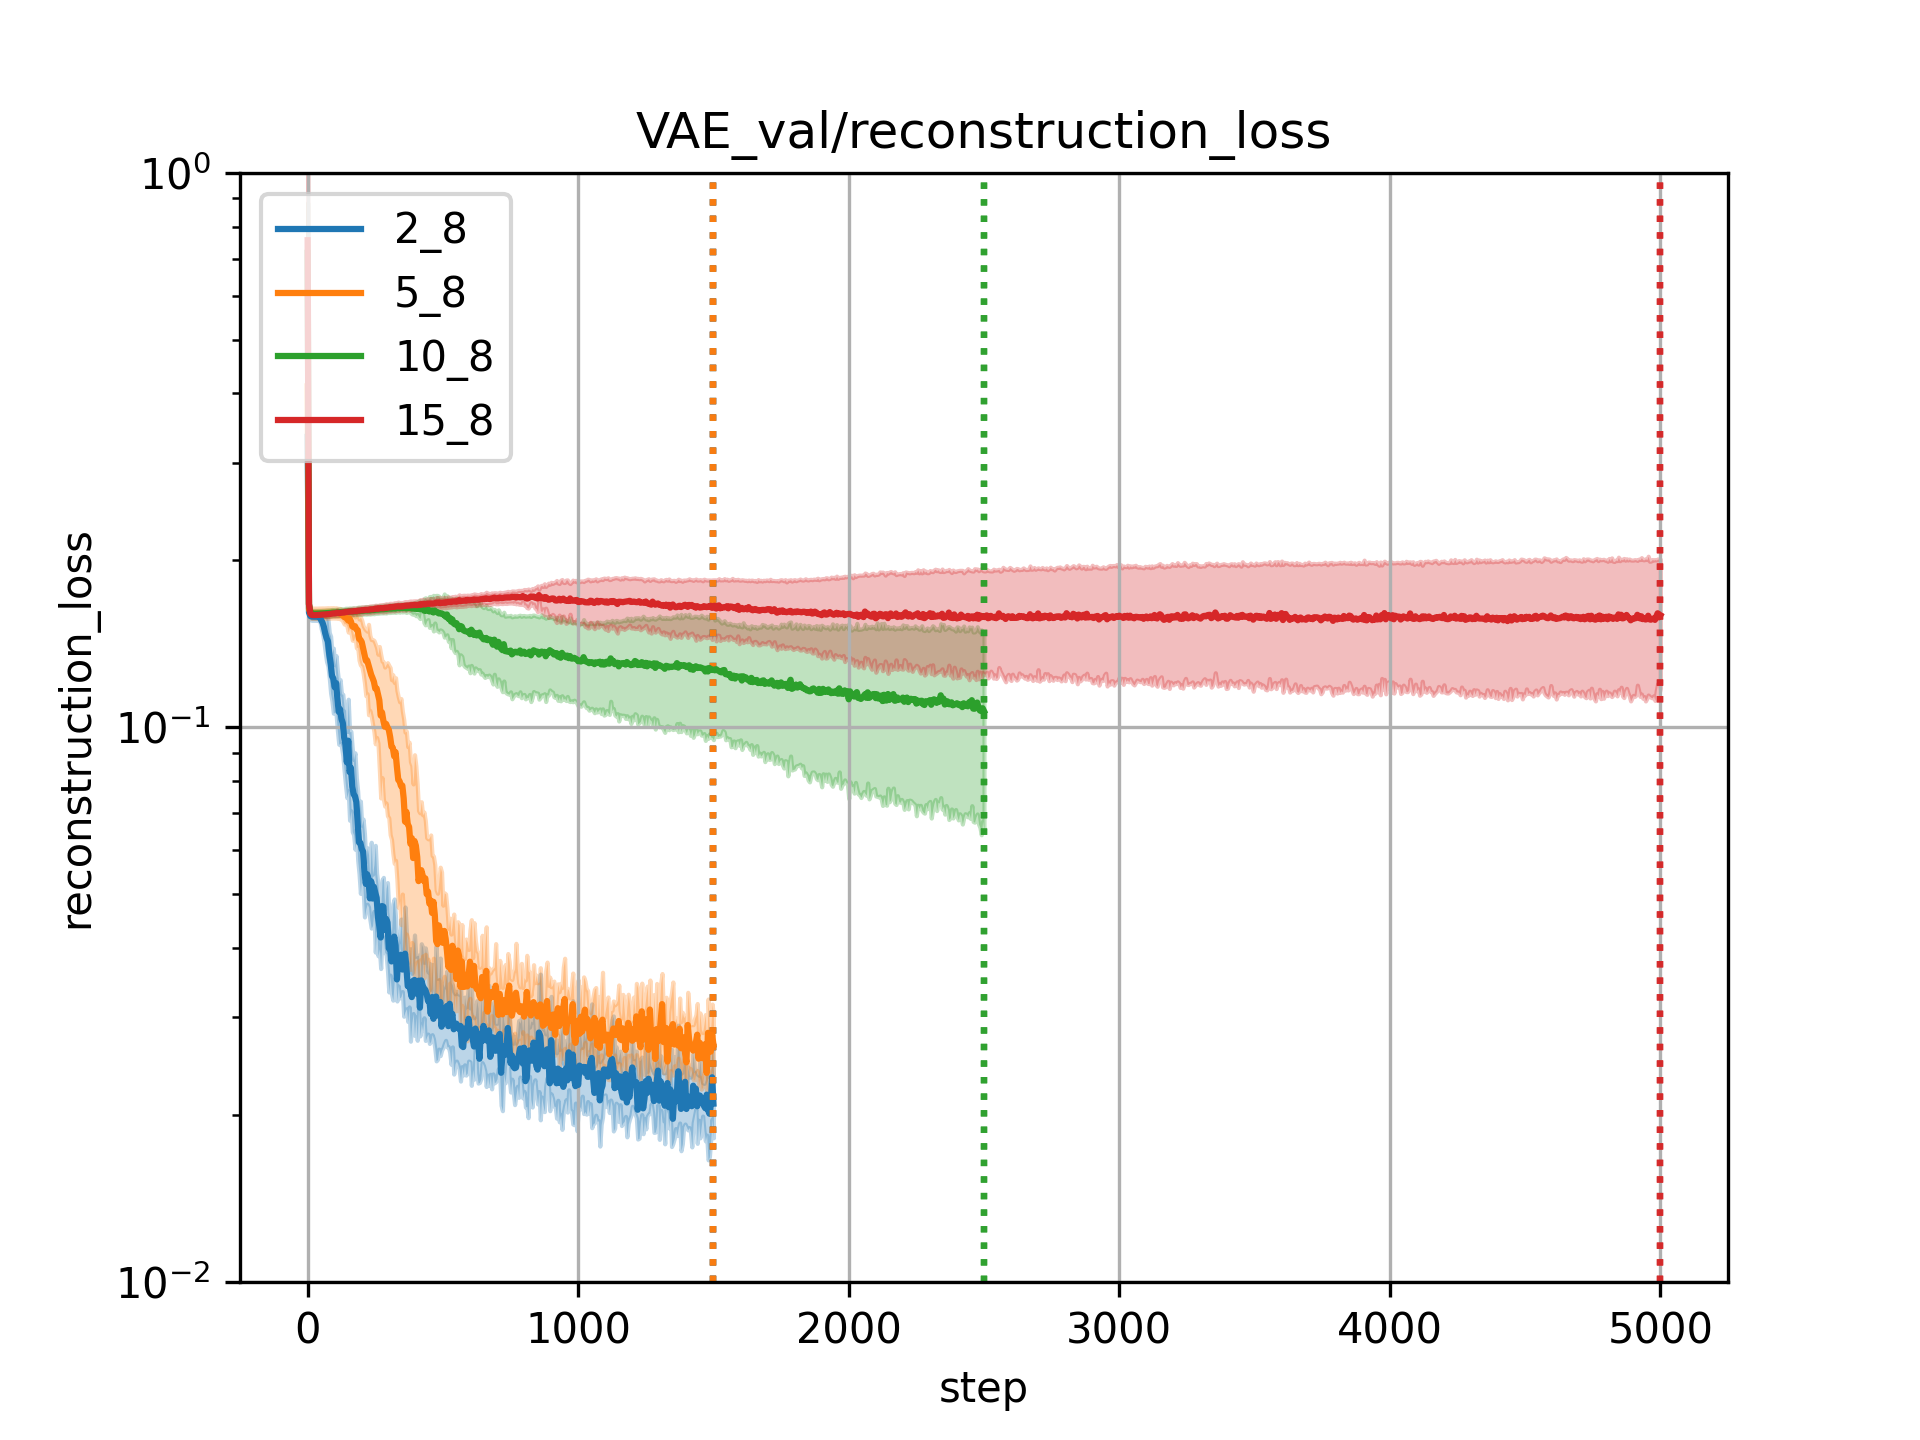
\includegraphics[width=0.31 \linewidth]{figures/experiments/vae_comparison_latent_8_reconstruction_loss.png}
            \label{fig:VAE_latent/reconstruction_8}
            }
        \\
        \subfloat[mean KL-loss over the las 20 epochs for \textbf{latent dimension = 2}]{
        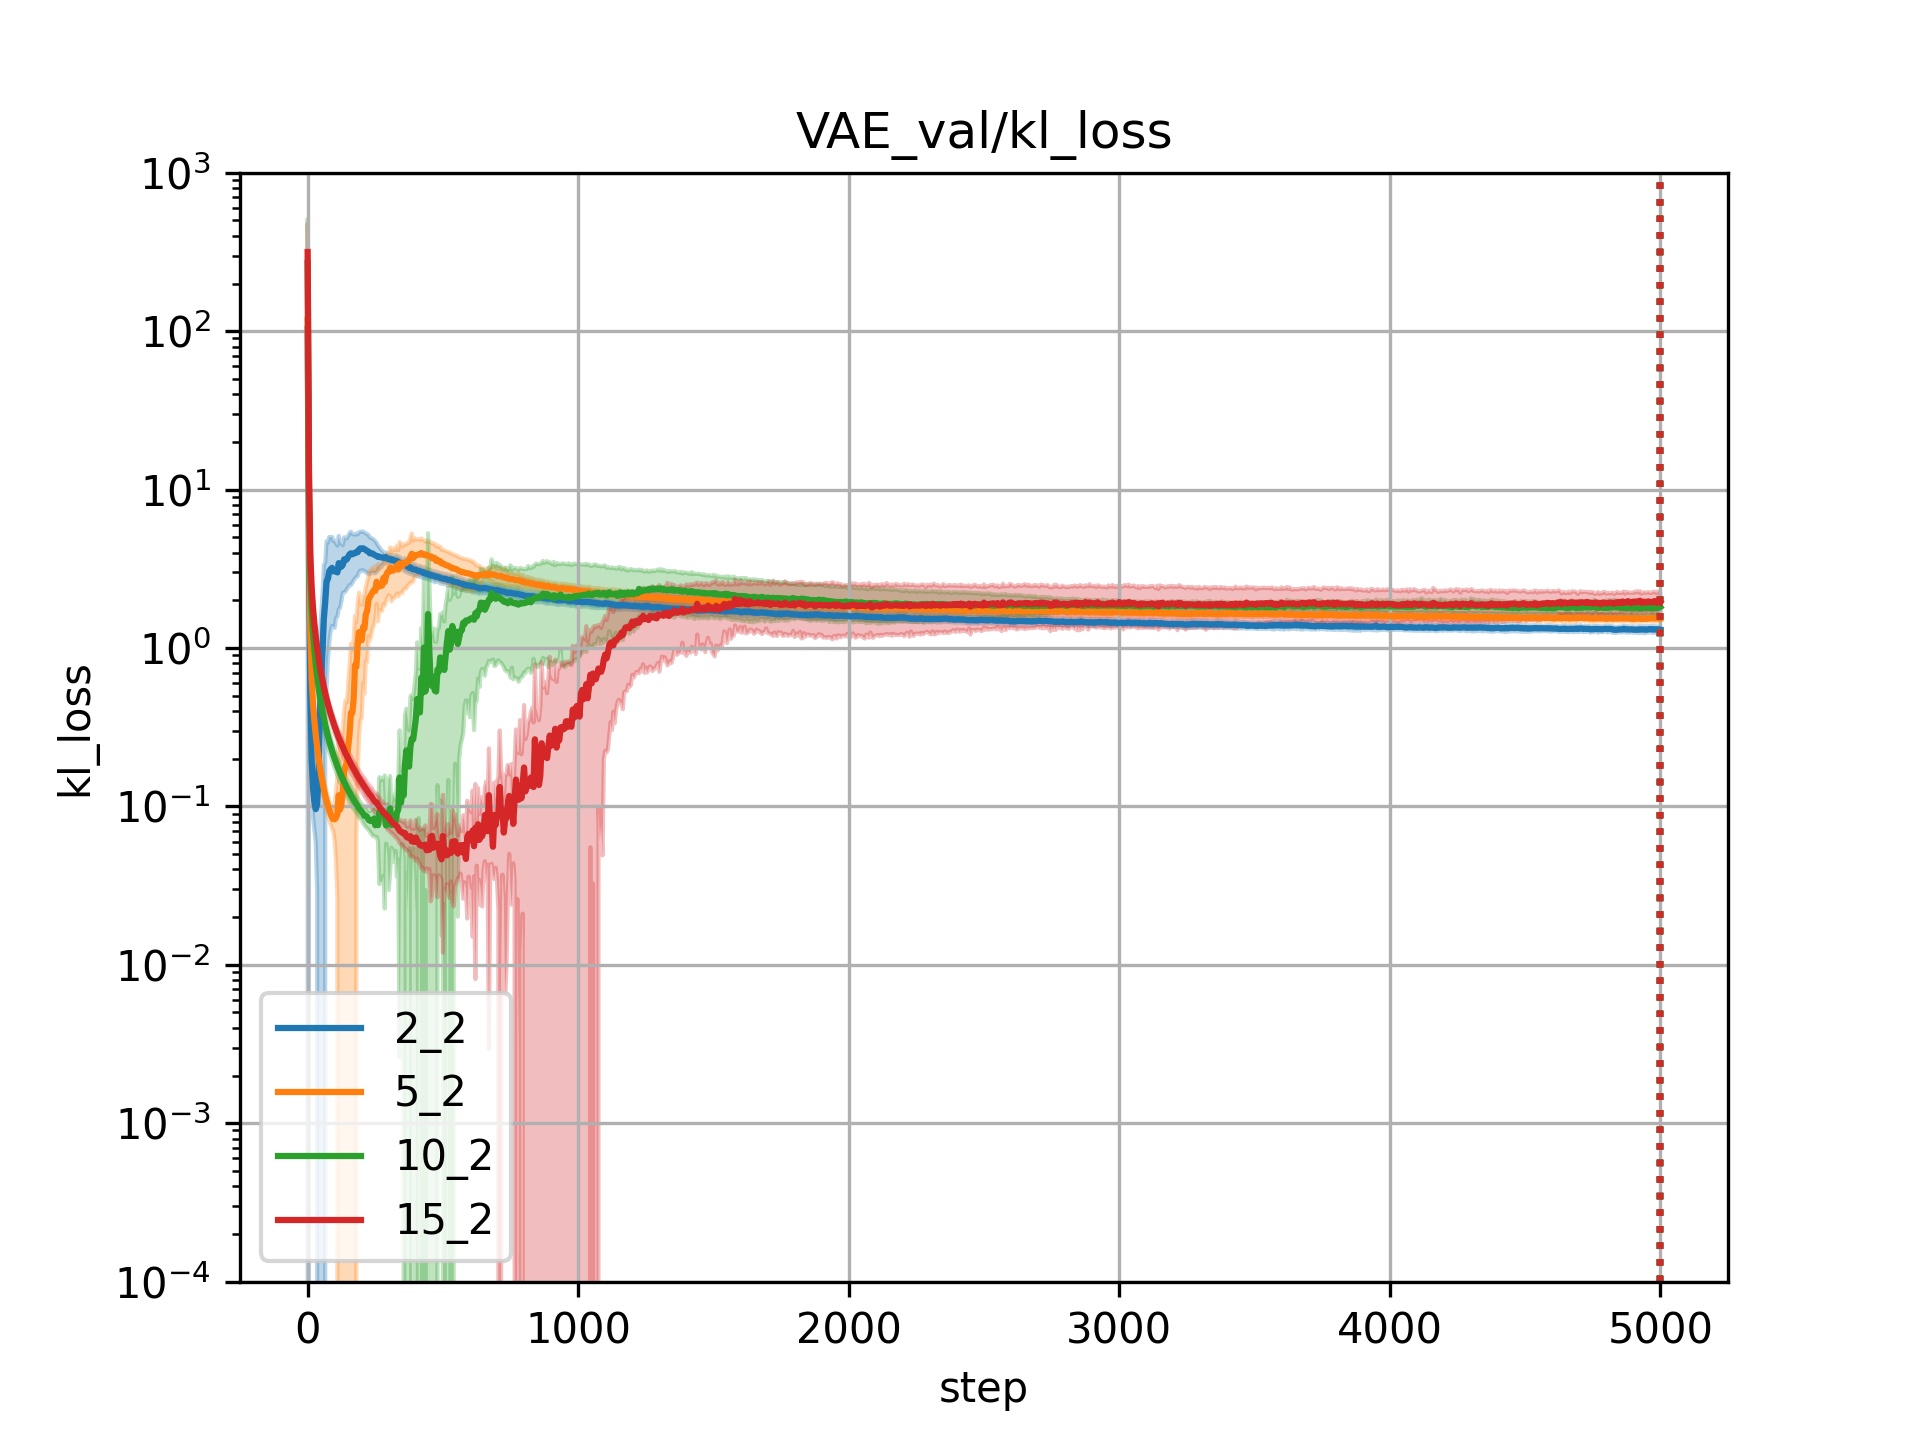
\includegraphics[width=0.31 \linewidth]{figures/experiments/vae_comparison_latent_2_kl_loss.png}
            \label{fig:VAE_latent/kl_2}
            }
        \hfill
        \subfloat[mean KL-loss over the las 20 epochs for \textbf{latent dimension = 4}]{
        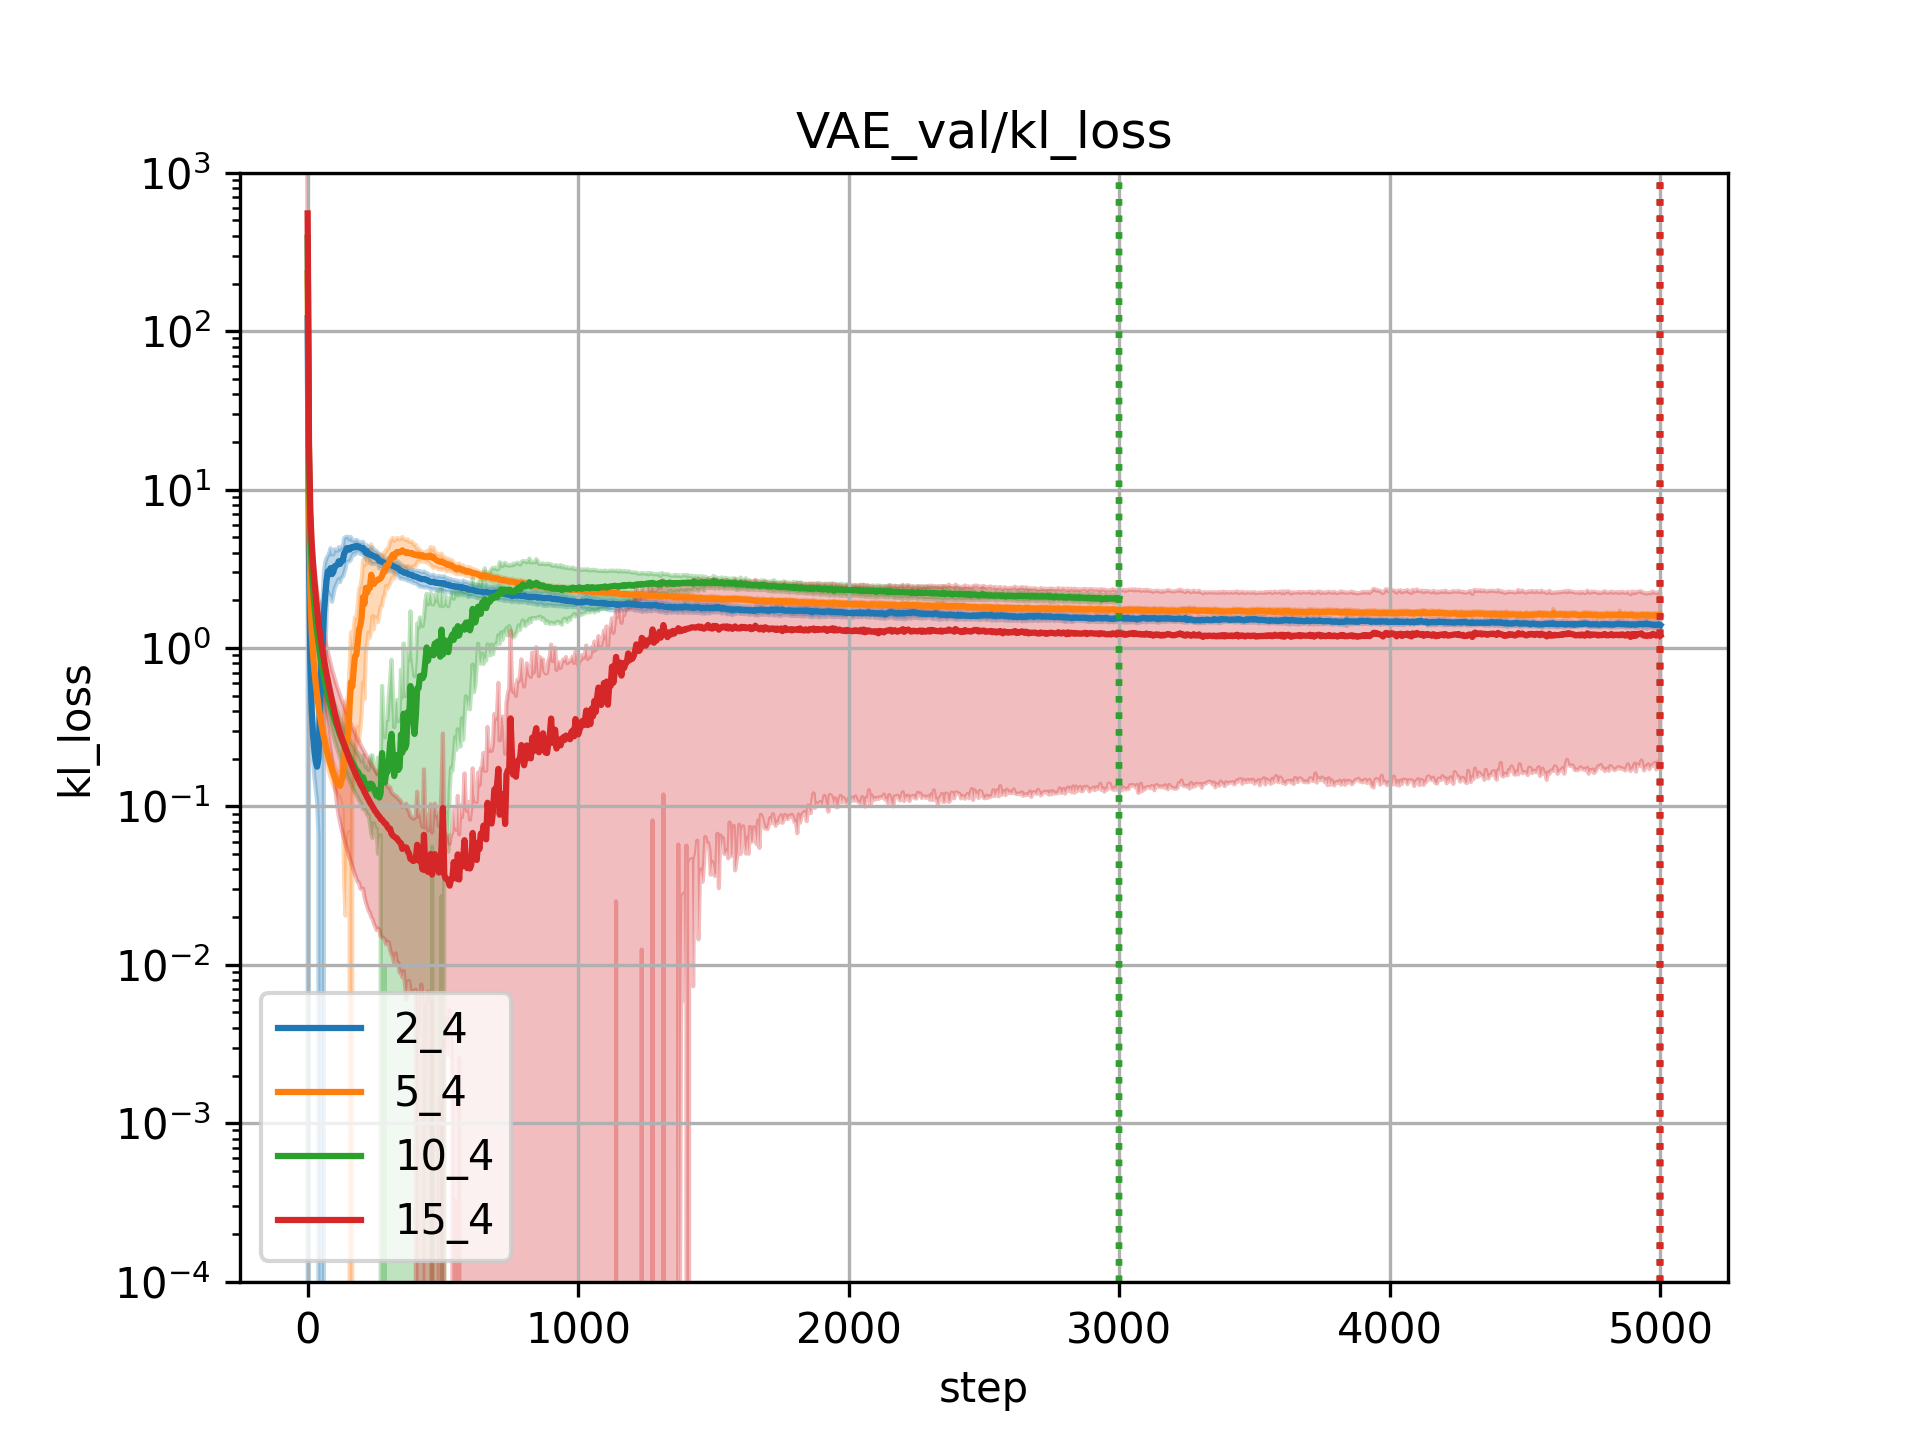
\includegraphics[width=0.31 \linewidth]{figures/experiments/vae_comparison_latent_4_kl_loss.png}
            \label{fig:VAE_latent/kl_4}
            }
        \hfill
        \subfloat[mean KL-loss over the las 20 epochs for \textbf{latent dimension = 8}]{
        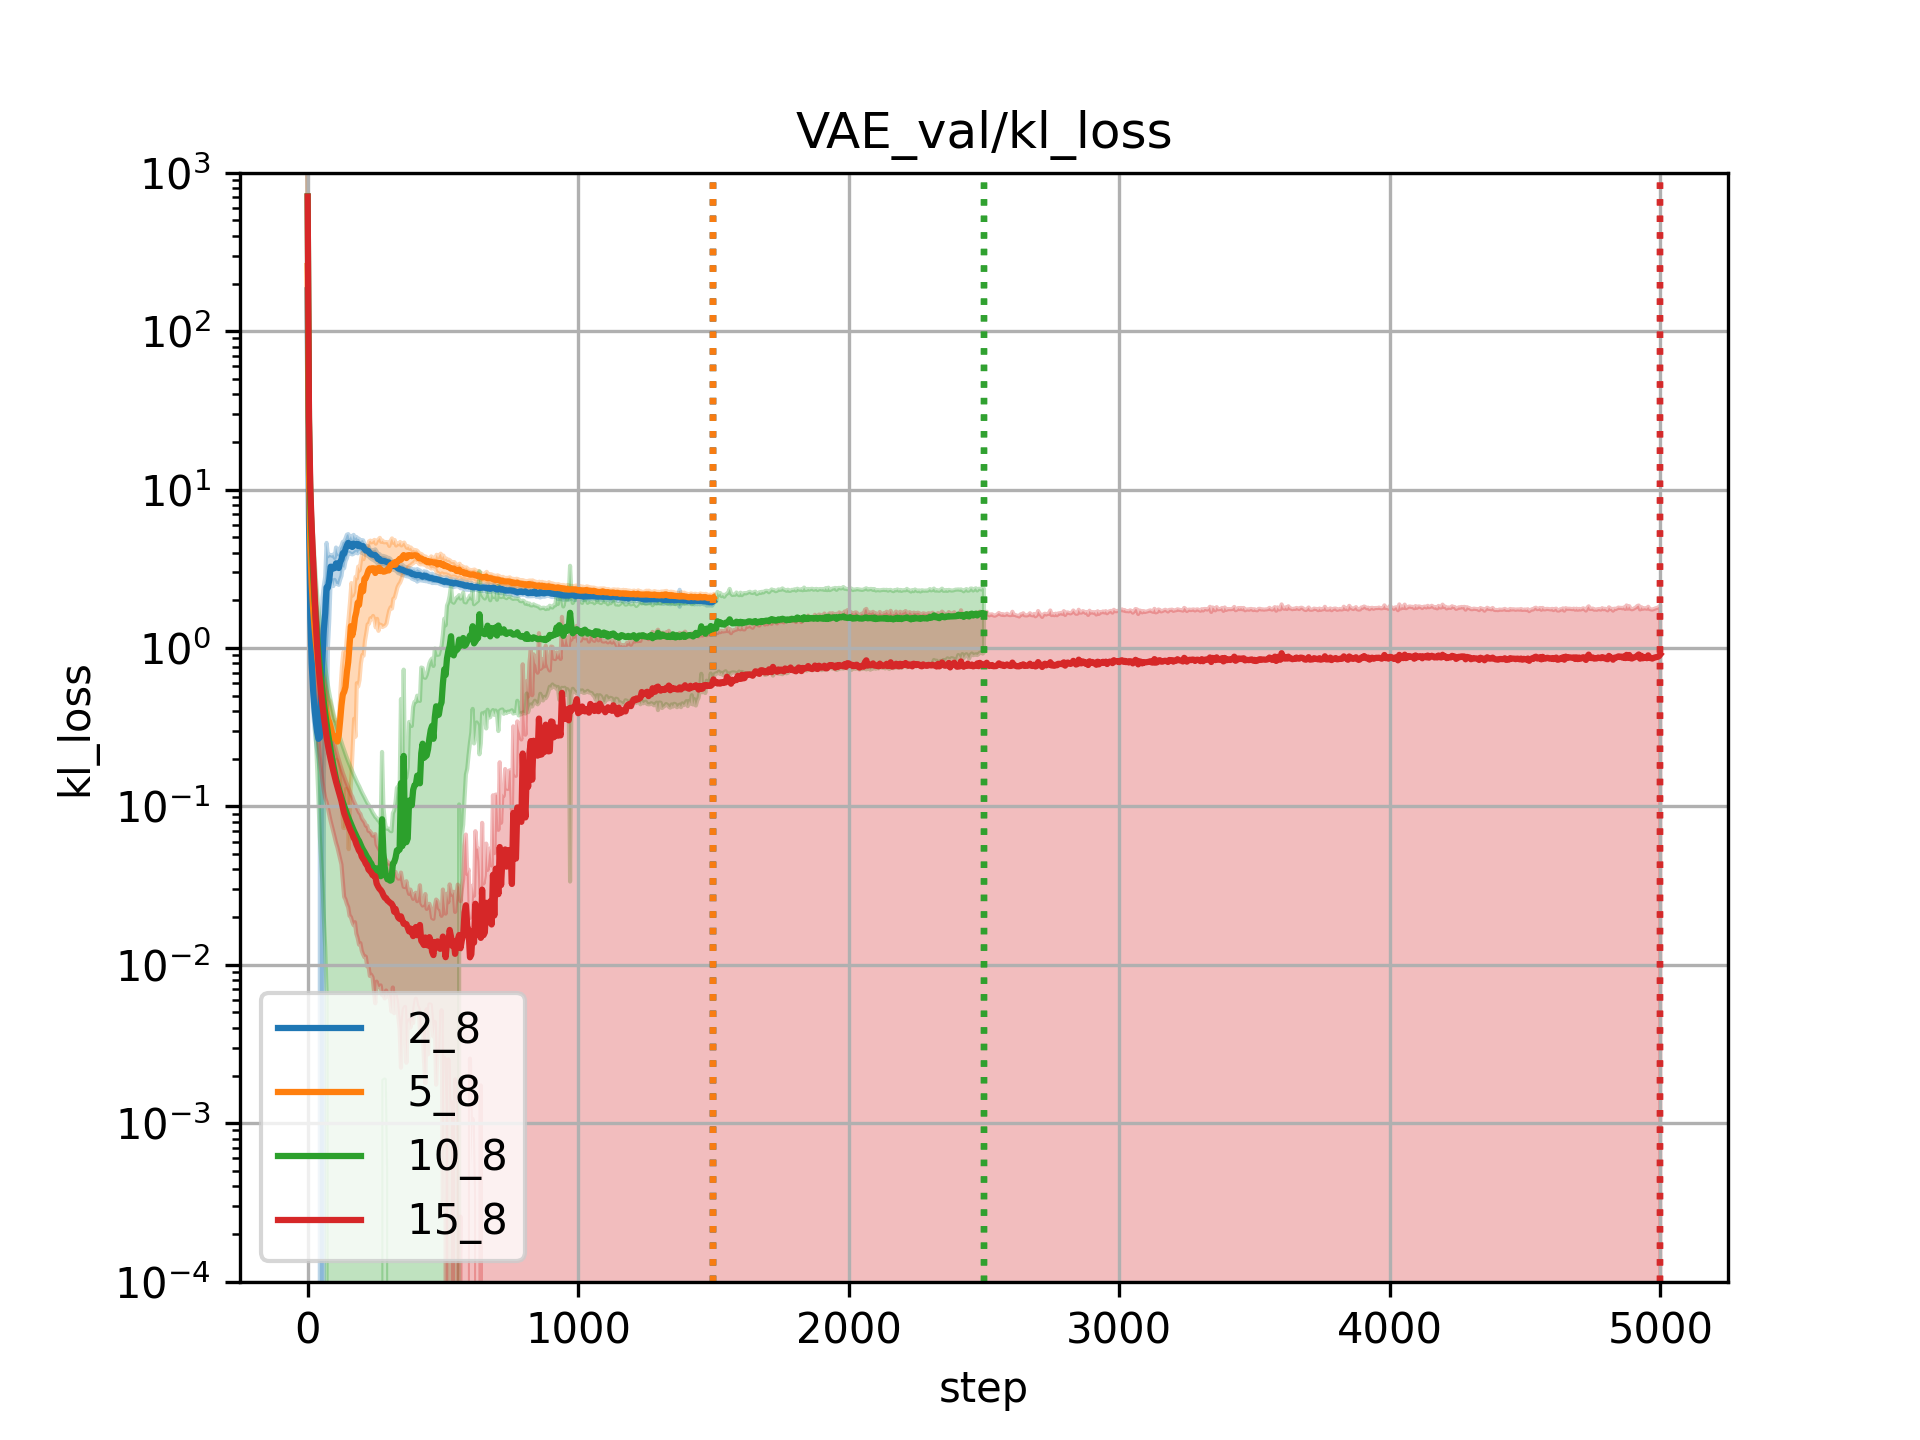
\includegraphics[width=0.31 \linewidth]{figures/experiments/vae_comparison_latent_8_kl_loss.png}
            \label{fig:VAE_latent/kl_8}
            }
    \end{center}
    \caption[VAE validation results, only distance loss and latent = 4]{VAE validation results over different amounts of joints and with a latent dimension of 4. Each experiment was conducted 10 times with different random seeds. The solid curve is the average over those 10 experiments and the color shaded area resembles the standard deviation. Notice that the y axis in bot plots is in log scale.}
    \label{fig:VAE_latent}
\end{figure}

In \figref{fig:VAE_latent} we have a closer look into the reconstruction loss and kl loss. While increasing the number of joints $N \in [2, 5, 10, 15]$ we are also increasing the level of complexity the network has to master to come up with suitable action which leads to a low distance loss. The increasing level of complexity is quite noticeable in both the kl loss and reconstruction loss. \\
All KL-Loss curves in \figref{fig:VAE_latent} (d) to (e) are shaped in the same way. First a drop before rising with a little overshoot and finally approaching the terminal value asymptotically. While increasing $N$ we can see that the first local minimum shifts to the right, the upwards slope becomes slacker and the overshoot diminishes. This behavior confirms the the theory of increasing complexity while increasing the number of joints.\\
We can find another indicator by analyzing the reconstruction loss in \figref{fig:VAE_latent} (a) to (c). For all joints it is quite clear that the learning curves are shaped similar but approaching different final performances. For those experiments of $N \in [2, 5]$ we get a reconstruction loss $< 0.02$ independent of the latent dimension. But if we turn towards $N = 10$ we can clearly see that the latent dimension does make a significant difference between finding a solution, with a latent dimension of four, or failing with a latent dimension of eight. A further increase of $N$ does not lead to better reconstruction losses across all latent space dimensions. 
\begin{figure}
    \begin{center}
        \subfloat[$N = 2$]{
            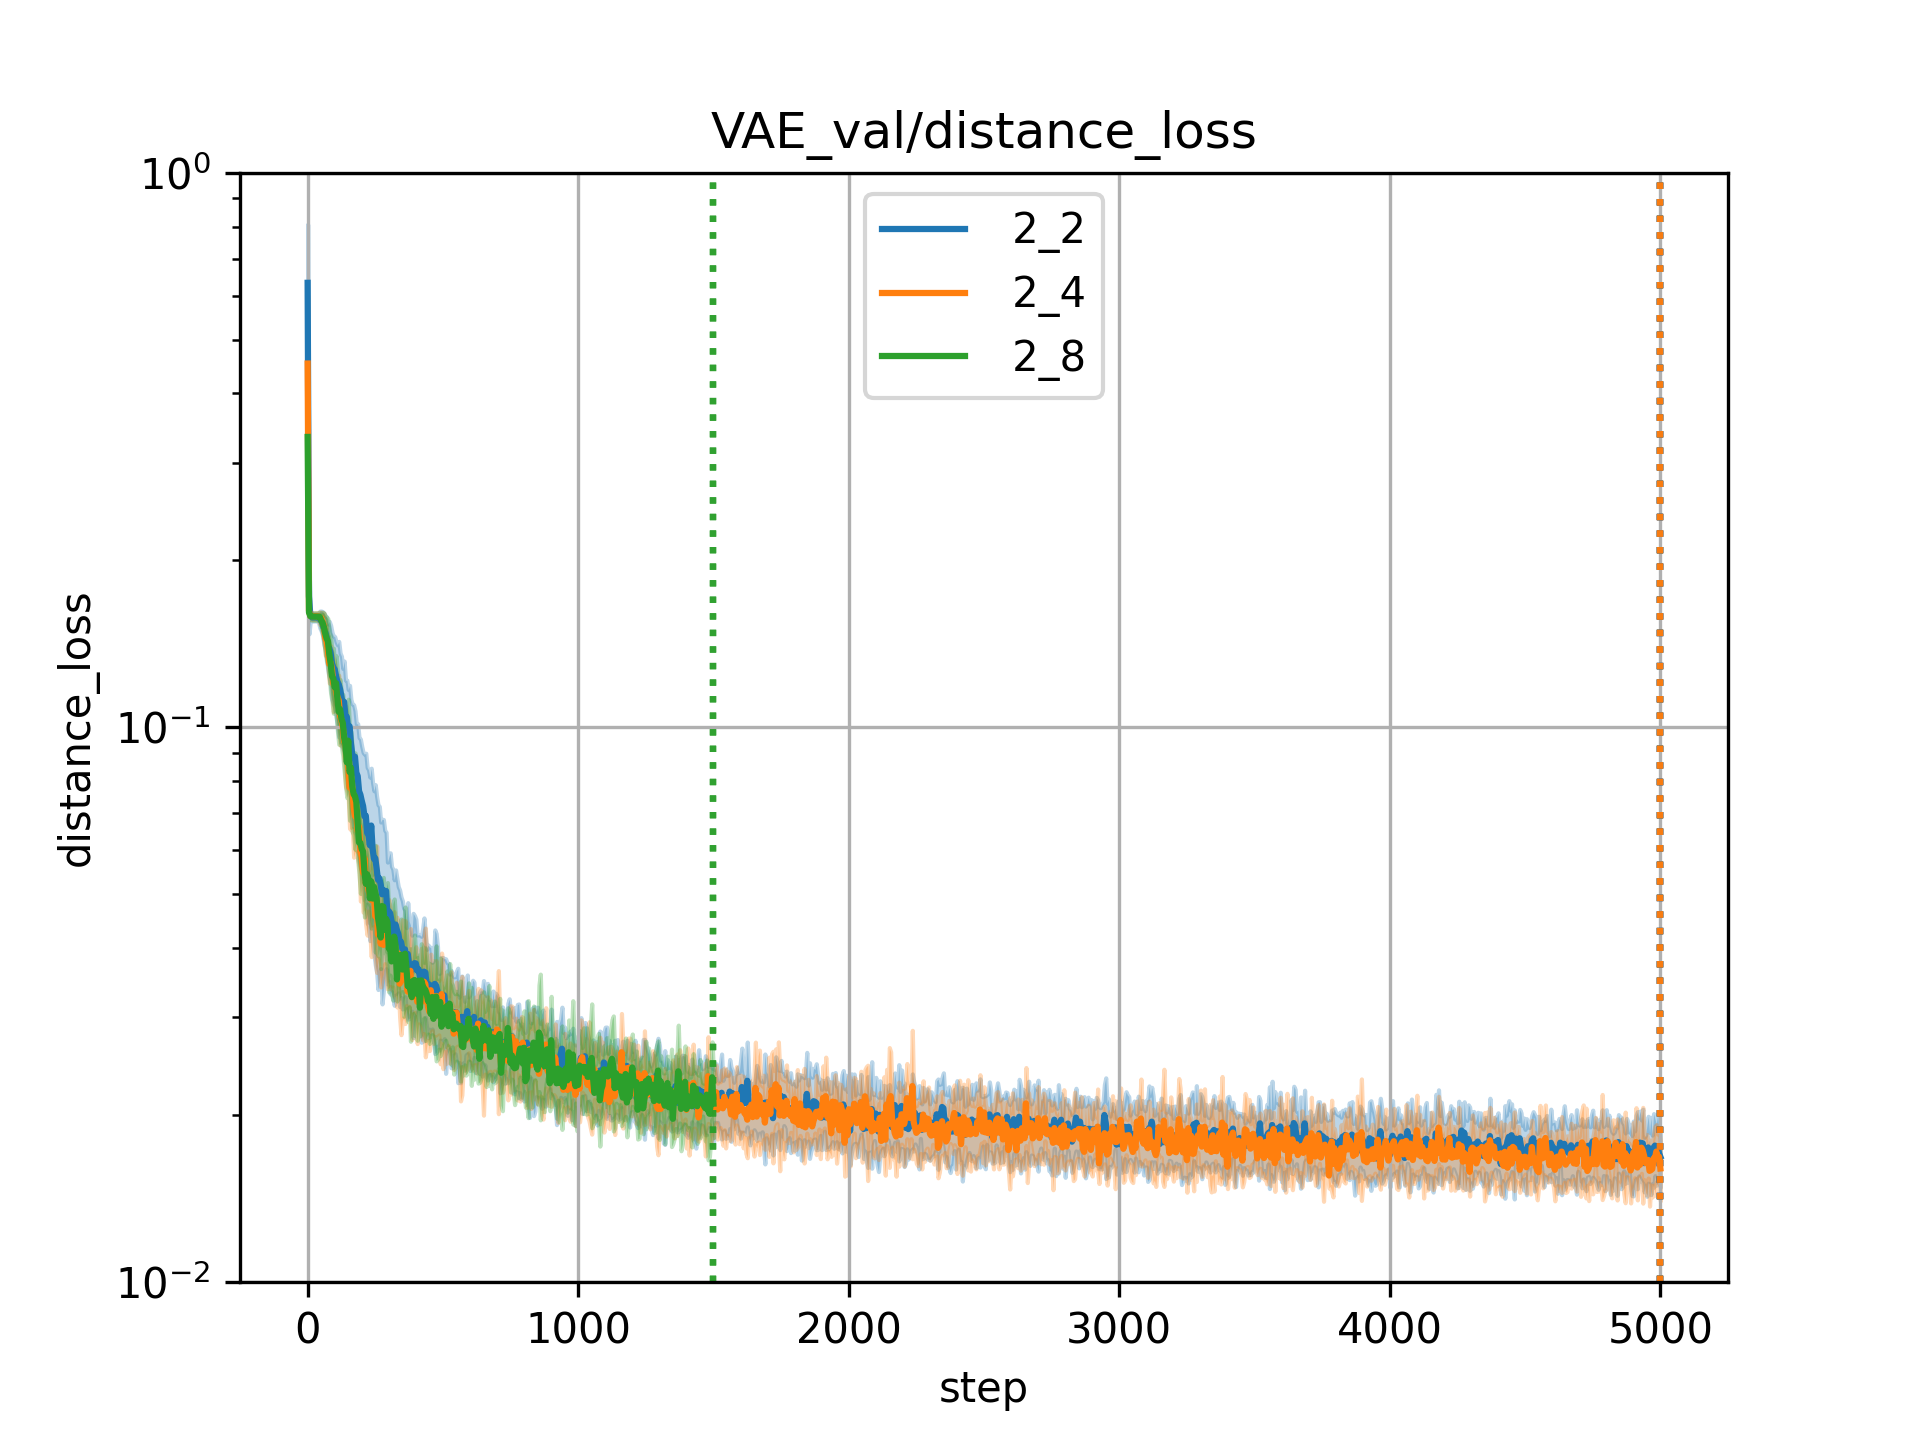
\includegraphics[width=0.23 \linewidth]{figures/experiments/vae_comparison_2_latent_2_4_8_reconstruction_loss.png}
            \label{fig:VAE_latent_comparison_reconstruction_loss/2}
            }
        \hfill
        \subfloat[$N = 5$]{
        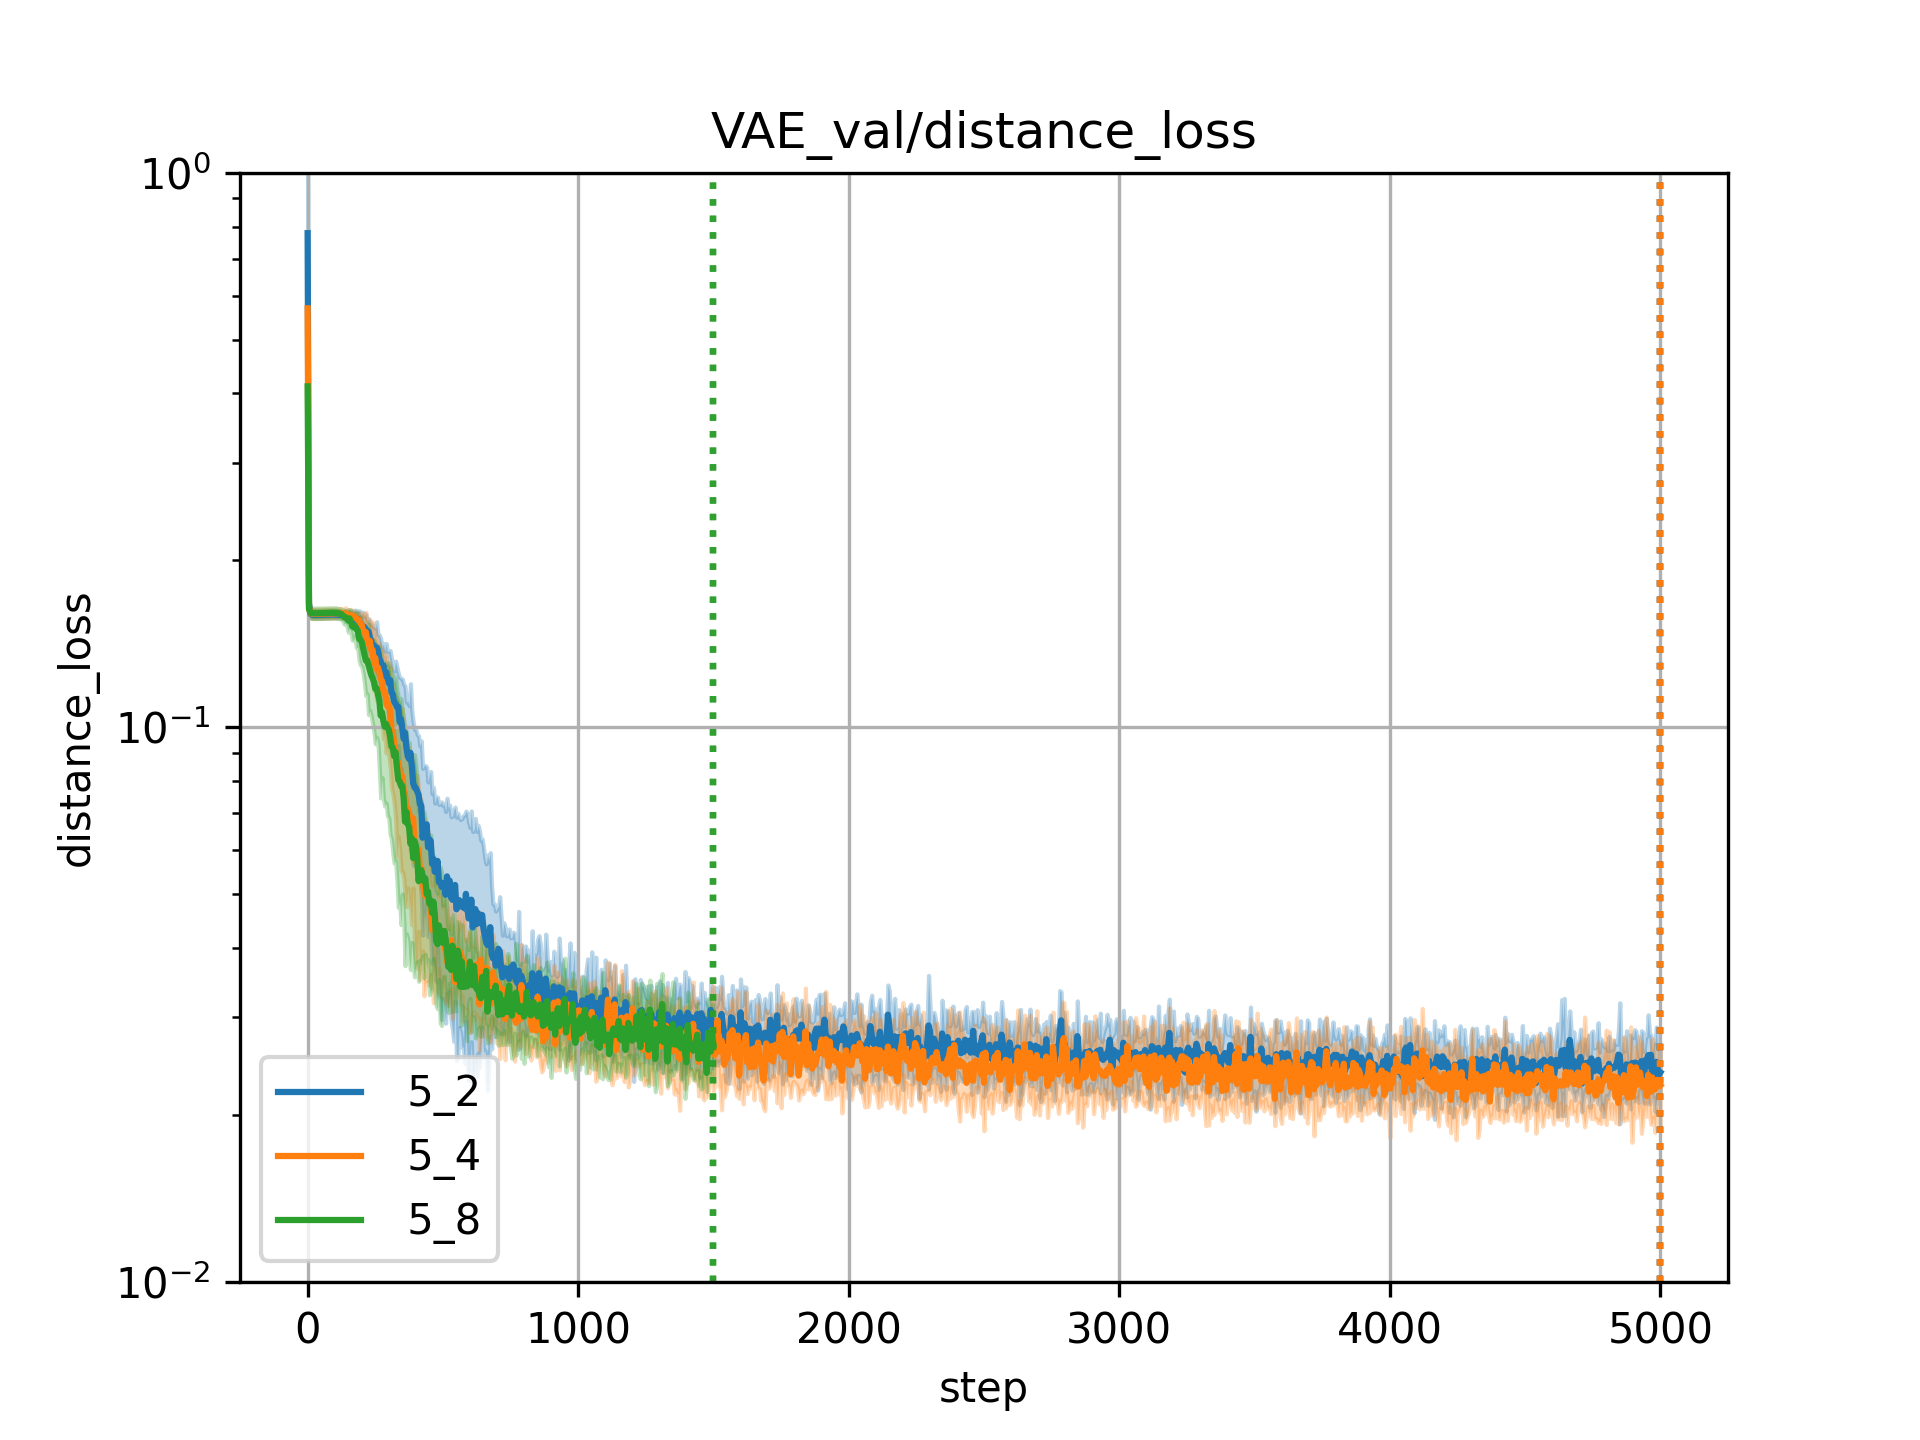
\includegraphics[width=0.23 \linewidth]{figures/experiments/vae_comparison_5_latent_2_4_8_reconstruction_loss.png}
            \label{fig:VAE_latent_comparison_reconstruction_loss/5}
            }
        \hfill
        \subfloat[$N = 10$]{
            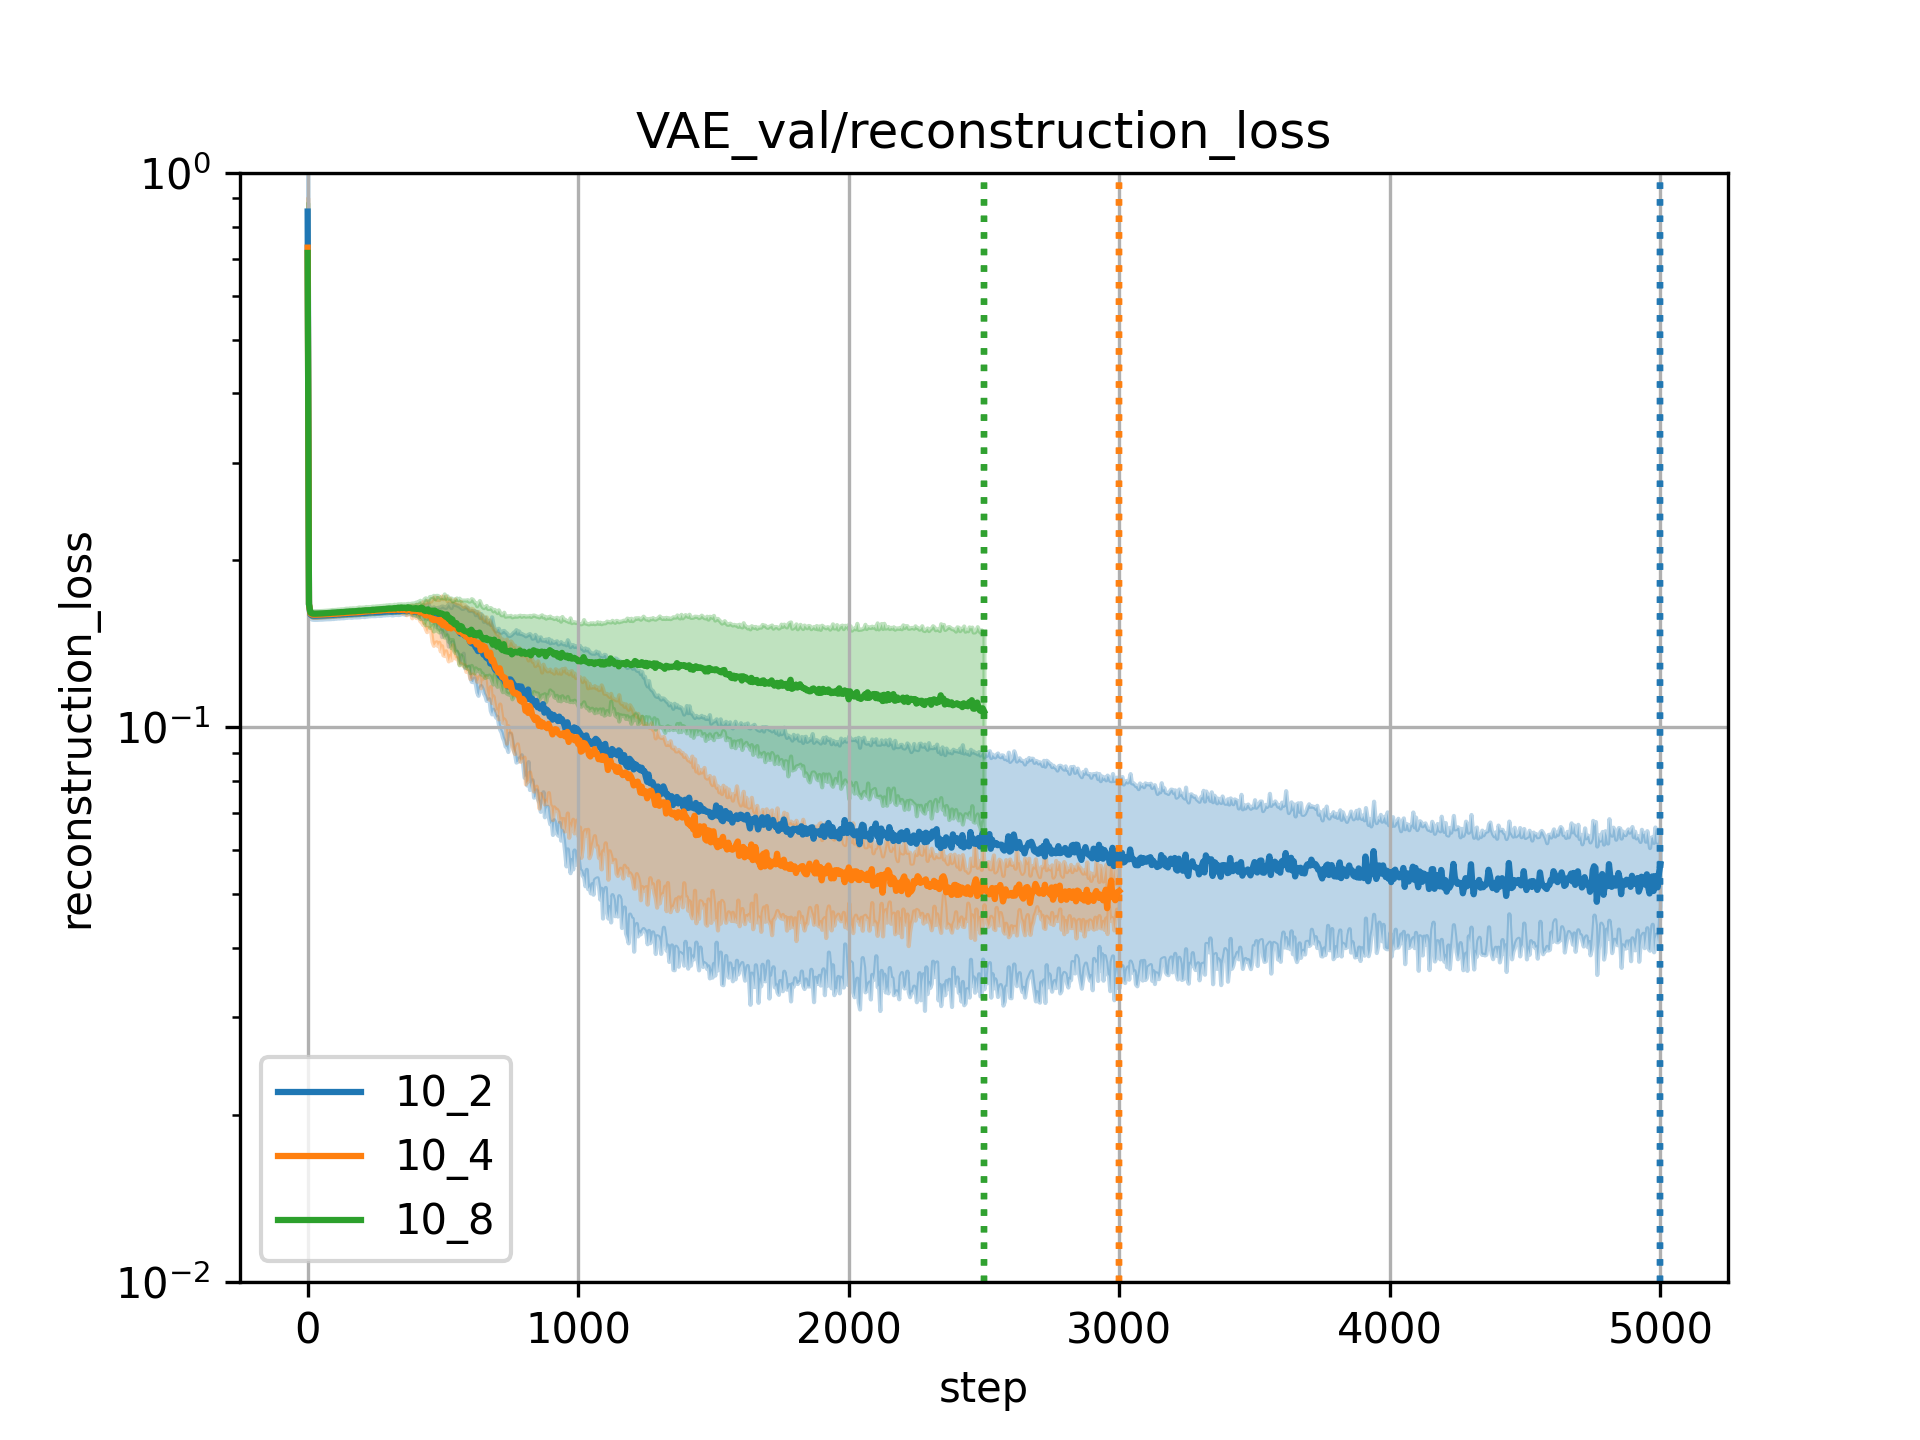
\includegraphics[width=0.23 \linewidth]{figures/experiments/vae_comparison_10_latent_2_4_8_reconstruction_loss.png}
            \label{fig:VAE_latent_comparison_reconstruction_loss/10}
            }
        \hfill
        \subfloat[$N = 15$]{
        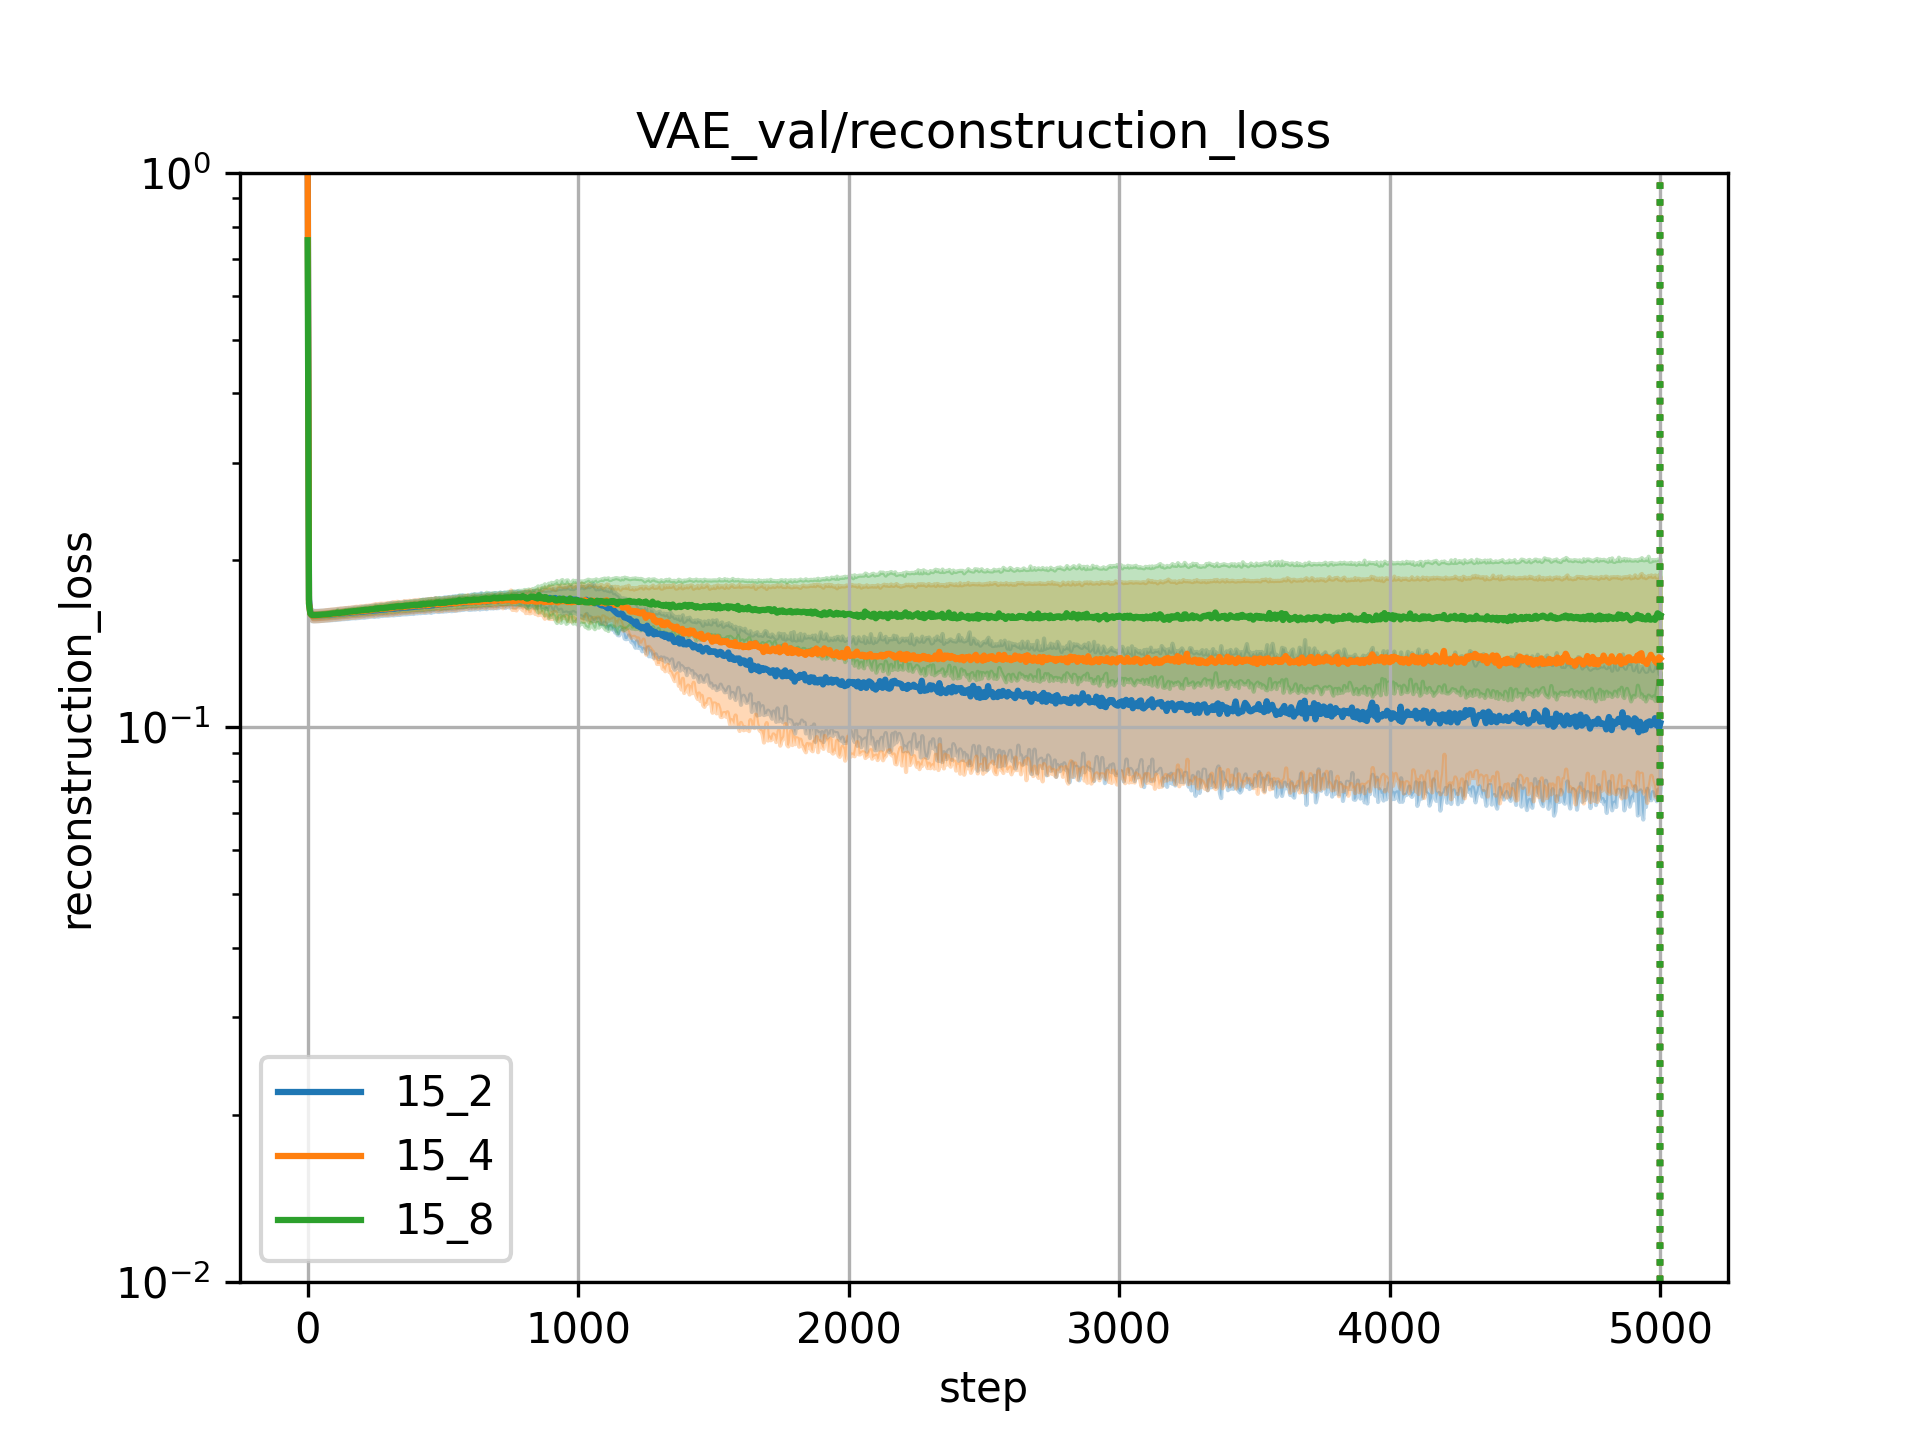
\includegraphics[width=0.23 \linewidth]{figures/experiments/vae_comparison_15_latent_2_4_8_reconstruction_loss.png}
            \label{fig:VAE_latent_comparison_reconstruction_loss/15}
            }
    \end{center}
    \caption[VAE latent dimension comparison on reconstruction loss]{Comparison on the VAE latent dimension based on validation results over different amounts of joints. Each experiment was conducted 10 times with different random seeds. The solid curve is the average over those 10 experiments and the color shaded area resembles the standard deviation. Notice that the y axis in bot plots is in log scale. In the legend each label is structured as \texttt{<$N$>\textunderscore<latent dimension>}}
    \label{fig:VAE_latent_comparison_reconstruction_loss}
\end{figure}

By observing the individual number of joints in each plot of \figref{fig:VAE_latent_comparison_reconstruction_loss} form (a) to (d) we can observe that the latent dimension does make a difference in the final reconstruction loss performances. Starting with two joints there is no significant difference between the latent dimensions of two to eight. Continuing with 5 joints we can observe no significant difference in the finial performance but a slight difference with respect of how fast the models are converging. The experiments on a latent dimension of four and eight are very similar while the standard deviation for a latent dimension equal to two increases around 600 epochs indicating that some experiments have slight troubles to converge. \\
A significant difference in final performance can be observed with $N = 10$. Here the best performance is returned by experiments with a latent dimension of four closely followed by two. Comparing two and four in \figref{fig:VAE_latent_comparison_reconstruction_loss/10} shows that four is much more stable and faster in learning the problem as two. Last ranked are the experiments for a latent dimension of eight. Those experiments are by far not on the same level as with a latent dimension of two and four. A deeper look into the inference shows that the model fails to come up with an action to reach the given target position.\\
In \figref{fig:VAE_latent_comparison_reconstruction_loss/15} a performance difference is noticeable with a latent dimension of two as best and eight as worst. But since the best performance of the experiments with a latent dimension of two is on the same level as eight in \figref{fig:VAE_latent_comparison_reconstruction_loss/10} we can conclude that the the VAE fails at $N = 15$ with the present hyperparameter as in \tabref{tab:VAE_Hyperparameters}.

\subsubsection{Distance and Imitation Loss}

In this section we are going to present the results of training the VAE with the imitation loss to pre-calculated solutions from \algoref{alg:CCD}. The important change in the config file is setting \texttt{dataset target mode = ACTION} to tell the dataset to also calculate action from ccd.  

Because of time limitation we applied this loss function only on a setting with a latent dimension of four since this was the best latent dimension fitted only with the distance loss. 

All in all the distance loss functions in \figref{fig:VAE_imitation/distance_loss} yield almost the same examples as the distance loss functions in \figref{fig:VAE_latent/reconstruction_4}.\\
Additional to the distance loss we have got also an imitation loss between the computed action from  CCD and the action yielded from form the neural Network in \figref{fig:VAE_imitation/imitation_loss}. Here it is interesting to note that the imitation loss is increasing alongside $N$ but not in the same scale. Where the differences between the imitation losses are becoming smaller for bigger $N$. Another thing that is particular interesting is the convergence behavior of each curve. They all hav a huge drop in the beginning but stay on their level for the rest of the training as if the have reached their optimal value. \\
Finally looking at the KL-divergence we do can note an almost indistinguishable plot form \figref{fig:VAE_latent/kl_4}.

\begin{figure}
    \begin{center}
        \subfloat[Distance loss]{
        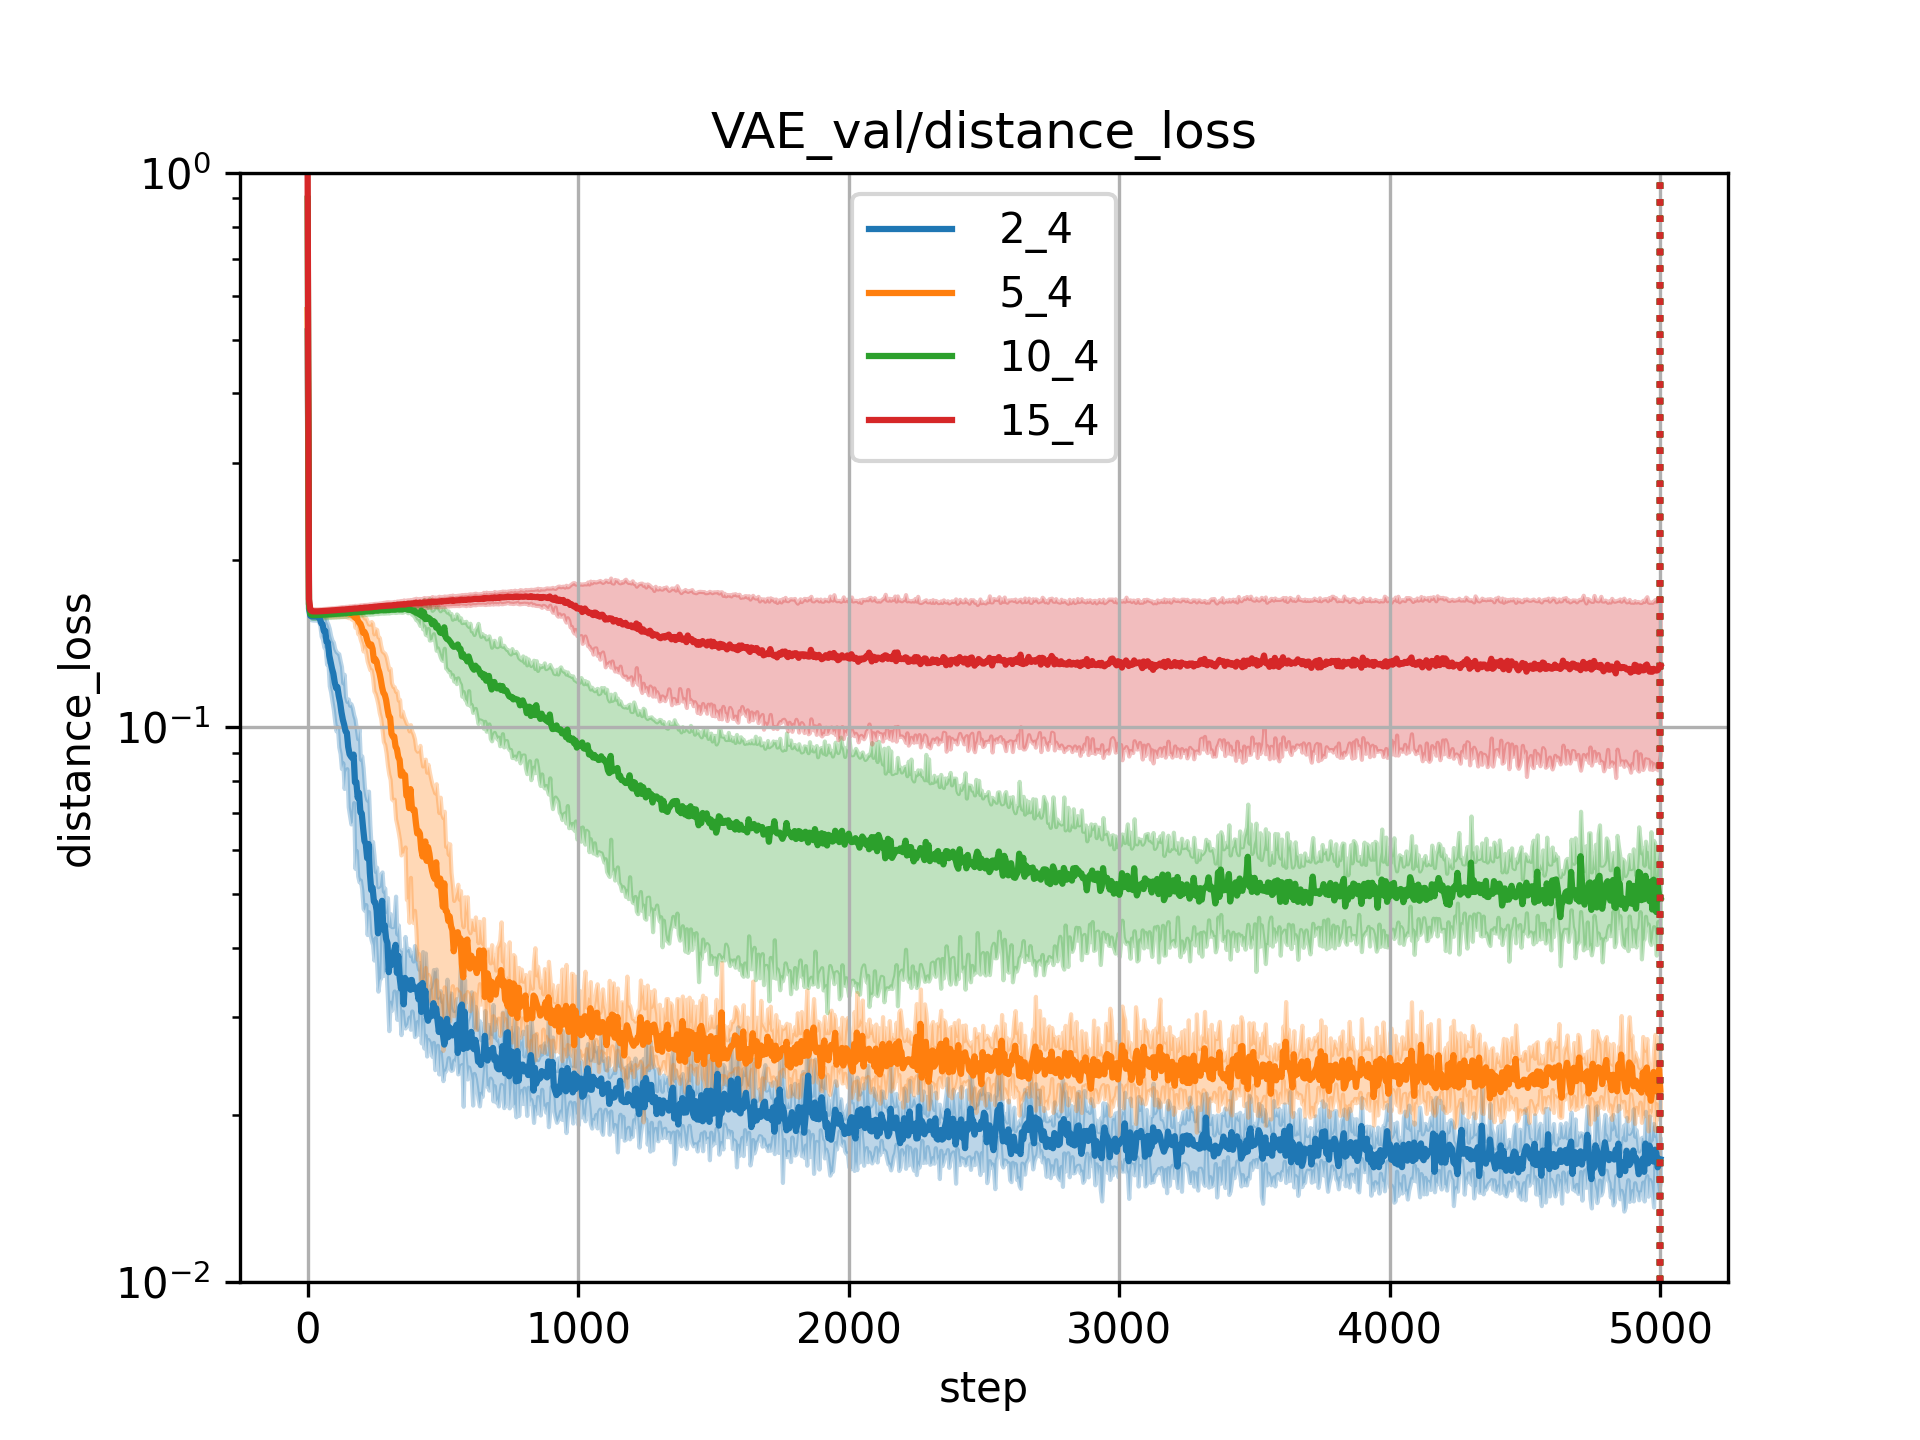
\includegraphics[width=0.31 \linewidth]{figures/experiments/vae_comparison_imitation_[2, 5, 10, 15]_latent_4 4 4 4_distance_loss.png}
            \label{fig:VAE_imitation/distance_loss}
            }
        \hfill
        \subfloat[Imitation loss]{
        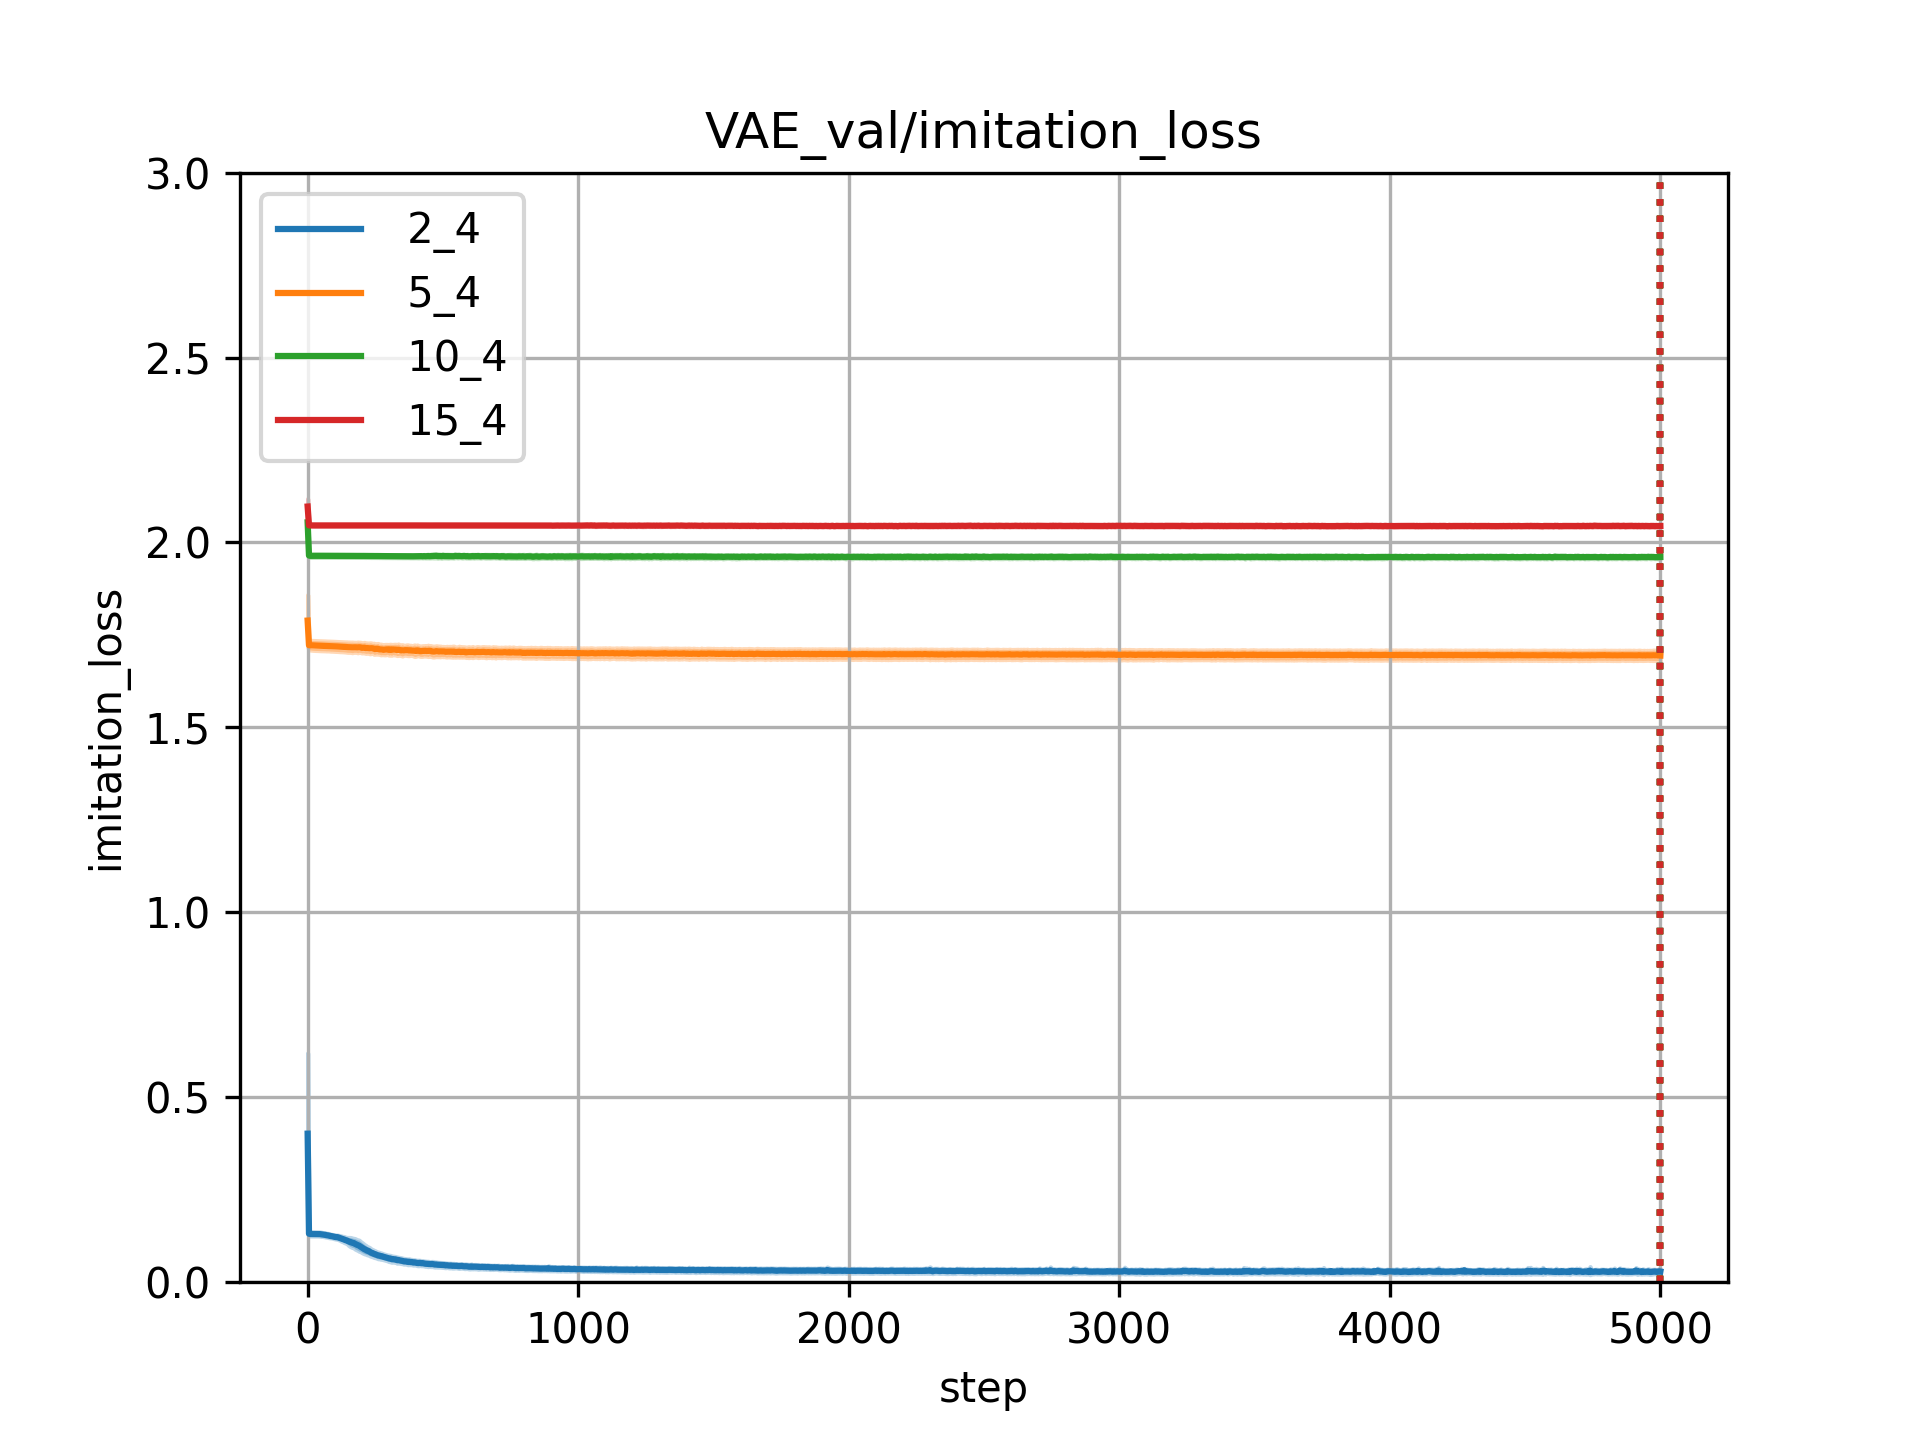
\includegraphics[width=0.31 \linewidth]{figures/experiments/vae_comparison_imitation_[2, 5, 10, 15]_latent_4 4 4 4_imitation_loss.png}
            \label{fig:VAE_imitation/imitation_loss}
            }
        \hfill
        \subfloat[KL diveregence from standard normal distribution]{
        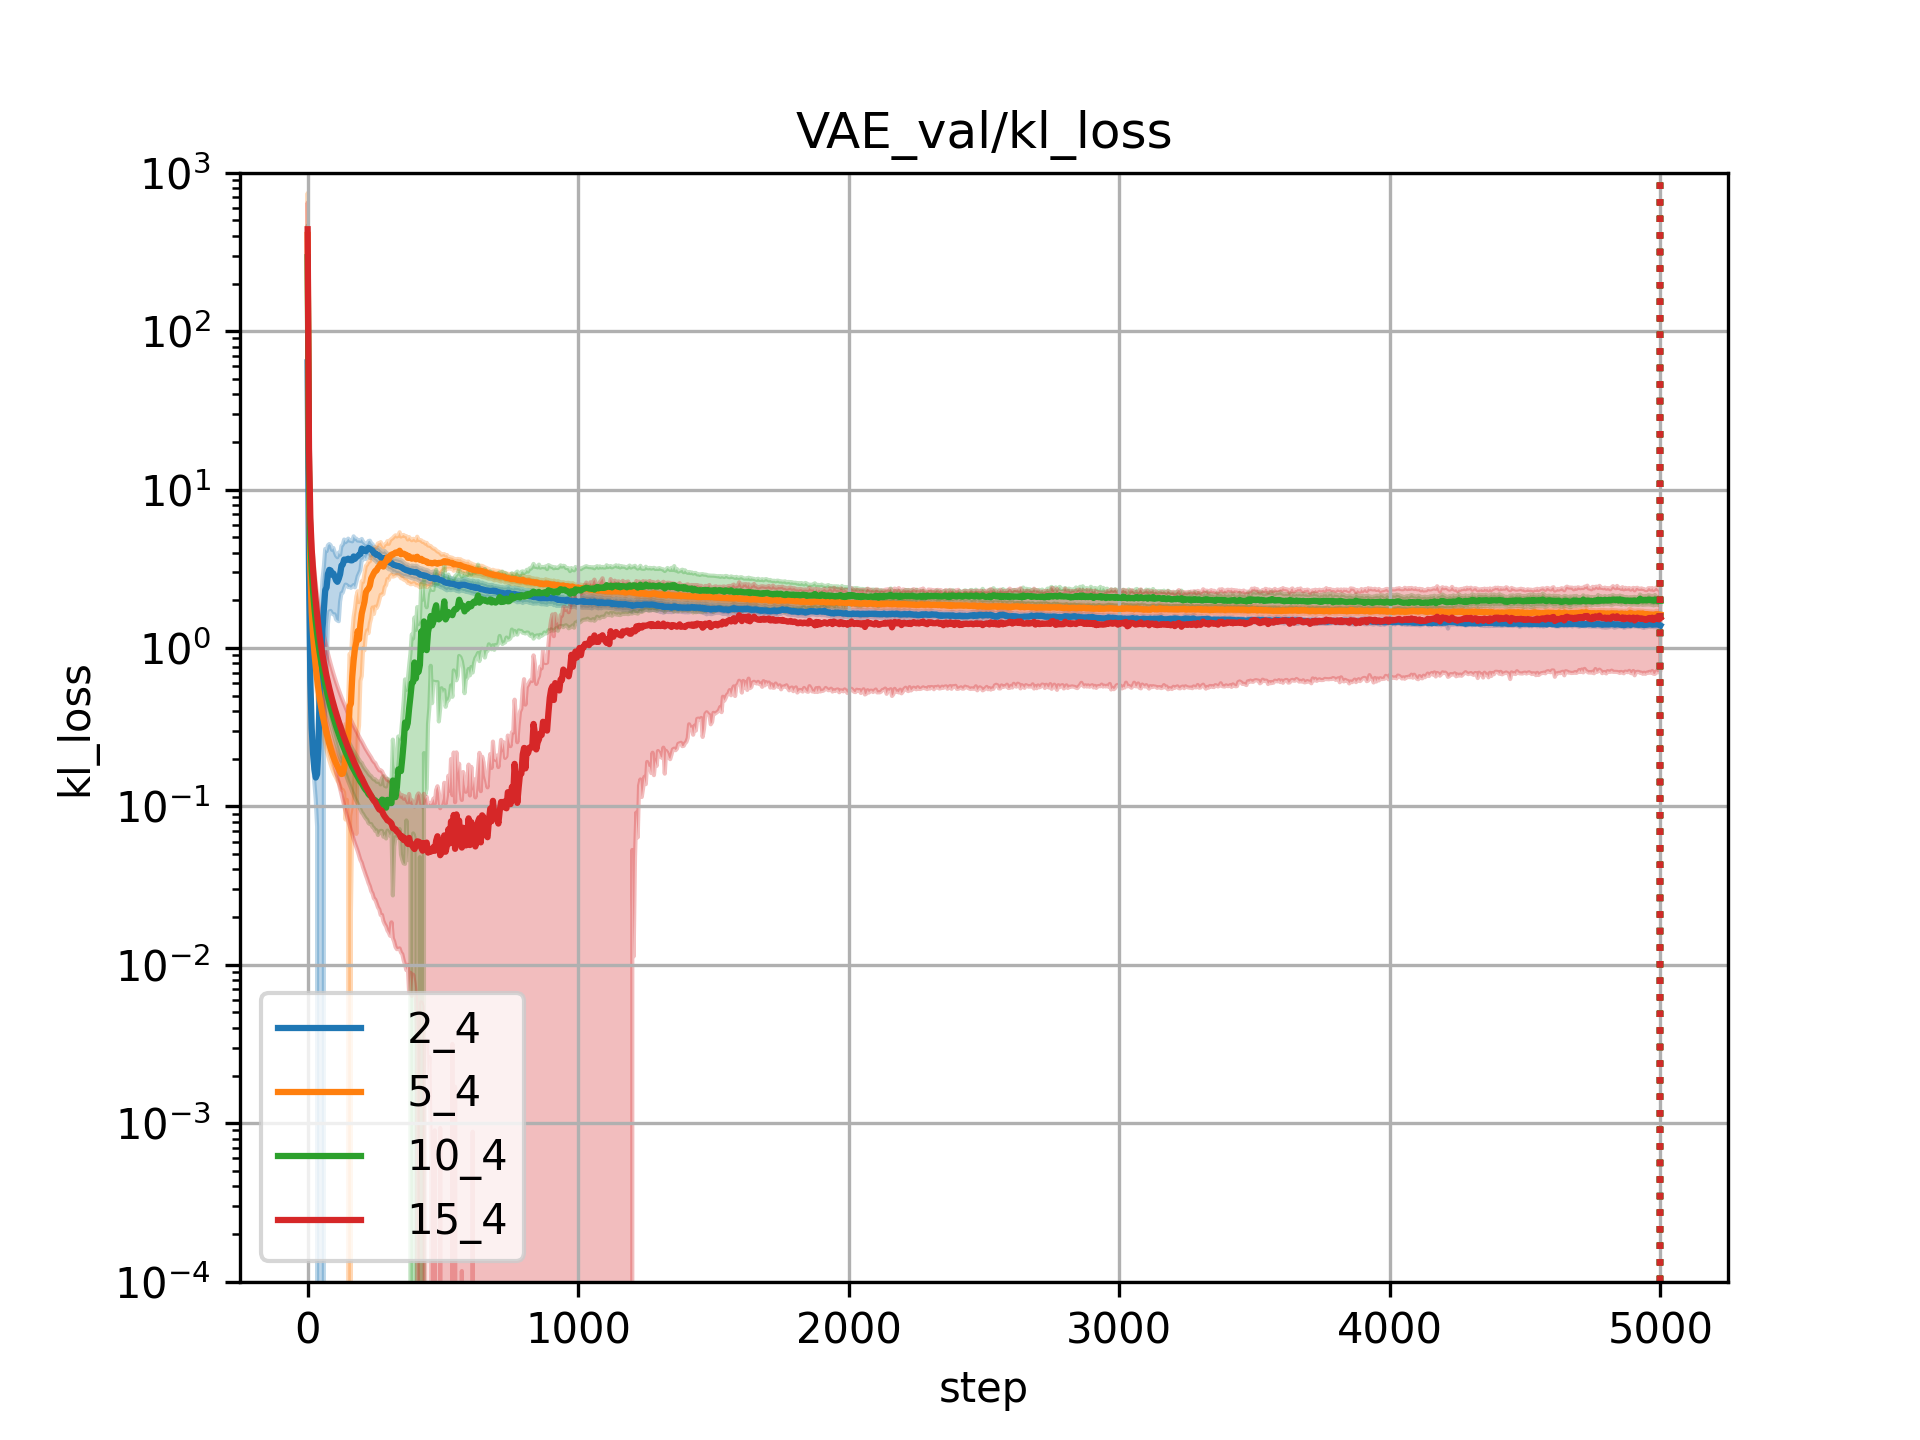
\includegraphics[width=0.31 \linewidth]{figures/experiments/vae_comparison_imitation_[2, 5, 10, 15]_latent_4 4 4 4_kl_loss.png}
            \label{fig:VAE_imitation/kl_loss}
            }
    \end{center}
    \caption[VAE validation results with imitation loss]{Results on the validation dataset while training a VAE with a latent dimension of 4 but incorporating an imitation loss weighted with 0.01. Results are collected from ten different runs and with a solid mean curve and a shaded standard deviation area. $N \in [2, 5, 10, 15]$} 
    \label{fig:VAE_imitation}
\end{figure}

\subsection{Supervised}

For the supervised actions we only relied on state information as the input to predict an action to reach from the current state the given target position.  Since this approach is very similar to the Variational Autoencoder setting we are also able to apply the afore mentioned Inverse Kinematics Loss with distance and imitation loss as in \eqref{eqn:IK-Loss}.

The results of the supervised experiments are divided into two parts. The first is only applying the distance loss while the second one is incorporating also an imitation loss with respect ot pre computed actions from the CCD solver.

\subsubsection{Distance Loss}

The distance loss results over different amount of joints in \figref{fig:supervised_distance} are very similar compared to \figref{fig:VAE_latent} (a) to (c). Parallel to \figref{fig:VAE_latent} we can also observe an overall increase in loss while increasing $N$ and finishing at different convergence levels. Different to the experiments on the VAE is the standard deviation between the experiments. The supervised experiments show a significant smaller standard deviation across the whole training period compared to the VAE experiments.

\begin{figure}
    \begin{center}
        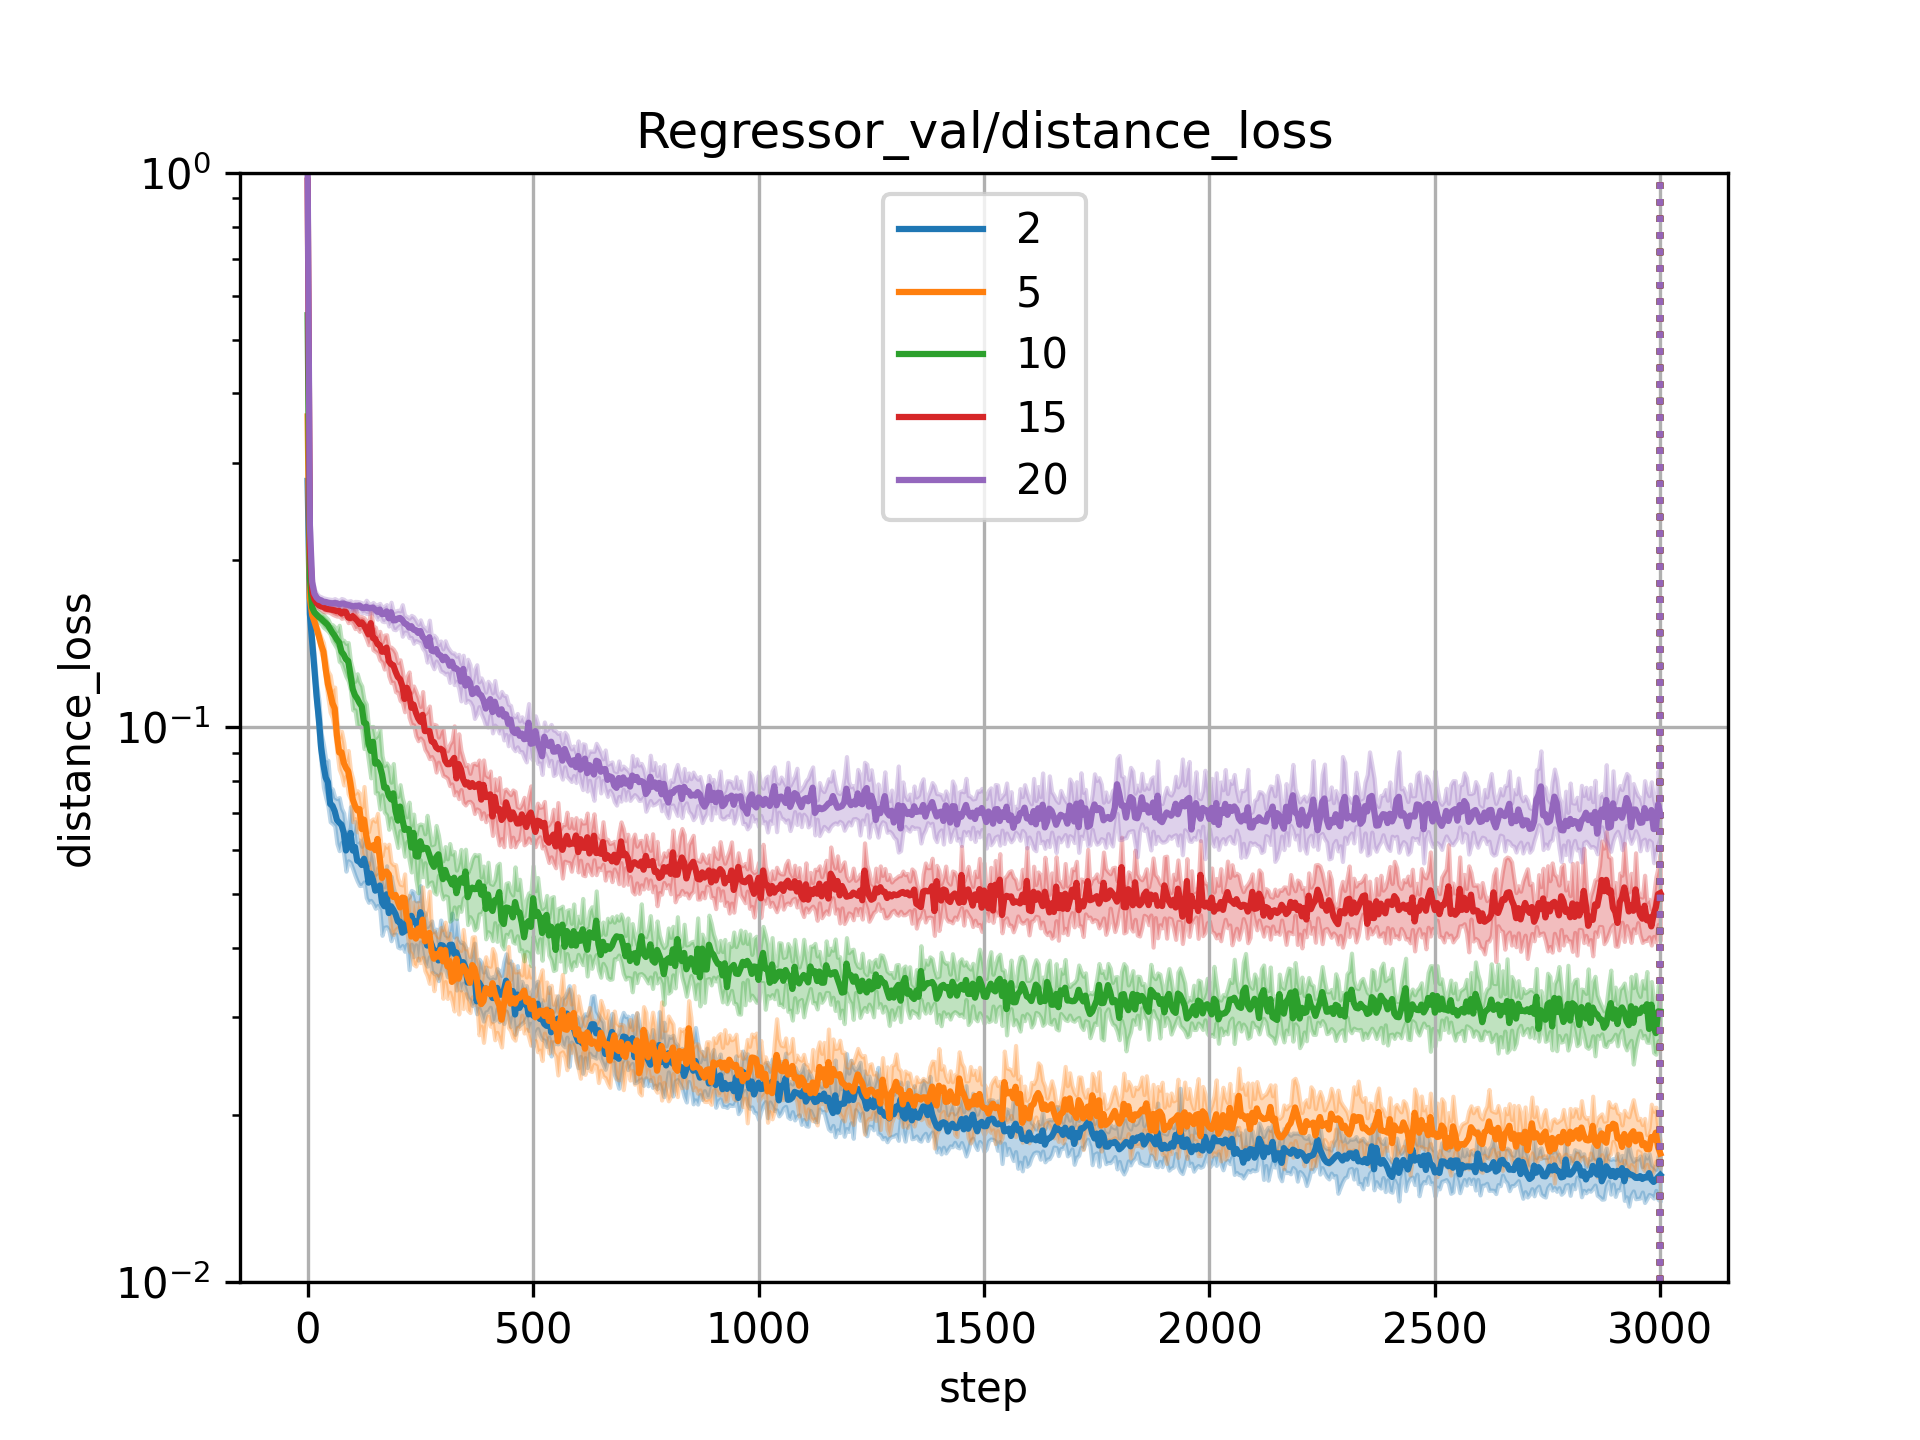
\includegraphics[width=0.46 \linewidth]{figures/experiments/supervised_2_distance_loss.png}
    \end{center}
    \caption[Supervised Distance Loss]{Distance loss for supervised experiments over different $N \in [2, 5, 10, 15, 20]$. For each $N$ we conducted 10 experiments. }
    \label{fig:supervised_distance}
\end{figure}

\subsubsection{Distance and Imitation Loss}

For this series of experiments we also want to emphasis solutions close to solutions computed by the CCD by setting the dataset mode to \texttt{ACTION} and setting the imitation loss weight to 0.01. 

Unlike as in the previous section the distance loss differs a lot from \figref{fig:supervised_distance}. We do not see a steady increase in loss over different numbers of joints instead we do see vastly different levels of final distance loss performances starting with two joints at around 1.1 and ending with 15 joints at XXX.\\
A bit more interesting are the results on the imitation loss. Similar to \figref{fig:VAE_imitation/imitation_loss} all curves have a drop in the first couple of epochs but are constant for the rest of the training. Comparing those curves with respect to the number of joints we observed that all mean curves have vastly different levels of convergence which seems not to be linear correlated with $N$.


\begin{figure}
    \begin{center}
        \subfloat[Distance Loss]{
            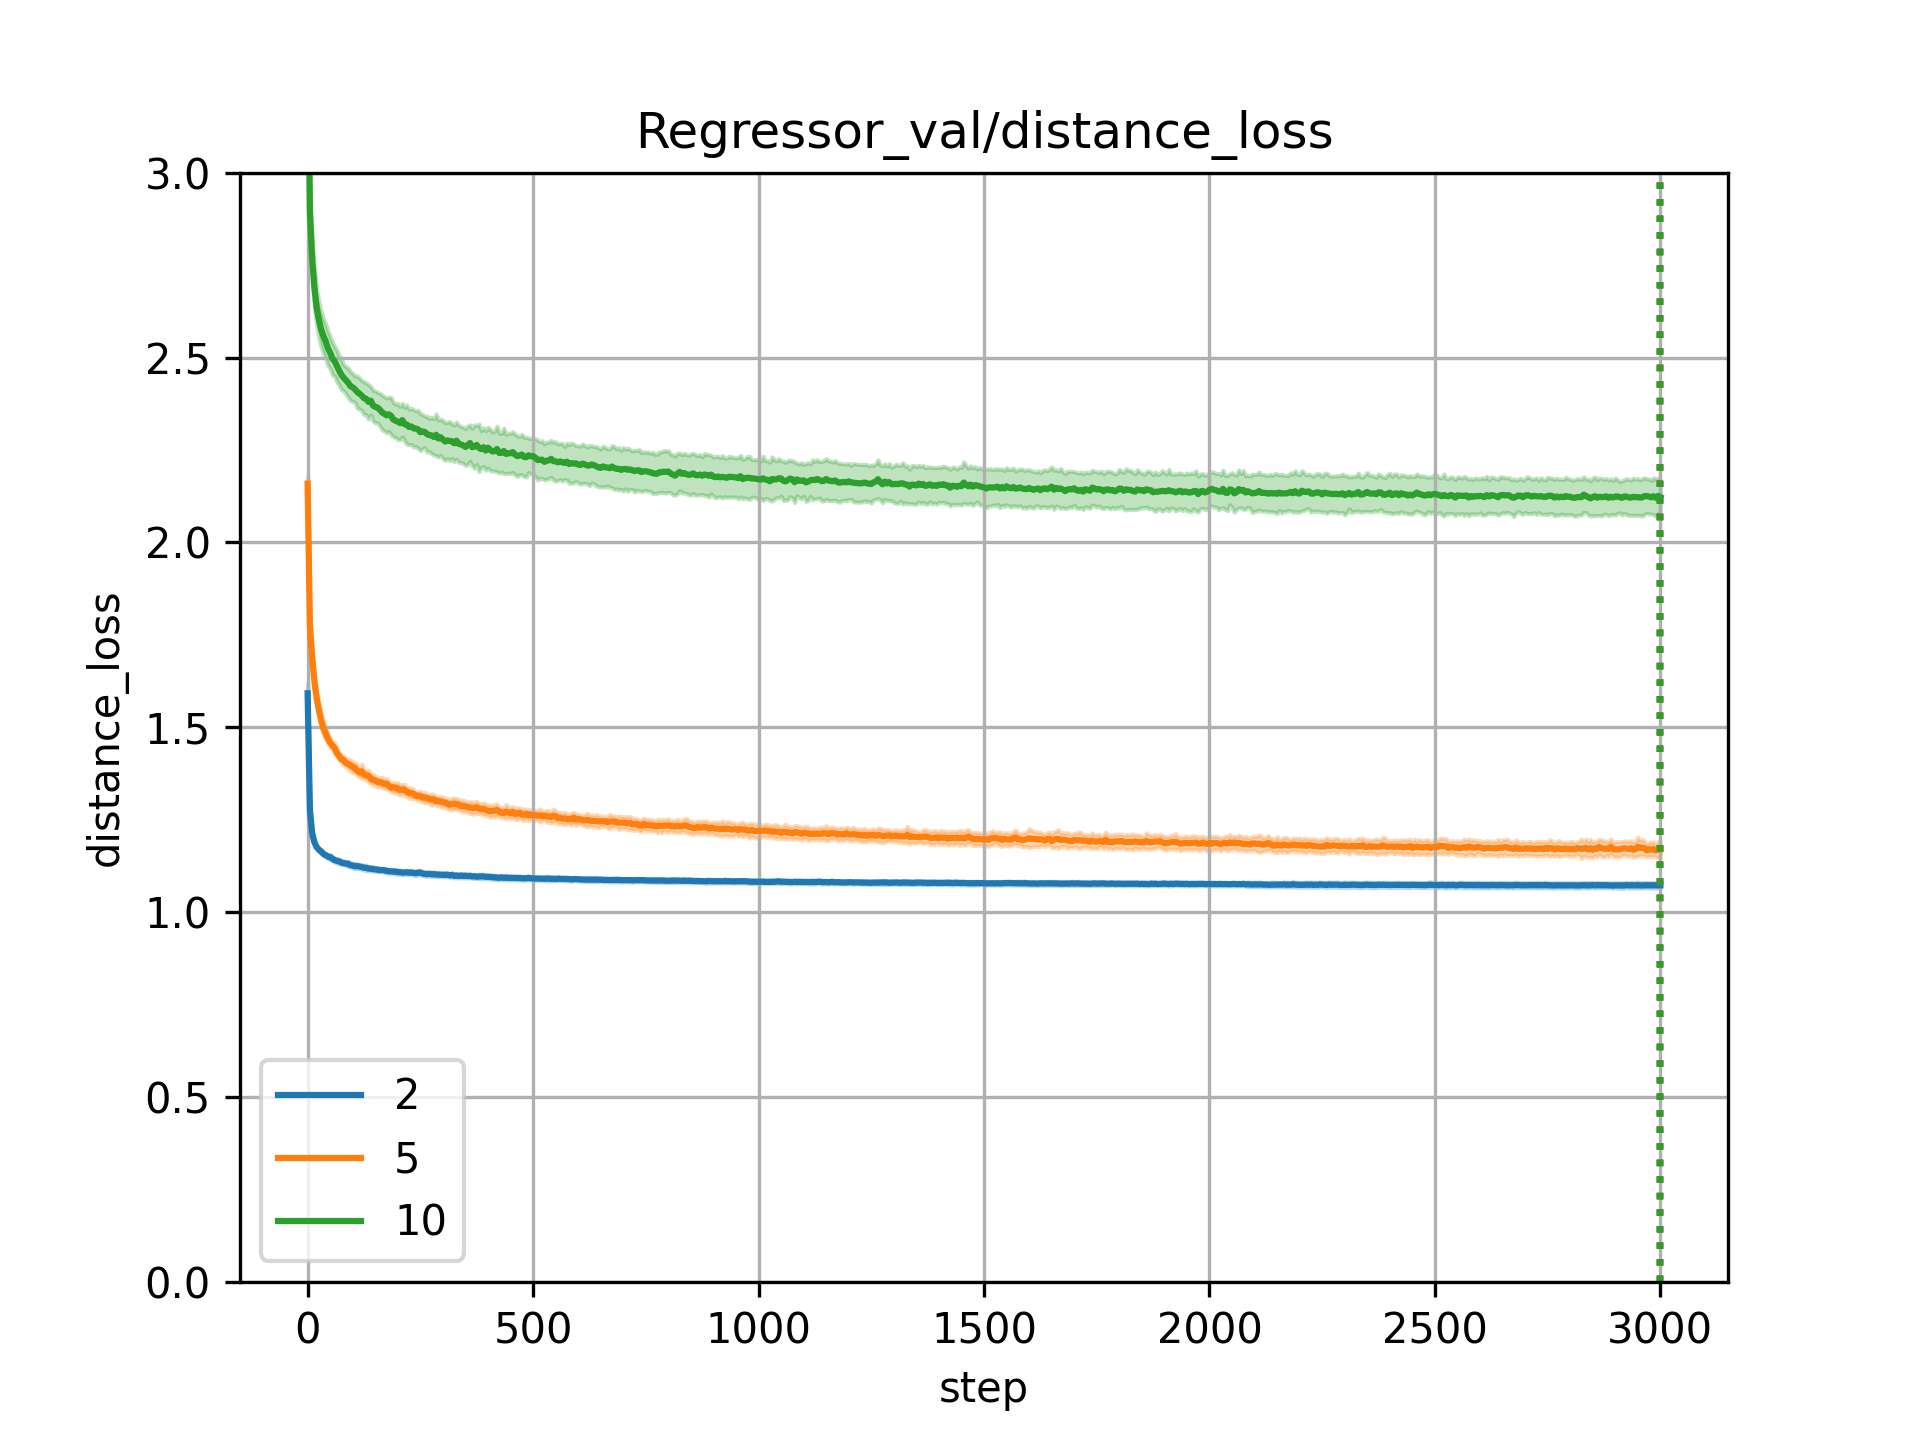
\includegraphics[width=0.46 \linewidth]{figures/experiments/supervised_imitation_2_latent_4 4 4 4_distance_loss.png}
            \label{fig:supervised_imitation/distance_loss}
            }
        \hfill
        \subfloat[Imitation Loss]{
        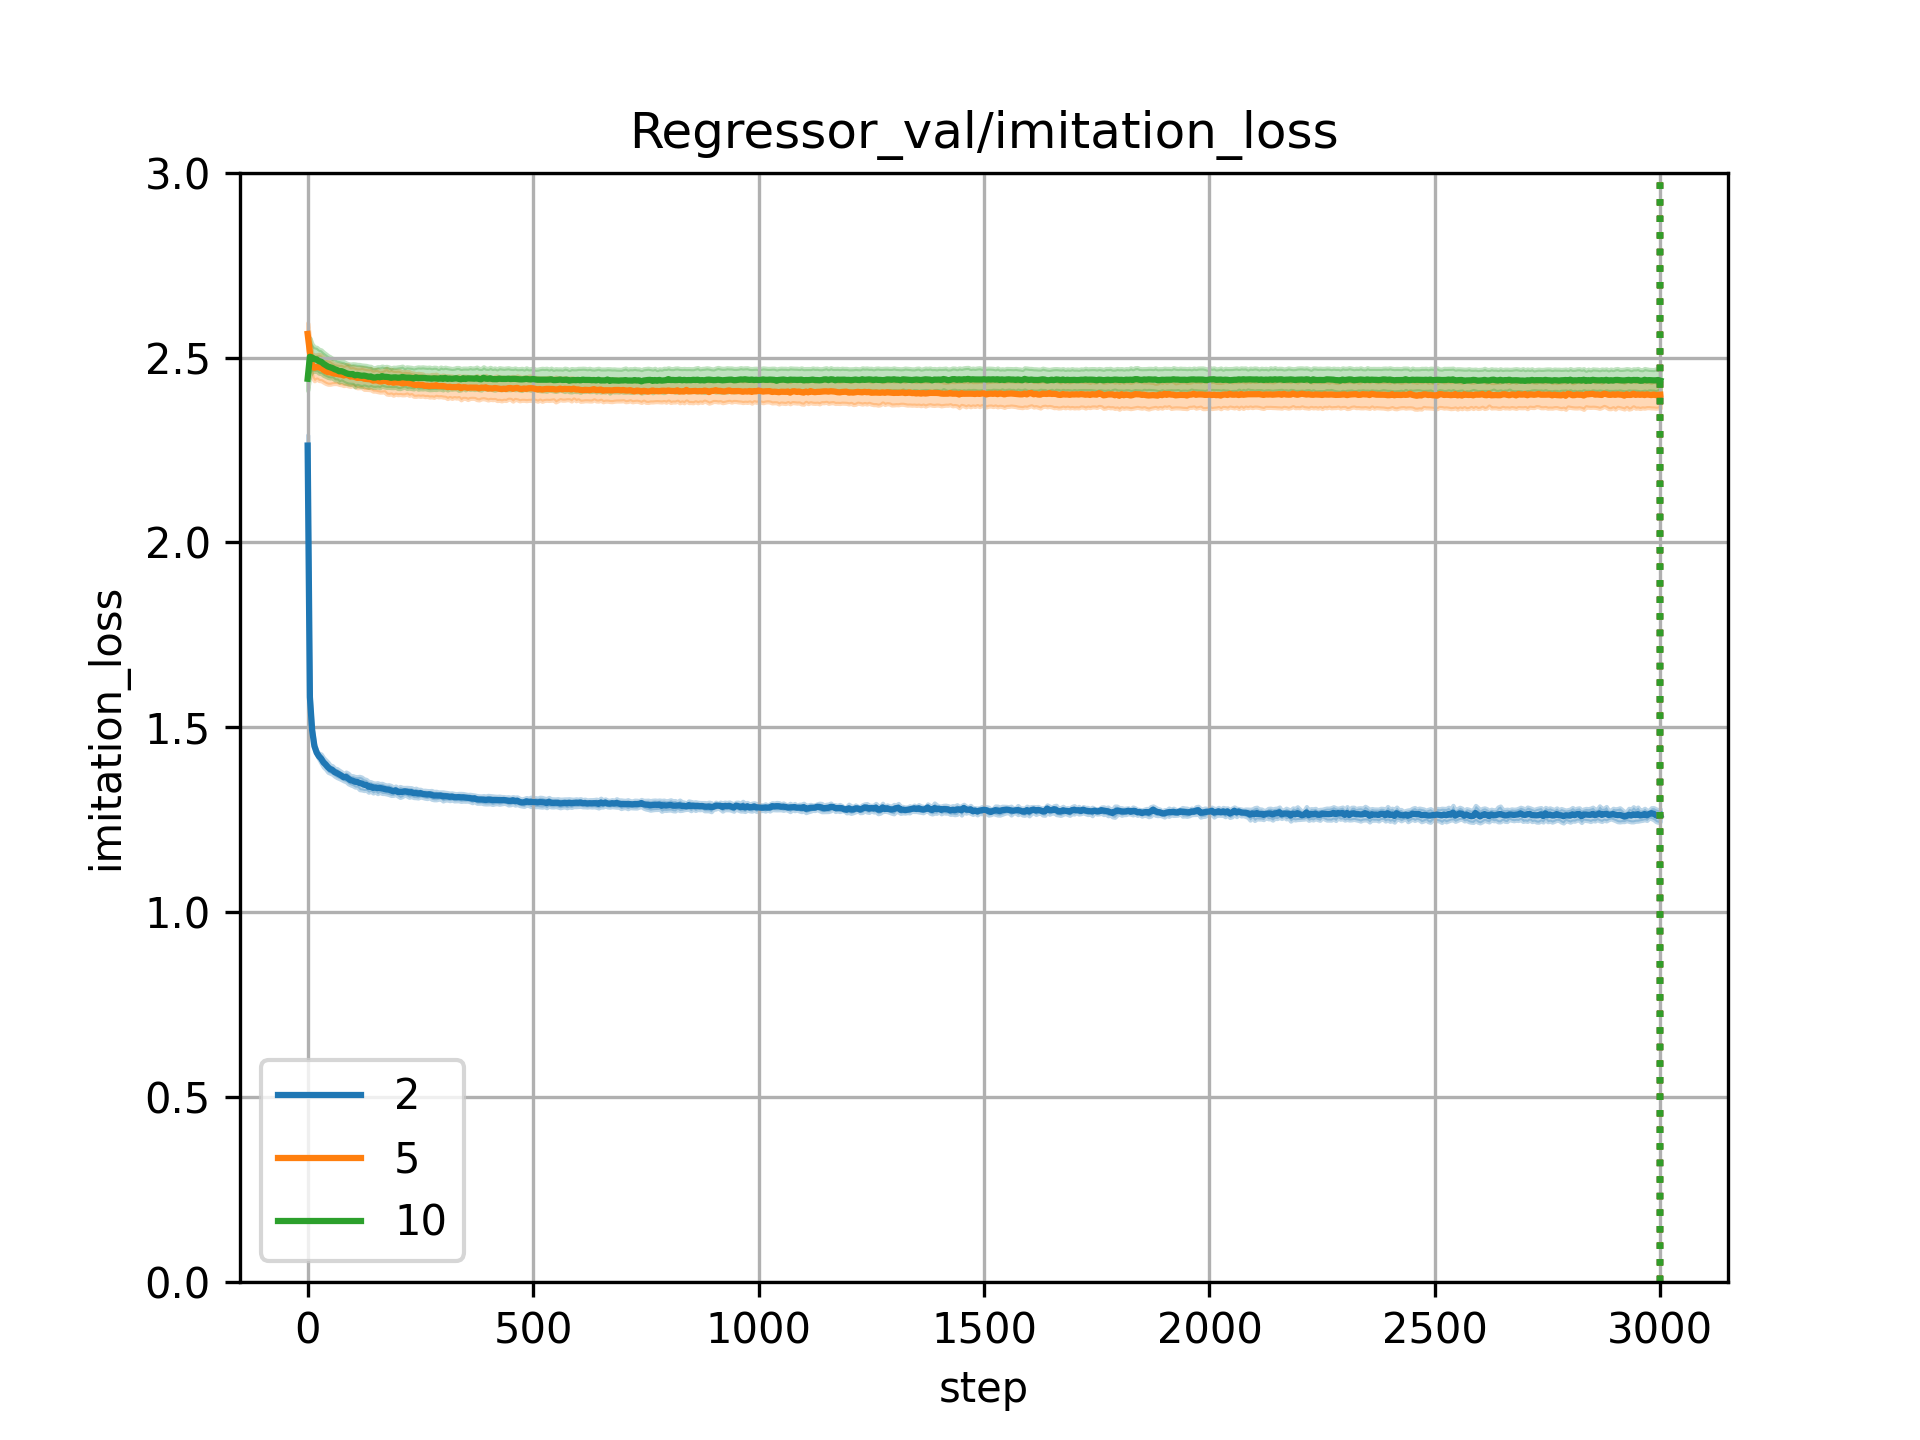
\includegraphics[width=0.46 \linewidth]{figures/experiments/supervised_imitation_2_latent_4 4 4 4_imitation_loss.png}
            \label{fig:supervised_imitation/imitation_loss}
            }
    \end{center}
    \caption[Supervised Distance and Imitation Loss]{Validation results for supervised experiments on distance and imitation loss. }
    \label{fig:supervised_imitation}
\end{figure}

\section{Reinforcement Learning}

In this section we will present results on the reinforcement learning experiments on the 2D inverse kinematics environment. \\
First we will set a benchmark with the plane Soft Actor-Critic. Further we will combine Soft Actor-Critic with pre-trained latent models and have a look into their performance statistics but also comparing it to the plane Soft Actor-Critic results. 

\subsection{Baseline Soft Actor-Critic}

First we would like to have a look how a the plain SAC algorithm, where the actor network directly calculates actions for the environment, performs on the inverse kinematics environment as described in \secref{sec:RL-Environment}. Further we will describe this kind of experiments as SAC baseline experiments. All Hyperparameters used for the SAC baseline experiments can be found in \chapref{chap:appendix}.
\begin{figure}
    \begin{center}
        \subfloat[Mean reward per step over the last 20 episodes.]{
            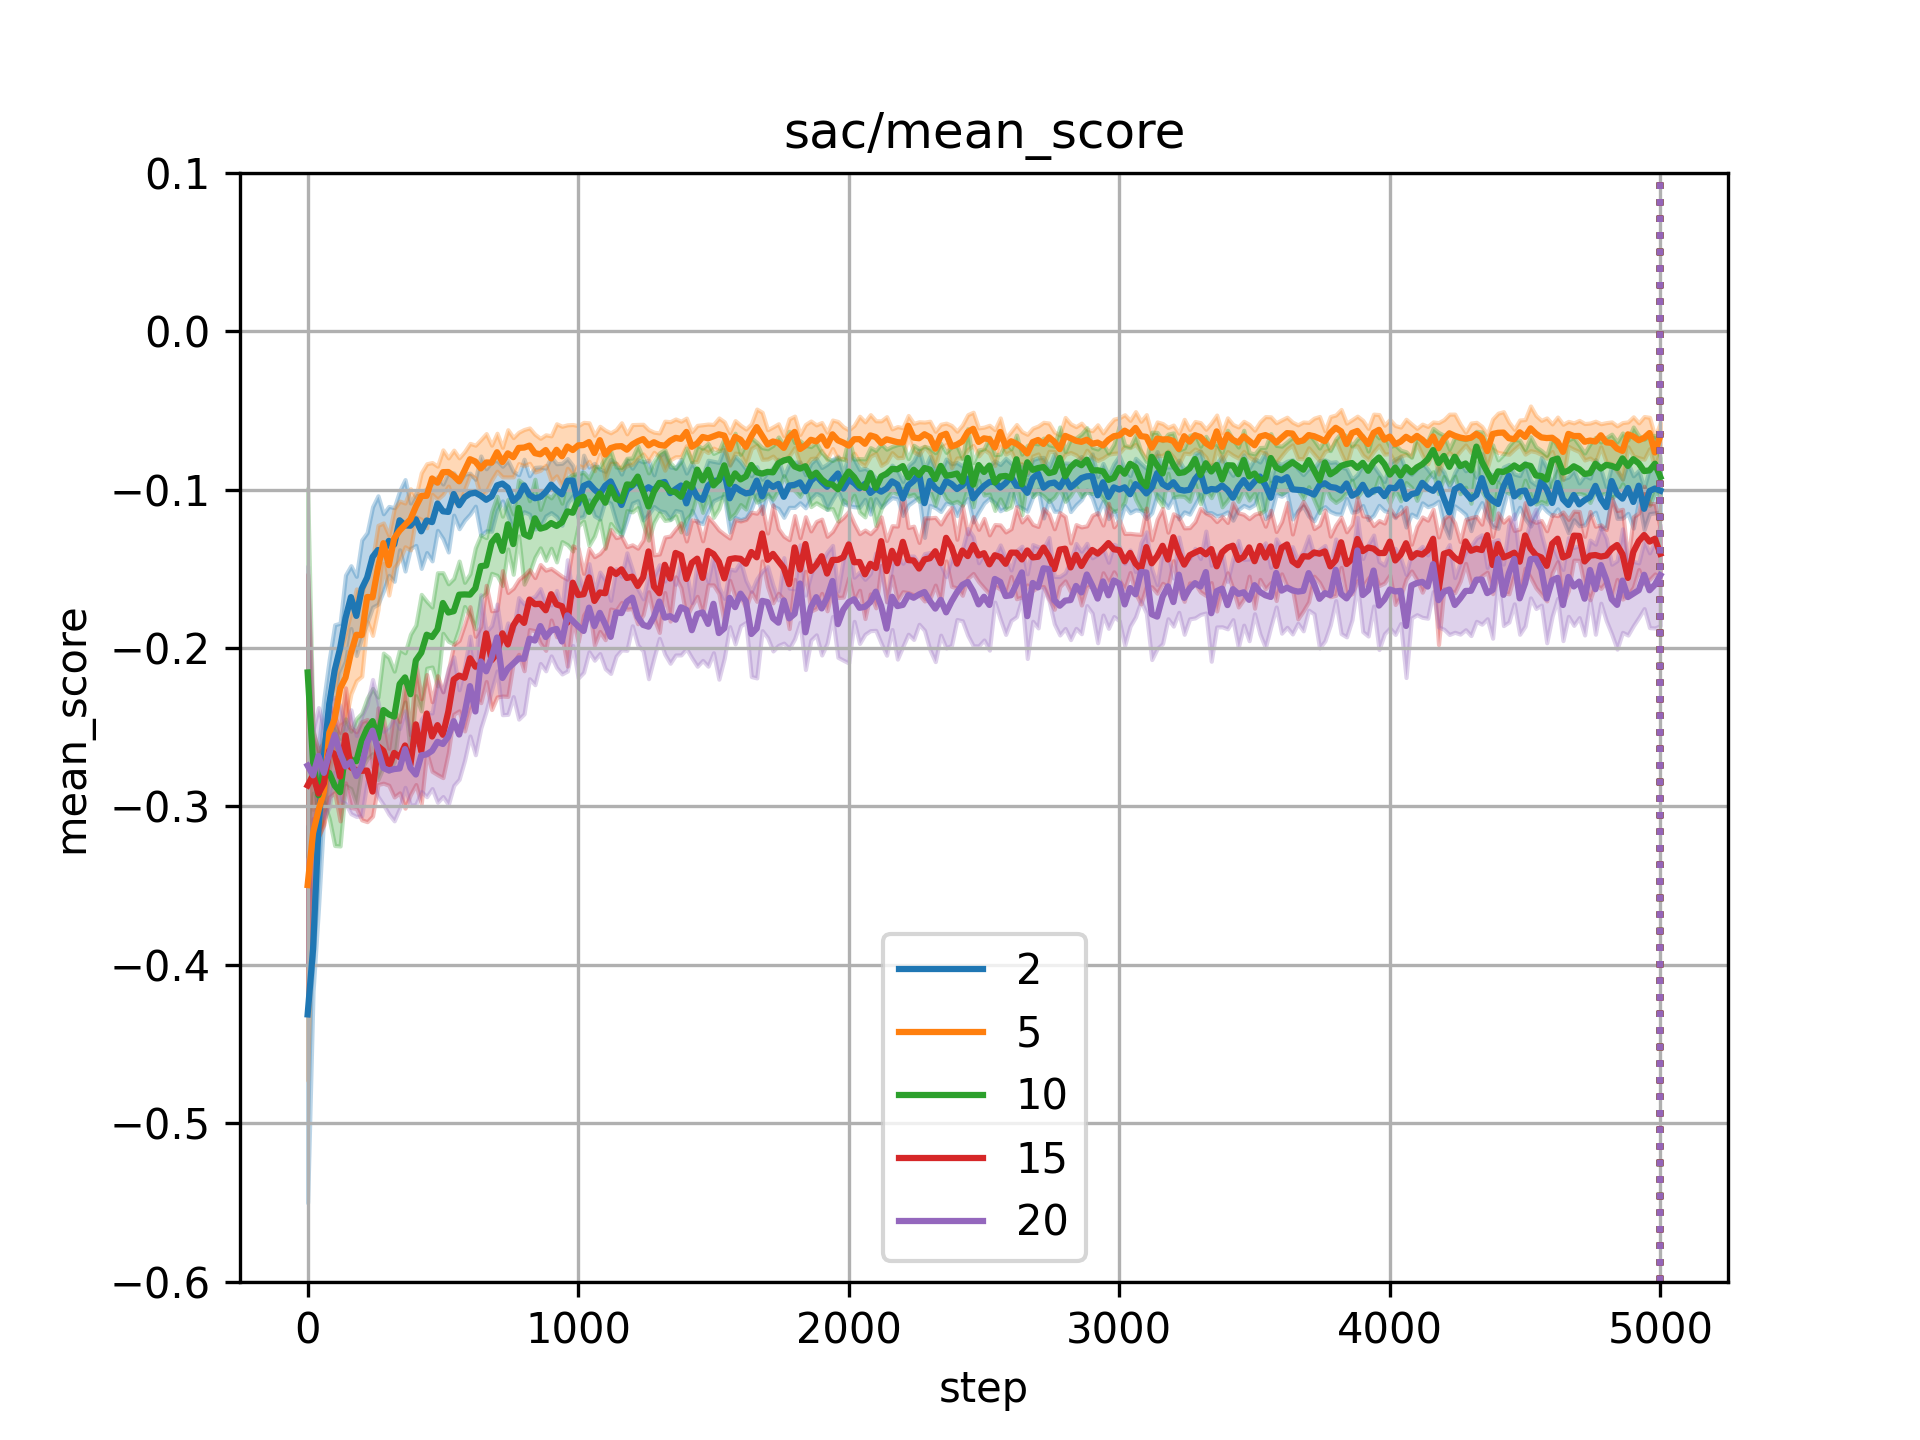
\includegraphics[width=0.46 \linewidth]{figures/experiments/sac_baseline_mean_score.png}
            \label{fig:SAC_baseline/reward}
            }
        \hfill
        \subfloat[Mean episode length over the last 20 episodes]{
        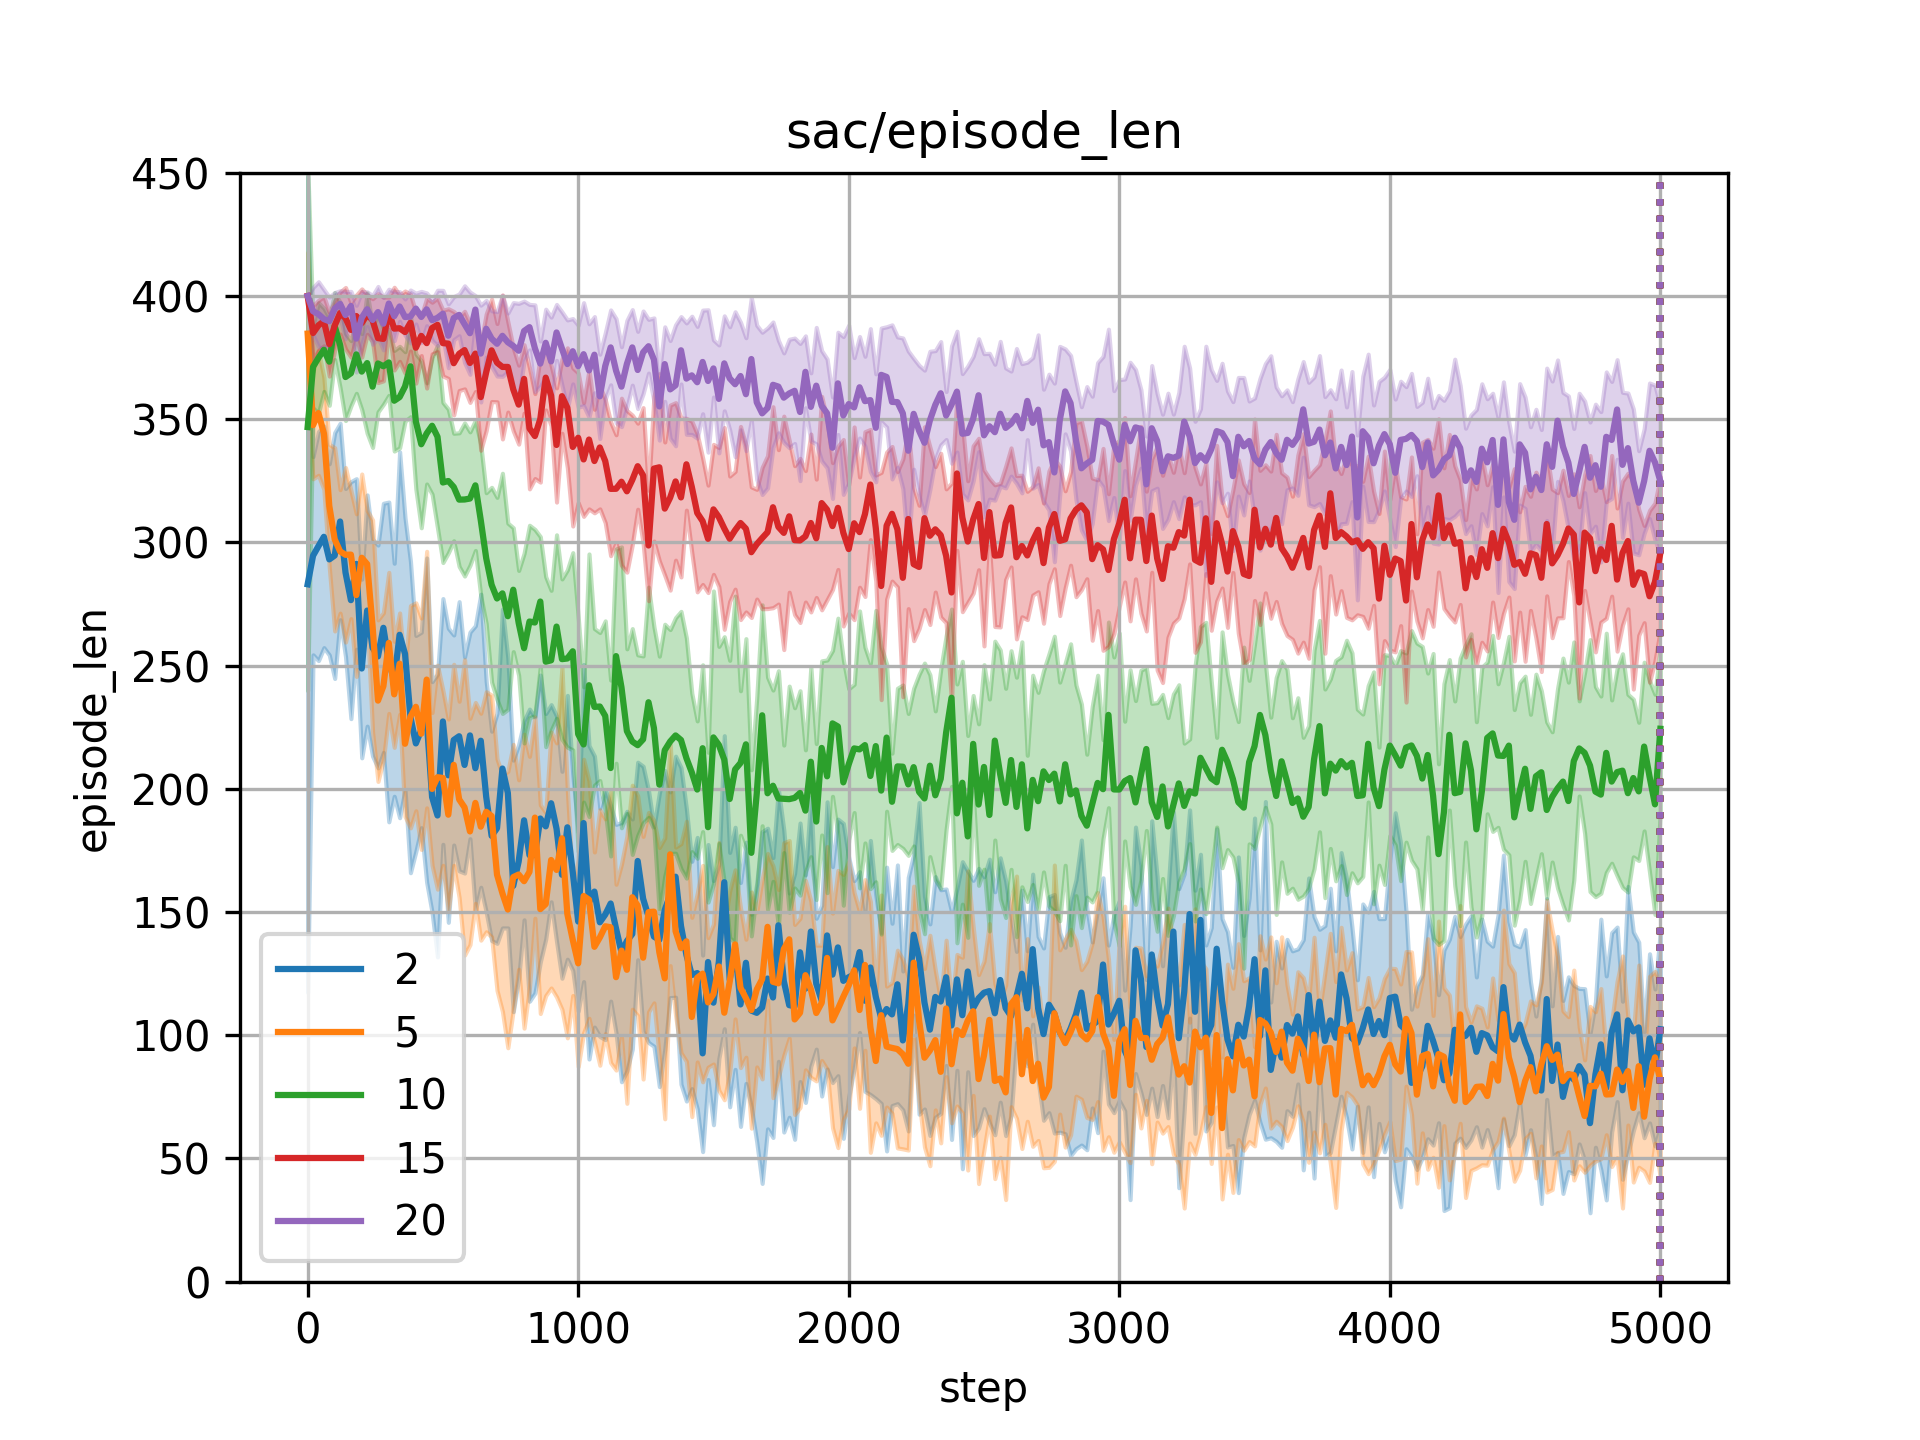
\includegraphics[width=0.46 \linewidth]{figures/experiments/sac_baseline_episode_len.png}
            \label{fig:SAC_baseline/episode_len}
            }
    \end{center}
    \caption[SAC baseline experiment results]{SAC baseline experiment results with an increasing number of joints. We can clearly see that the algorithm does not scale well with an increasing number of joints and therefor drops in performance. Each experiment was conducted 10 times and the shaded areas resemble the standard deviation around the mean.}
    \label{fig:SAC_baseline}
\end{figure}

In \figref{fig:SAC_baseline} we plotted the mean reward per step and the average episode length over the last 20 epochs for different $N \in [2, 5, 10, 15, 20]$. Overall we can observe a decrease of collected reward per step in \figref{fig:SAC_baseline/reward} and an increasing amount of steps in one episode in \figref{fig:SAC_baseline/episode_len} while increasing the number of joints $N$. In \figref{fig:SAC_baseline/episode_len} the training curves are approaching the maximum step limit of one episode while increasing the number of joints. Additionally we can observe that the standard deviation over multiple experiments is decreasing while increasing the number of joints.

To show the actual behavior of an agent in a standardized setting we also plot an inference episode in \figref{fig:SAC_baseline_inference_trajectory} and the distance remaining to target in \figref{fig:SAC_baseline_inference_distance}. The standardization in \figref{fig:SAC_baseline_inference_trajectory} for one selected experiment for a relative consistent target position at $[-0.5, 0.5] \cdot N$. \\
As expected from the performance statistics in \figref{fig:SAC_baseline} agents with two and five joints perform much better than agents with ten or more joints. \\
Interesting to observe is that all agents are minimizing the distance to the target quite fast in their first couple of steps. But after missing the target closely the agents behavior starts to oscillate.
For closer inspection please refer to \figref{fig:SAC_baseline_inference_trajectory/greedy_15} and \figref{fig:SAC_baseline_inference_trajectory/greedy_20}. 


\begin{figure}
    \begin{center}
        \subfloat[From experiment 2\textunderscore 1691621262.]{
            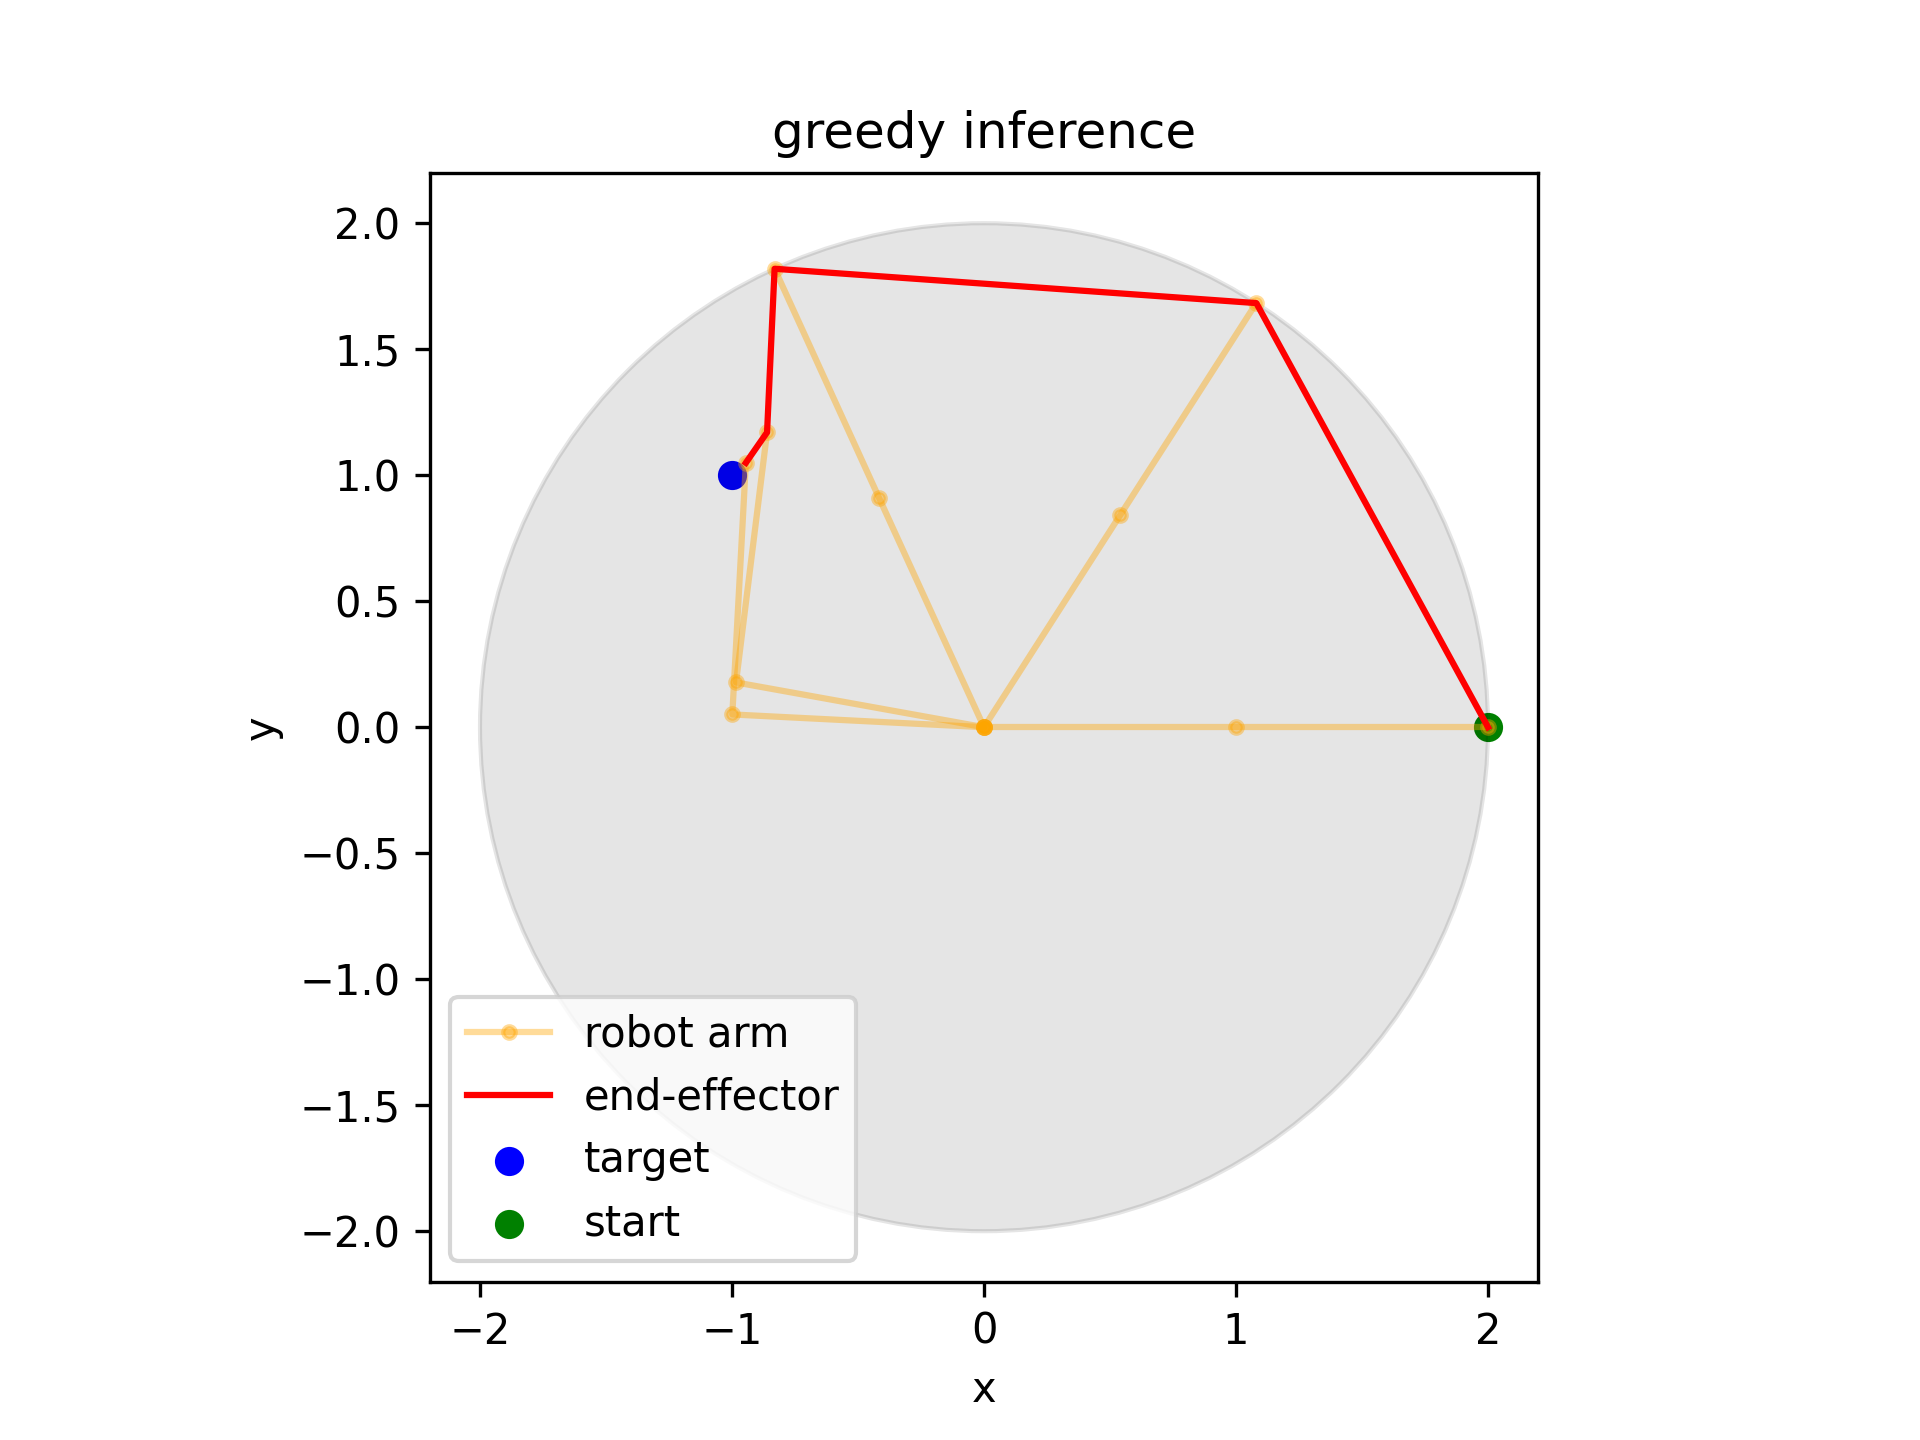
\includegraphics[width=0.31 \linewidth]{figures/experiments/greedy_inference_baseline_2_1691621262_5000.png}
            \label{fig:SAC_baseline_inference_trajectory/greedy_2}
            }
        \hfill
        \subfloat[From experiment 5\textunderscore 1691624939. To make things more clear only every 5th robot arm is drawn]{
            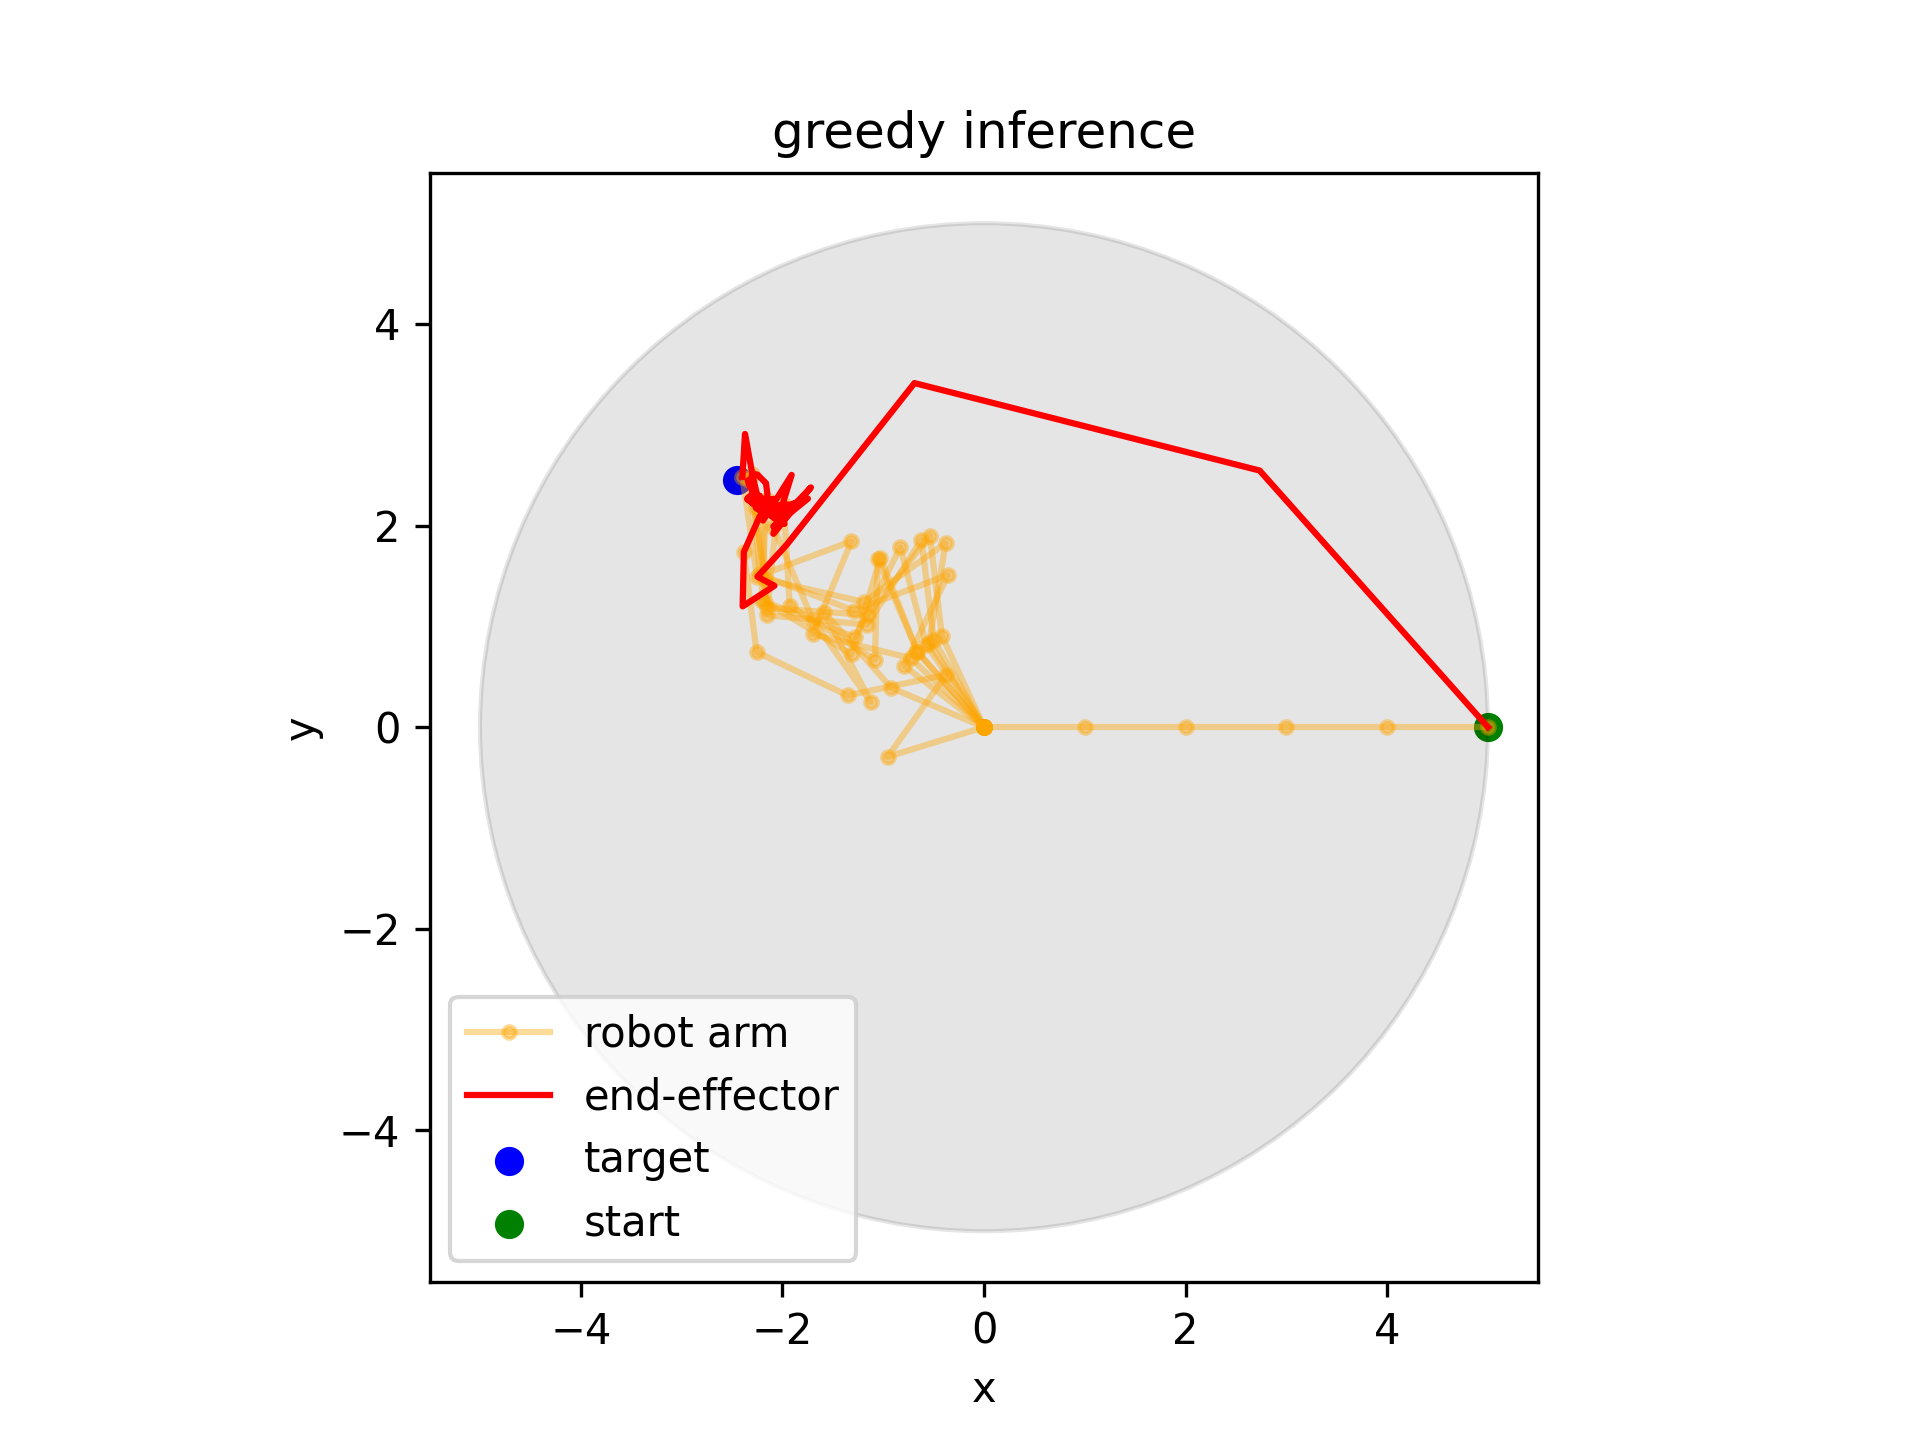
\includegraphics[width=0.31 \linewidth]{figures/experiments/greedy_inference_baseline_5_1691624939_5000.png}
            \label{fig:SAC_baseline_inference_trajectory/greedy_5}
            }
        \hfill
        \subfloat[From experiment 10\textunderscore 1691622498. To make things more clear only every 5th robot arm is drawn]{
            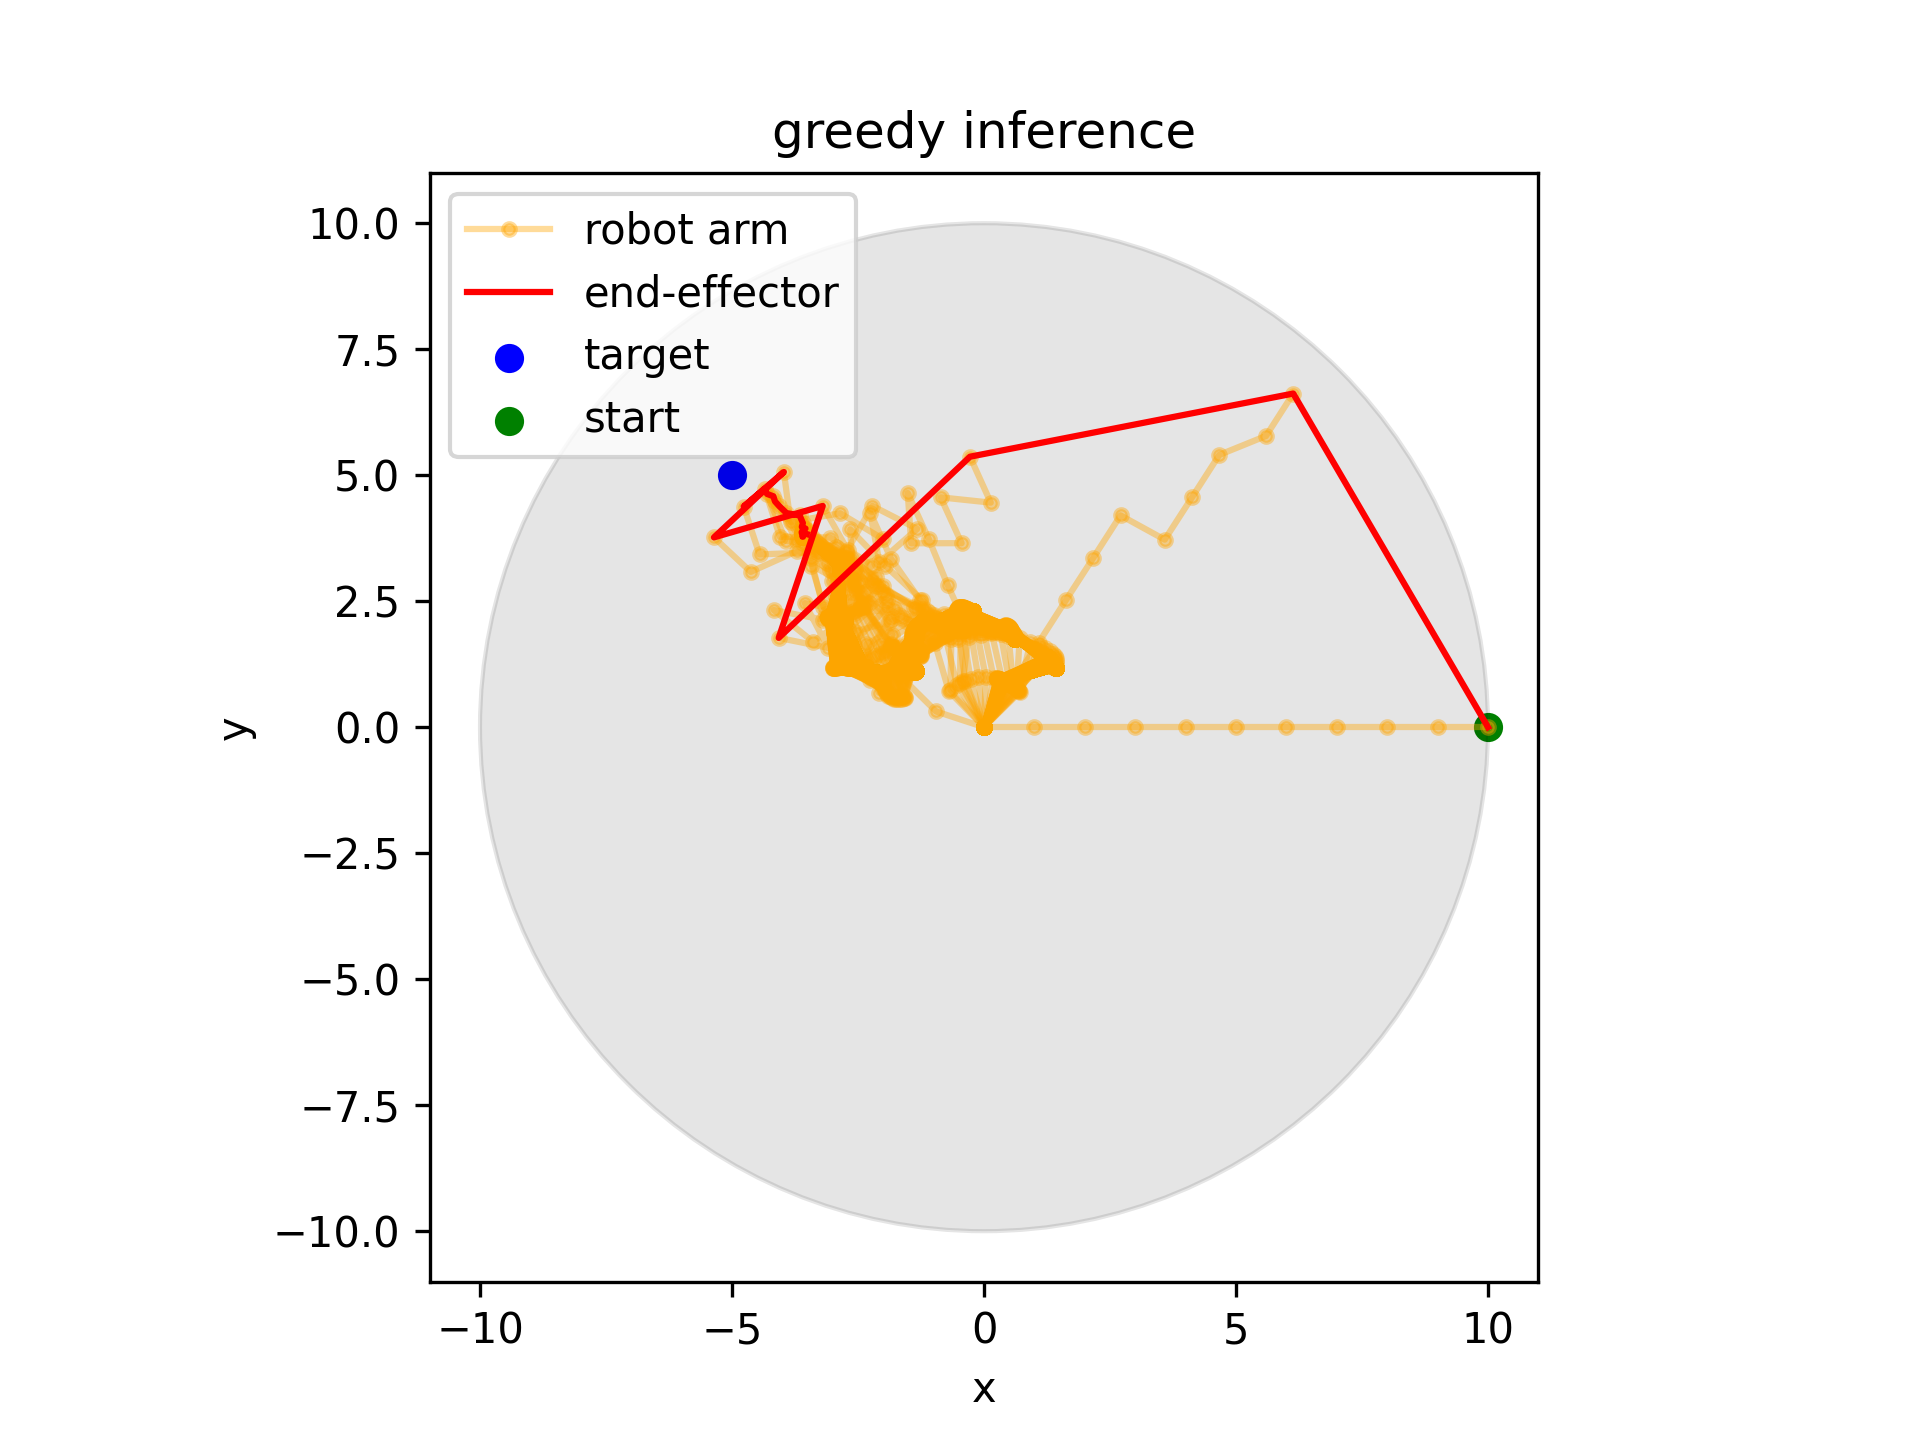
\includegraphics[width=0.31 \linewidth]{figures/experiments/greedy_inference_baseline_10_1691622498_5000.png}
            \label{fig:SAC_baseline_inference_trajectory/greedy_10}
            }
        \\
        \subfloat[From experiment 15\textunderscore 1691619106. To make things more clear only every 40th robot arm is drawn]{
            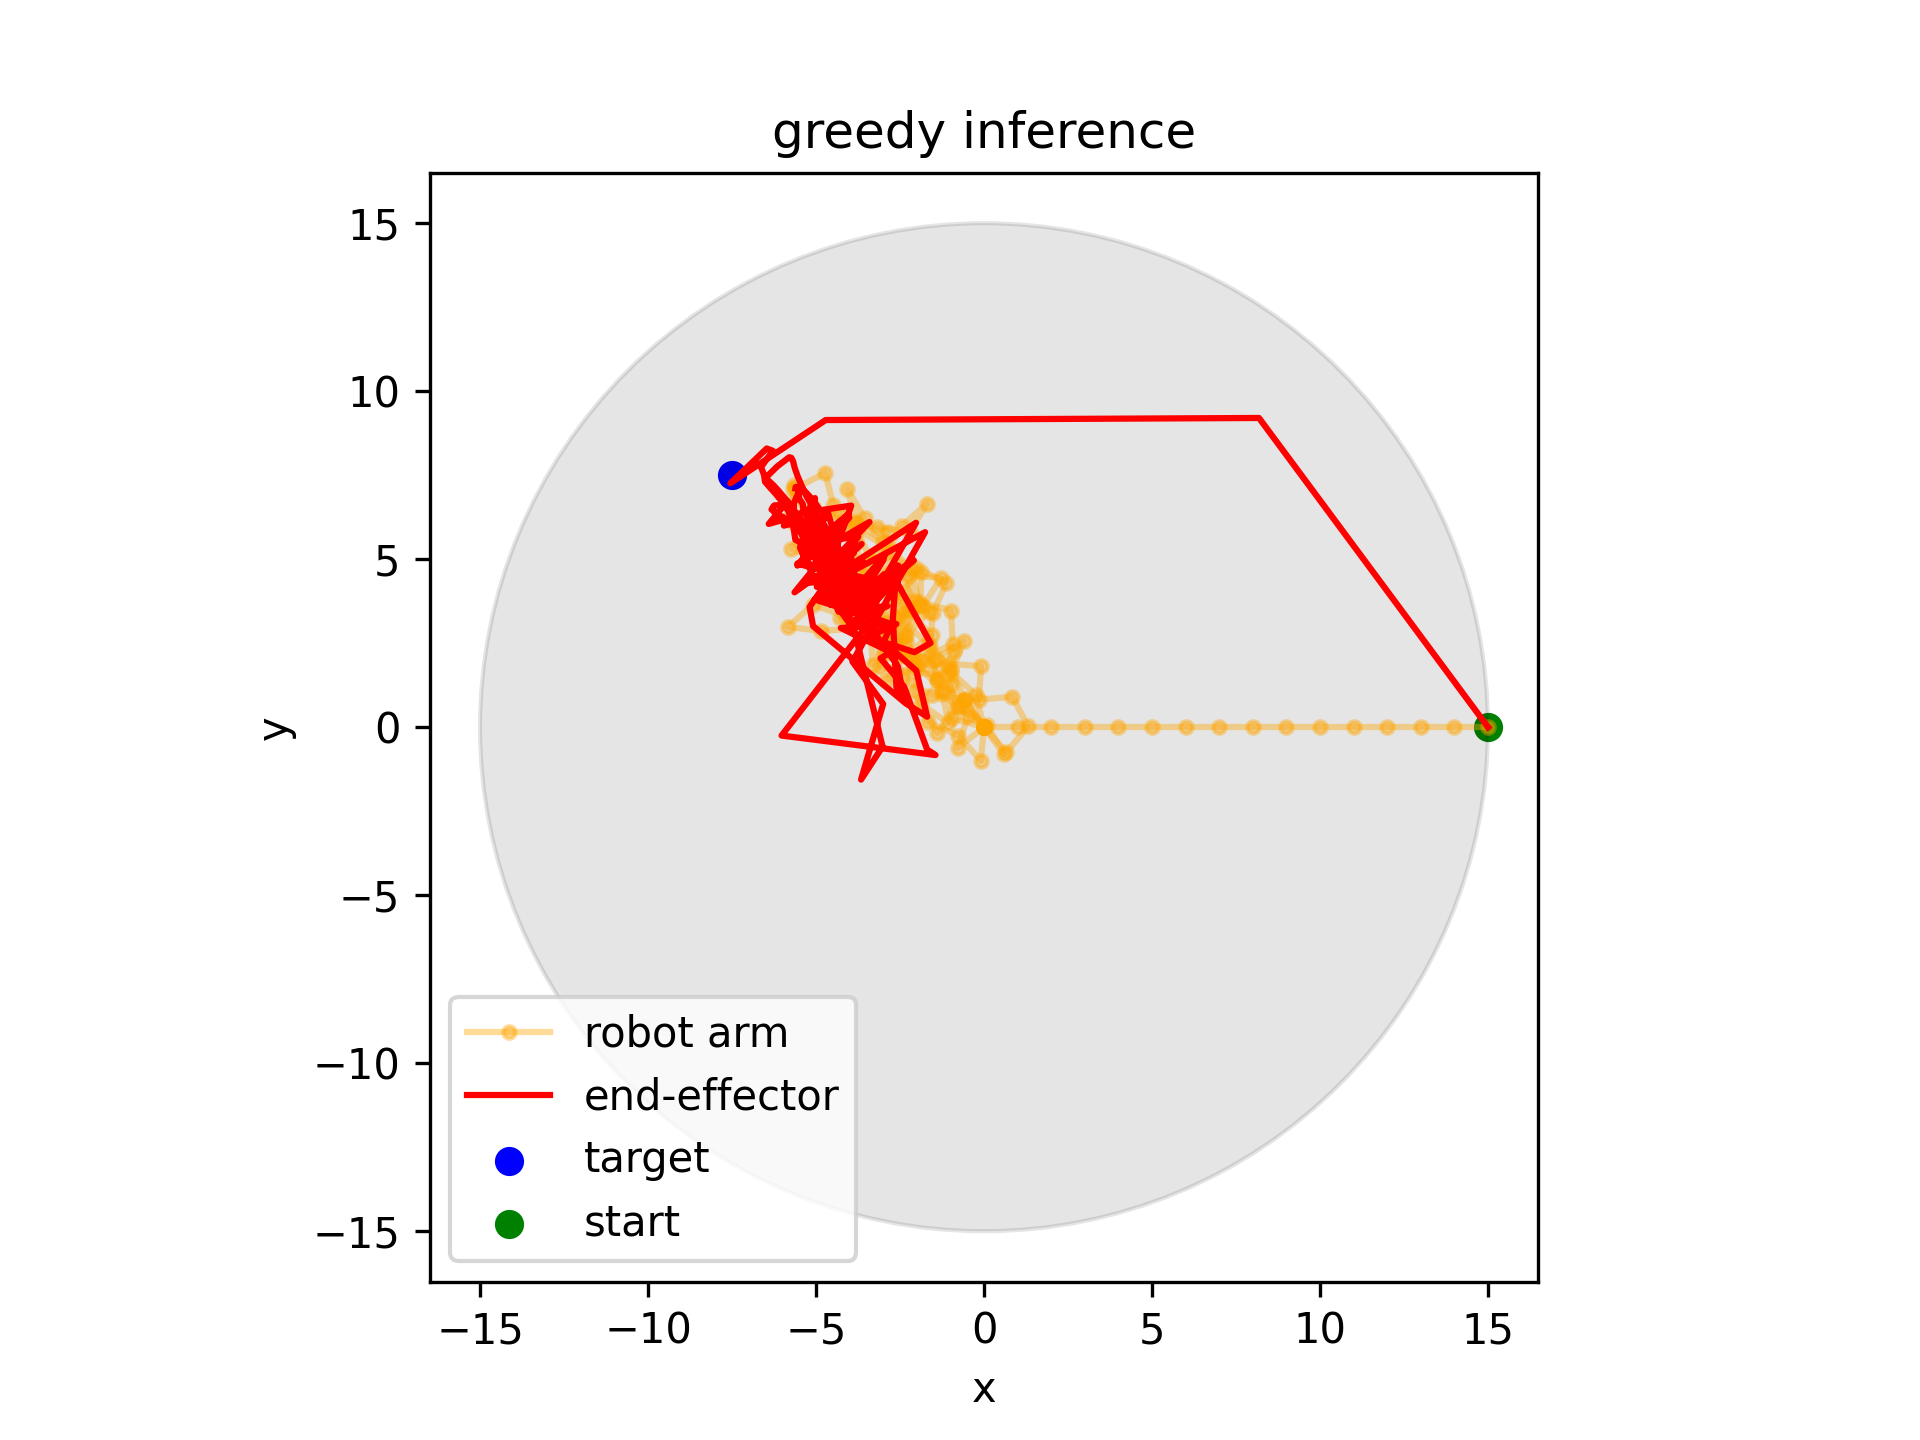
\includegraphics[width=0.31 \linewidth]{figures/experiments/greedy_inference_baseline_15_1691619106_5000.png}
            \label{fig:SAC_baseline_inference_trajectory/greedy_15}
            }
        \subfloat[From experiment 20\textunderscore 1691619159. To make things more clear only every 40th robot arm is drawn]{
            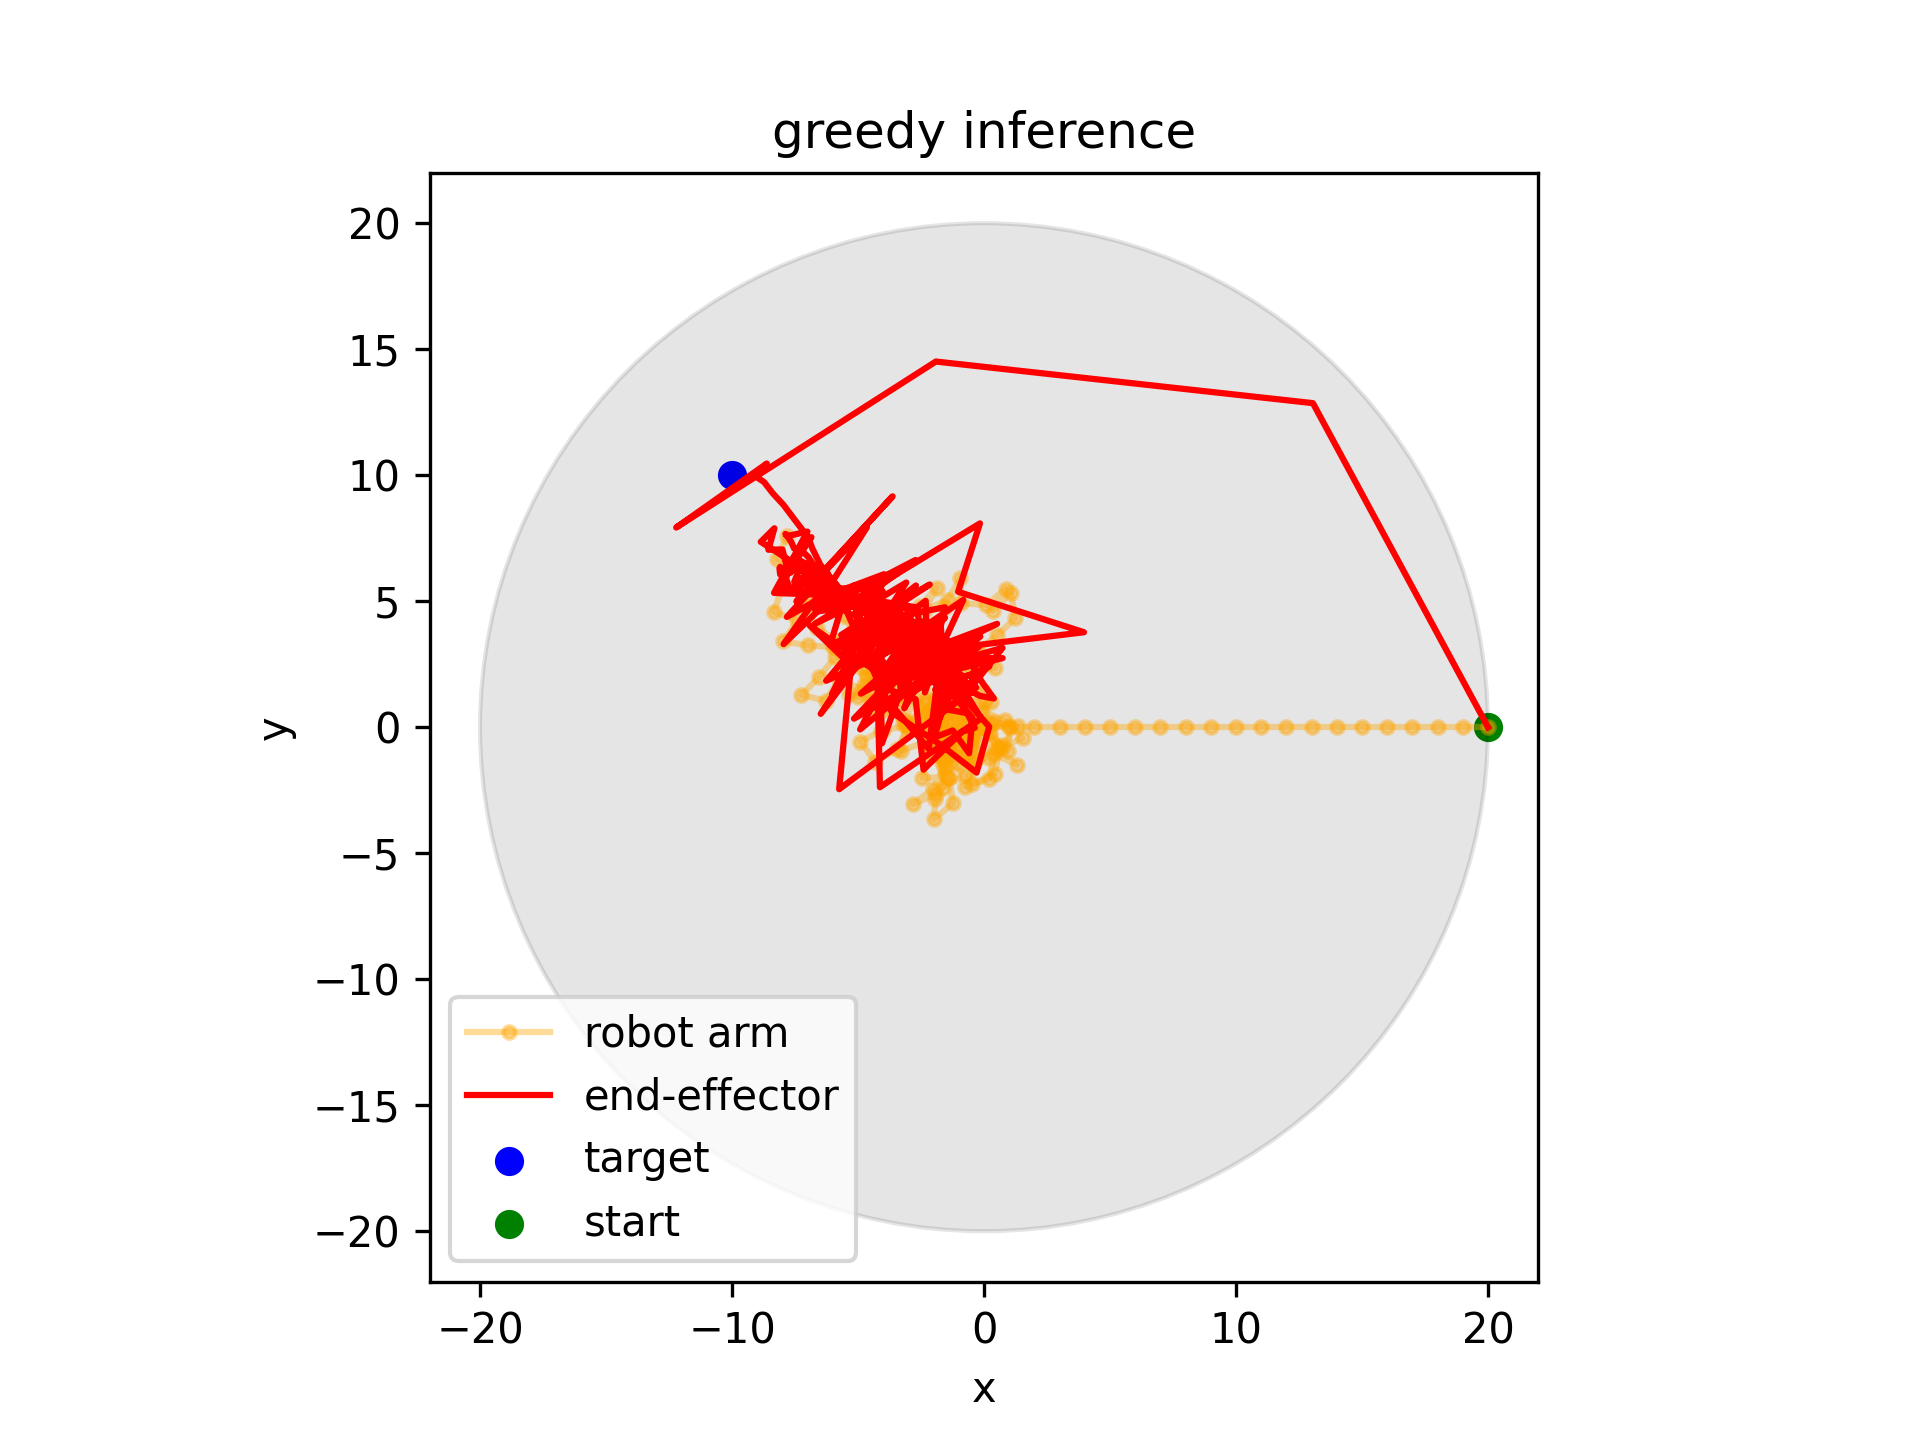
\includegraphics[width=0.31 \linewidth]{figures/experiments/greedy_inference_baseline_20_1691619159_5000.png}
            \label{fig:SAC_baseline_inference_trajectory/greedy_20}
            }
    \end{center}
    \caption[SAC baseline inference]{SAC inference. The trajectory is plotted in red. robot arms are drawn in yellow with the little dots as positions of each joint. Target position and start position are scattered in blue and green. The space an end-effector is able to reach is plotted in grey.}
    \label{fig:SAC_baseline_inference_trajectory}
\end{figure}
\begin{figure}
    \begin{center}
        \subfloat[Experiment 2\textunderscore 1691621262.]{
        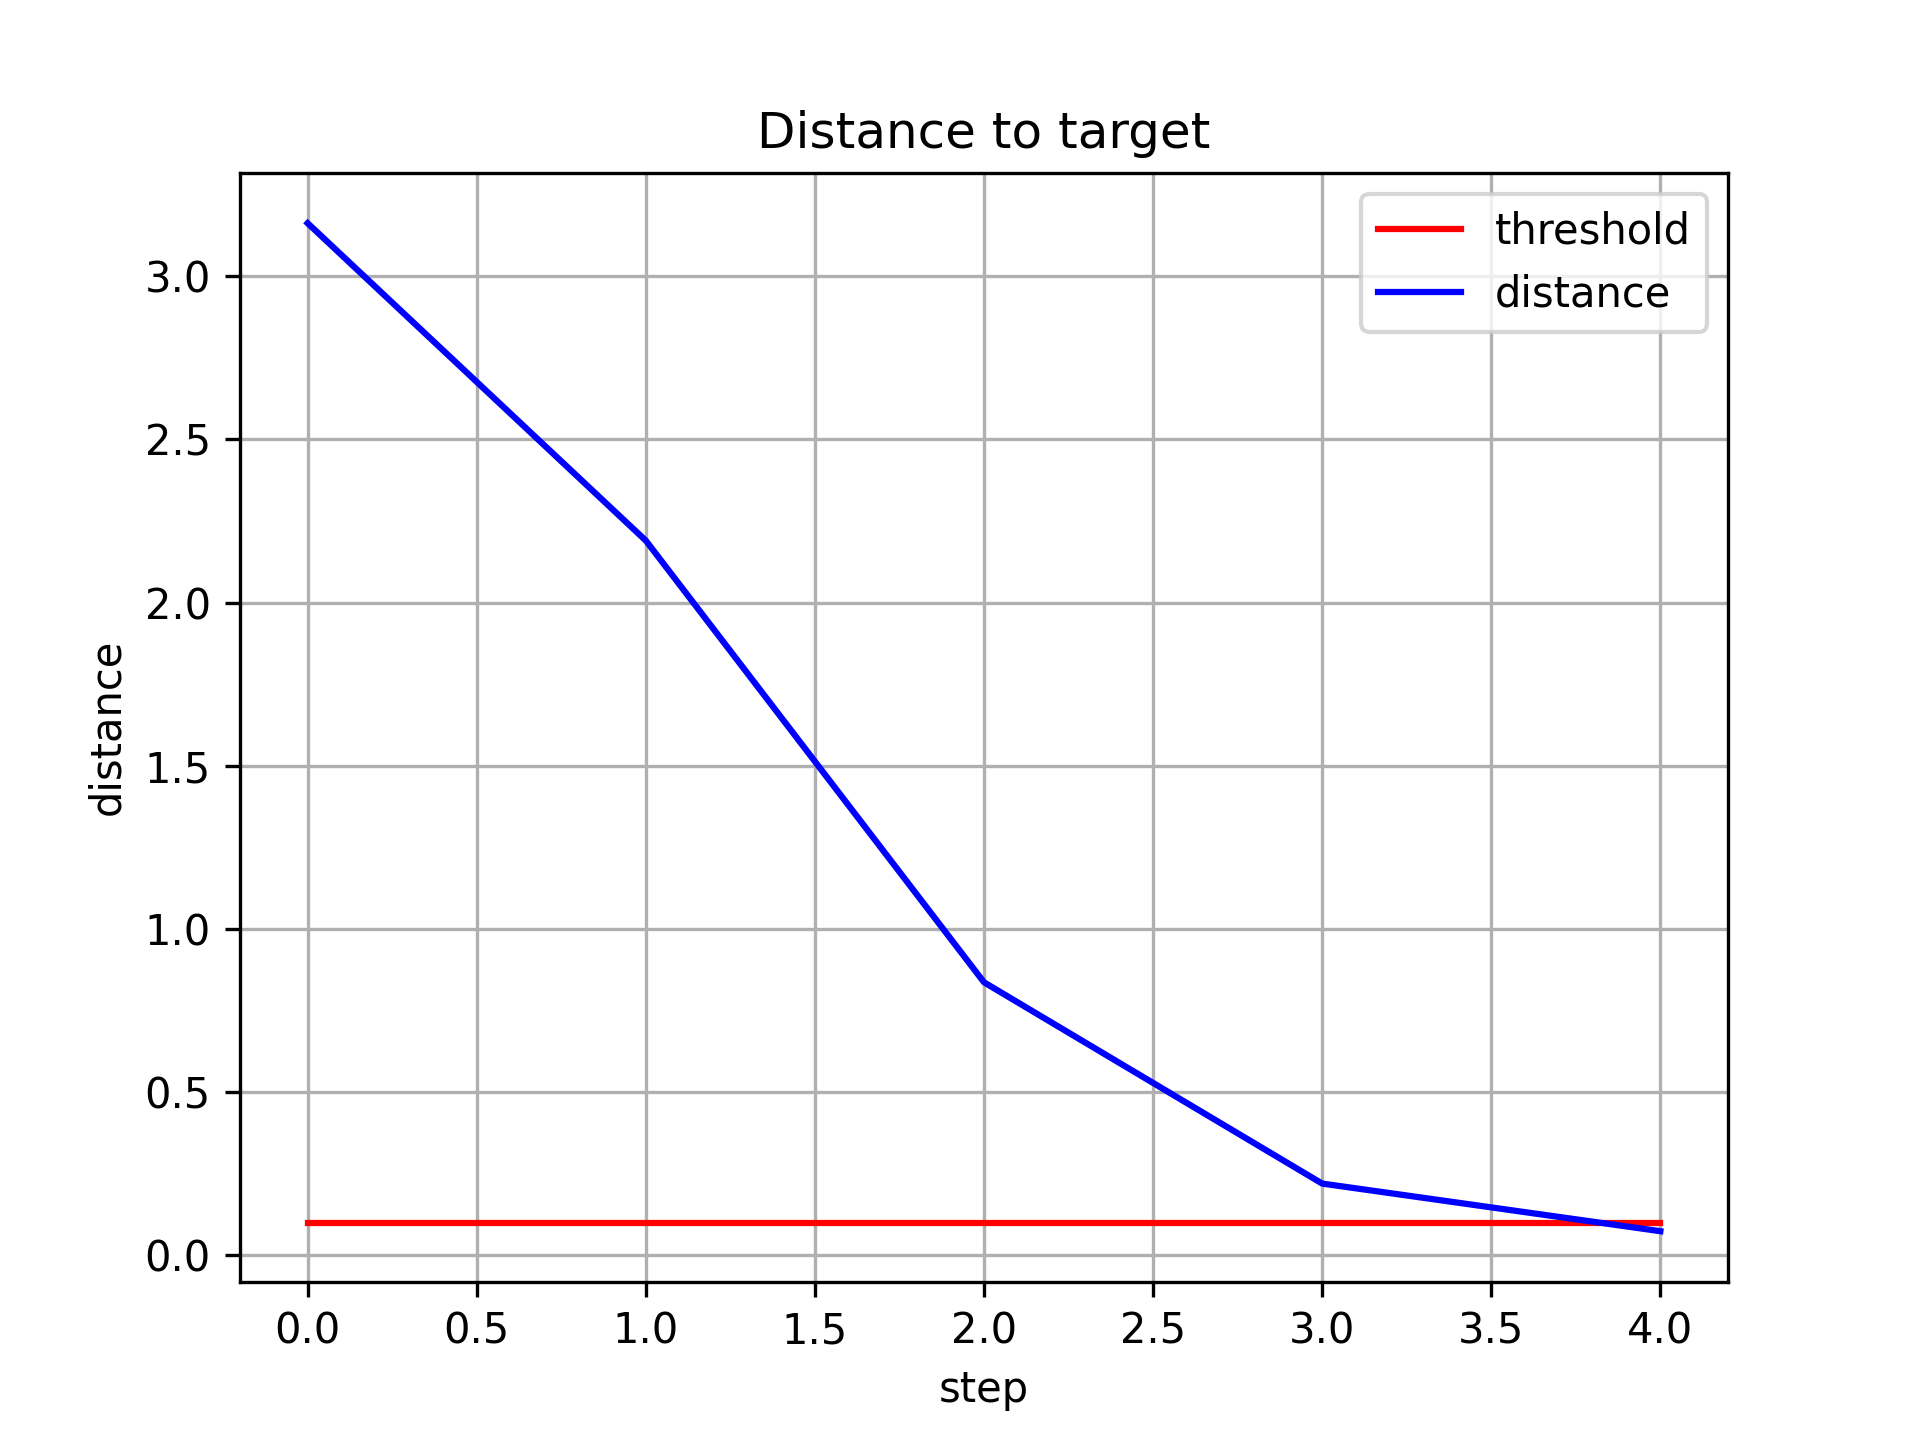
\includegraphics[width=0.31 \linewidth]{figures/experiments/Distance_to_target_baseline_2_1691621262_5000.png}
            \label{fig:SAC_baseline_inference/distance_2}
            }
        \hfill
        \subfloat[Experiment 5\textunderscore 1691624939 ]{
        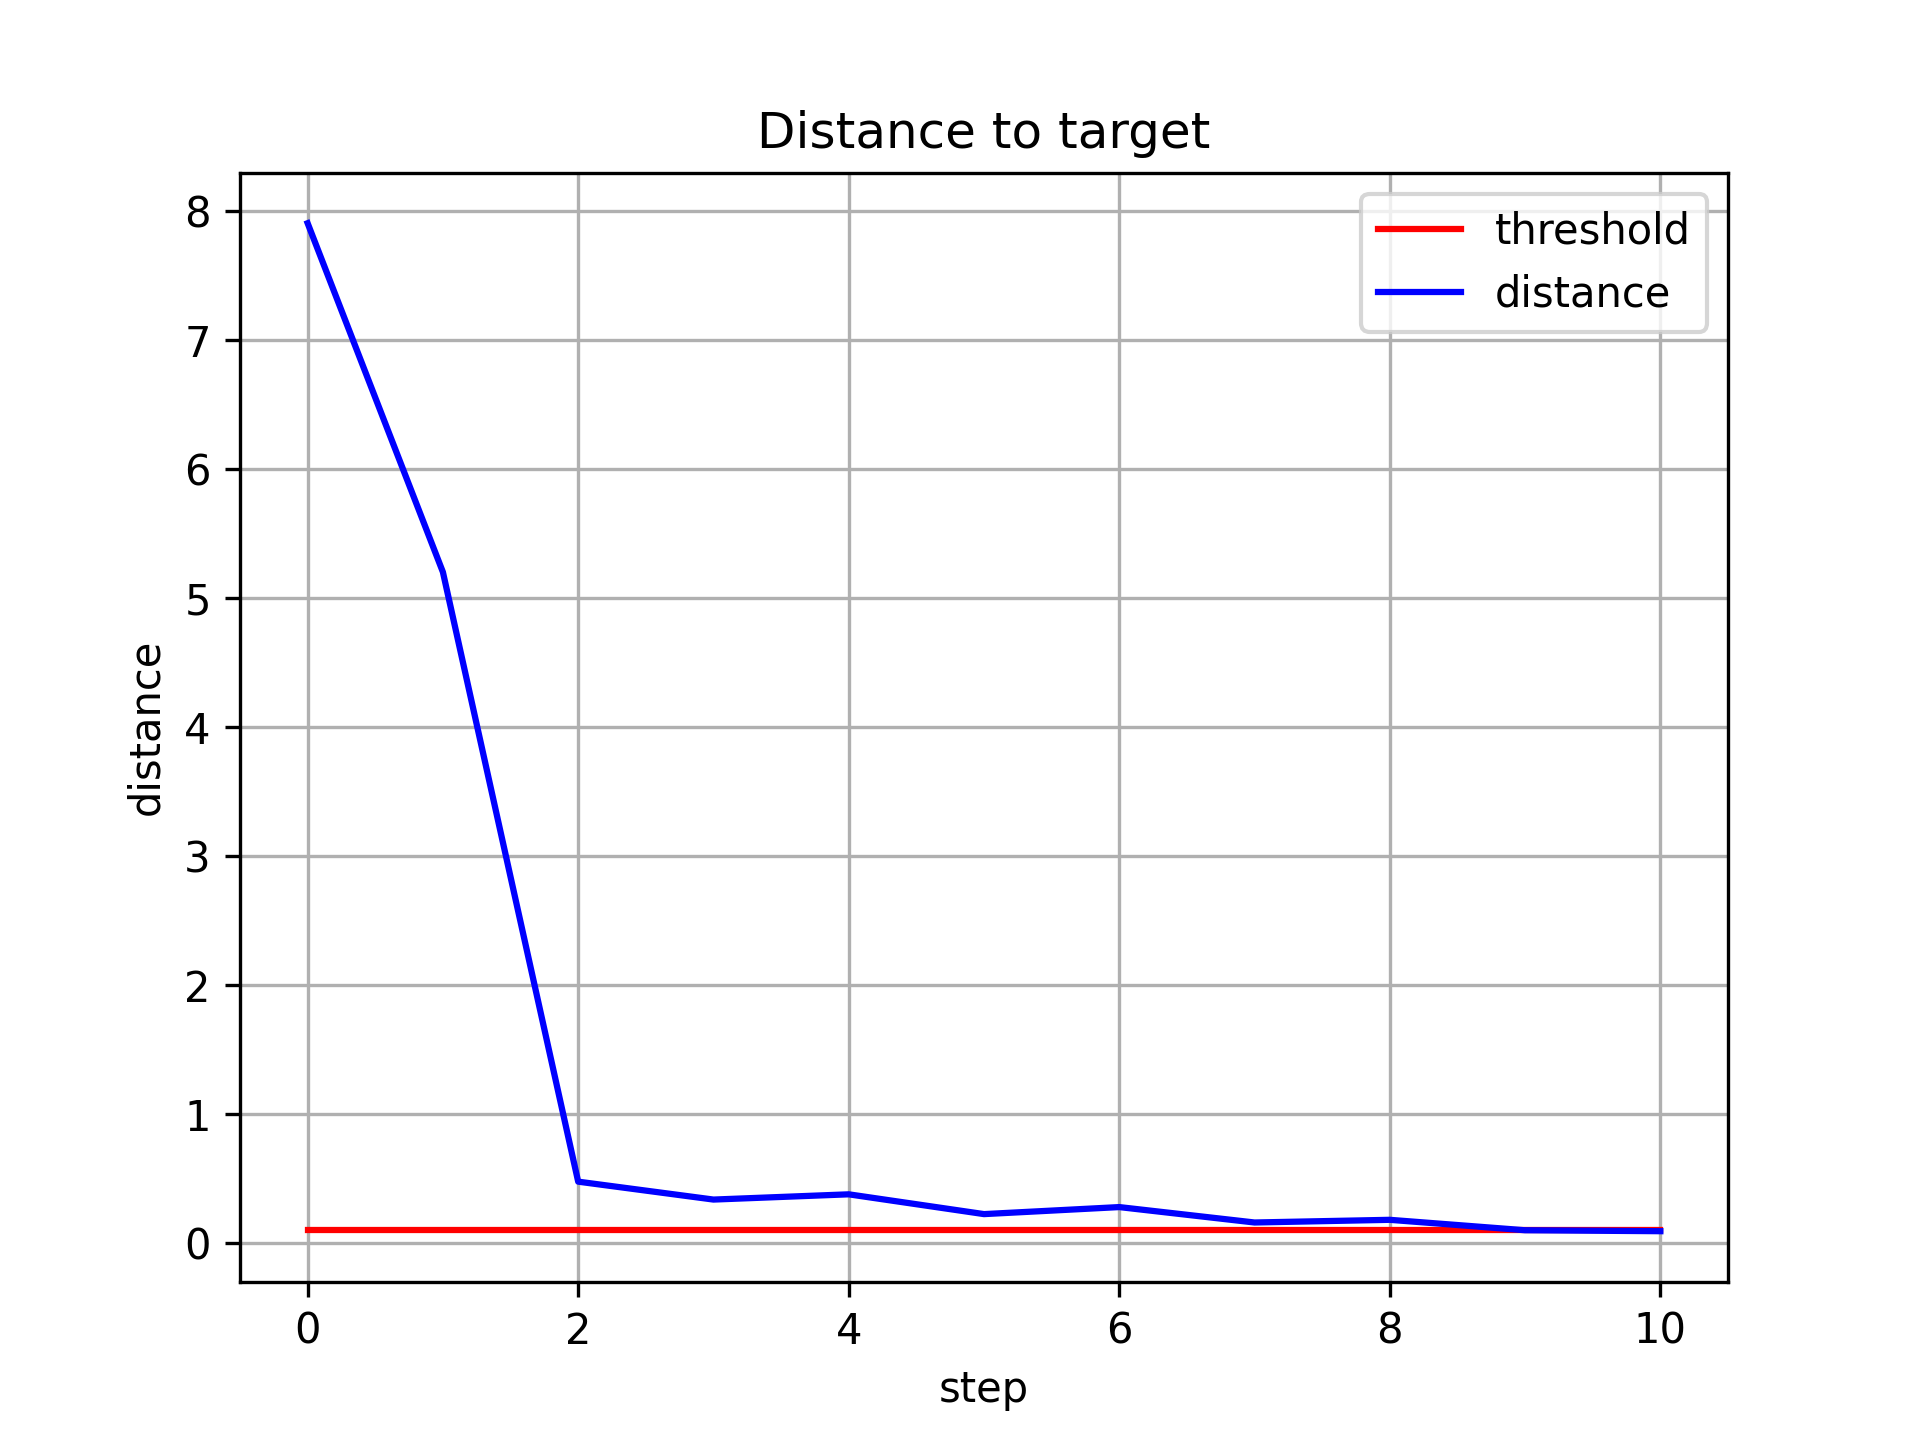
\includegraphics[width=0.31 \linewidth]{figures/experiments/Distance_to_target_baseline_5_1691624939_5000.png}
            \label{fig:SAC_baseline_inference/distance_5}
            }
        \hfill
        \subfloat[Experiment 10\textunderscore 1691622498 ]{
        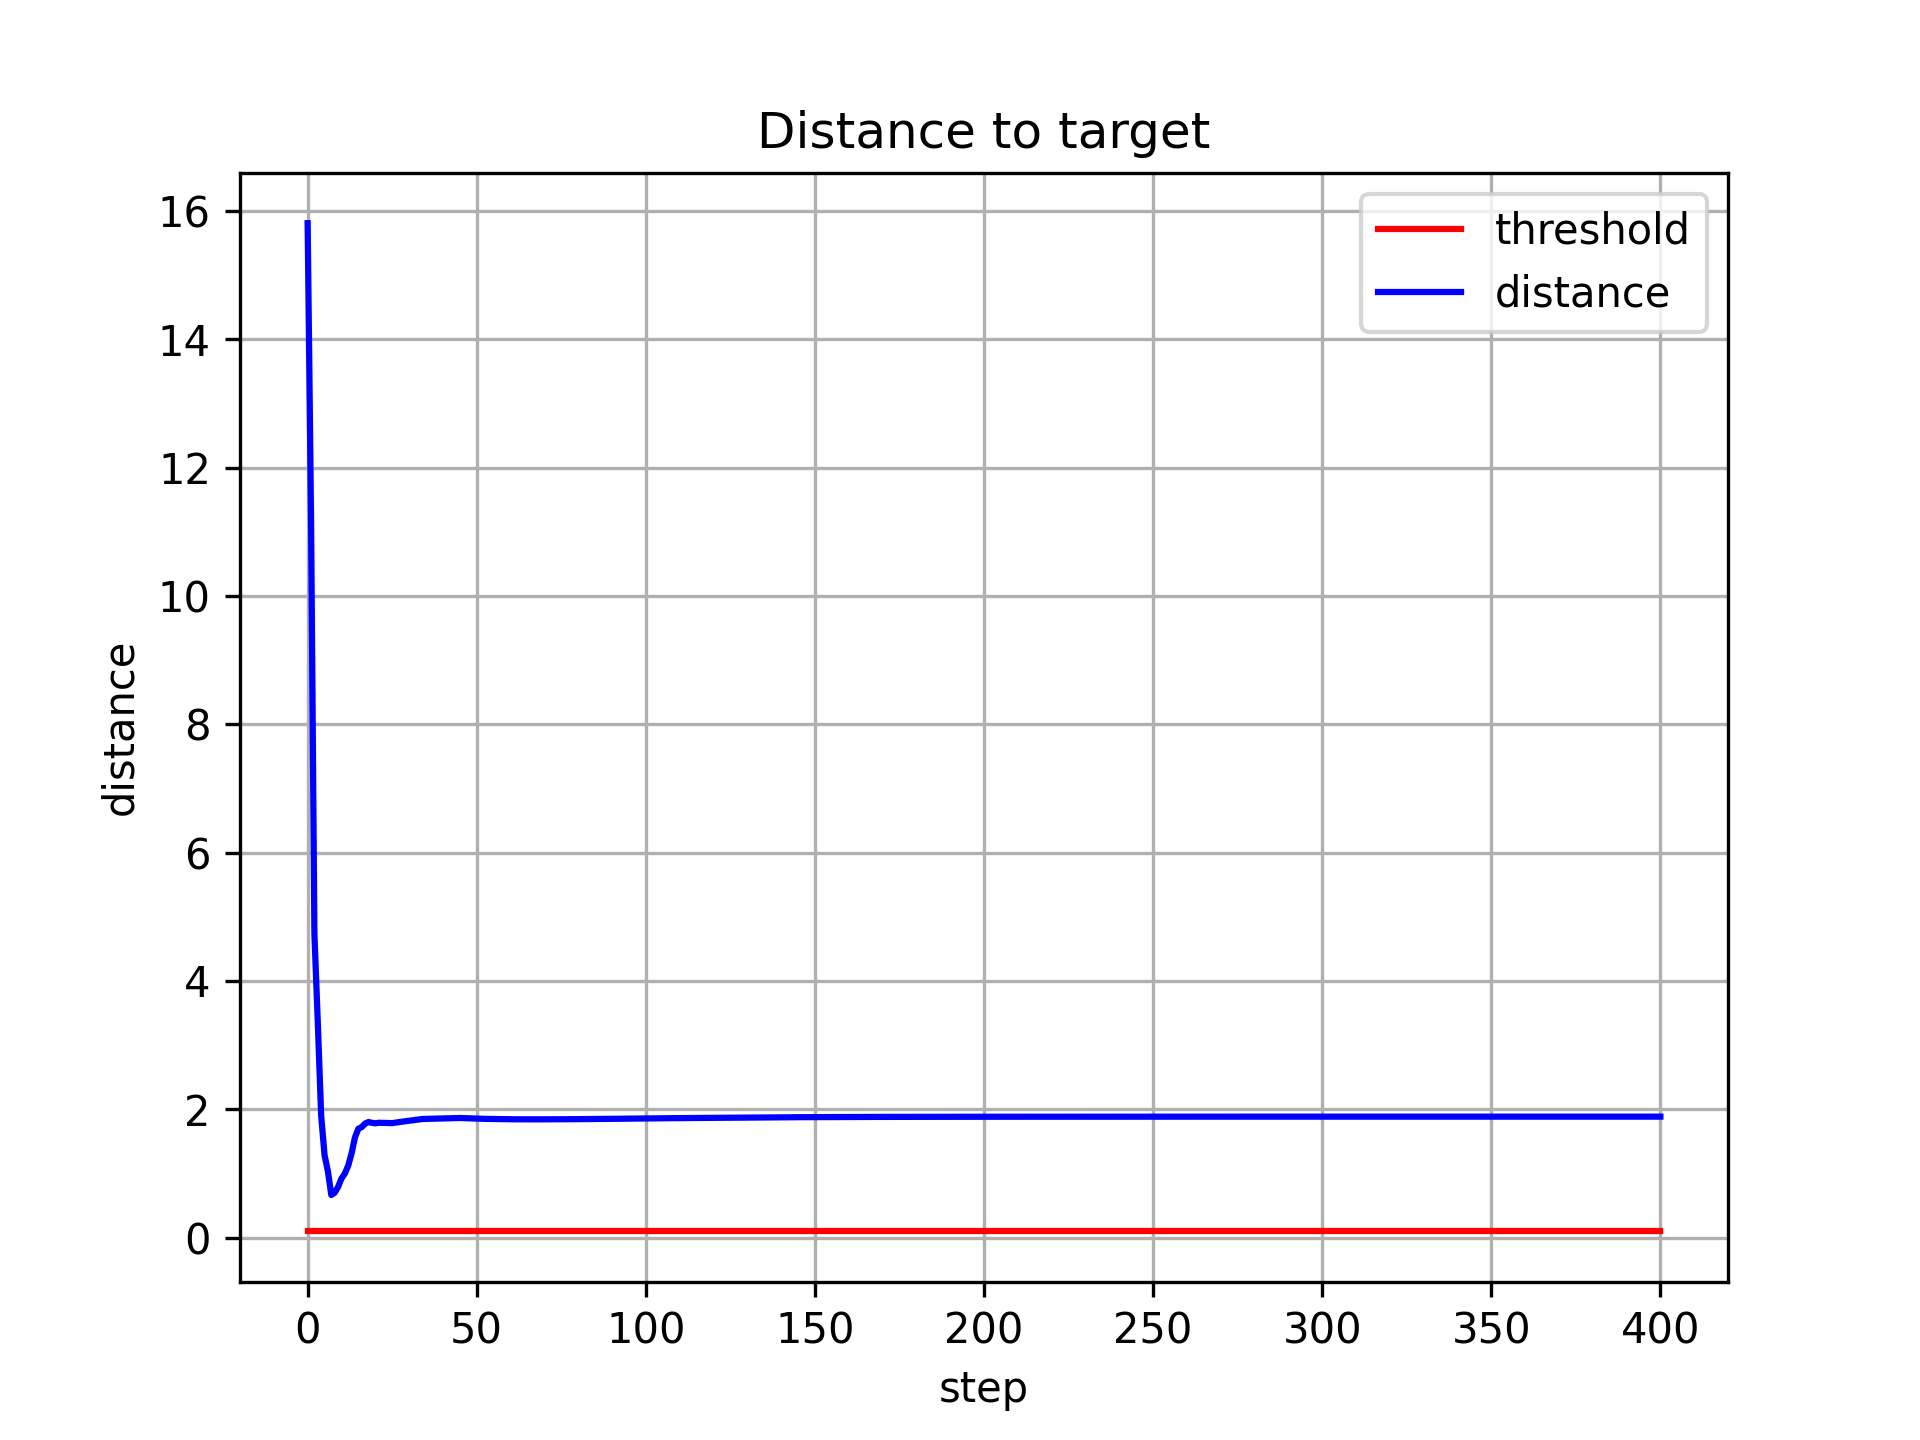
\includegraphics[width=0.31 \linewidth]{figures/experiments/Distance_to_target_baseline_10_1691622498_5000.png}
            \label{fig:SAC_baseline_inference/distance_10}
            }
        \\
        \subfloat[Experiment 15\textunderscore 1691619106 ]{
        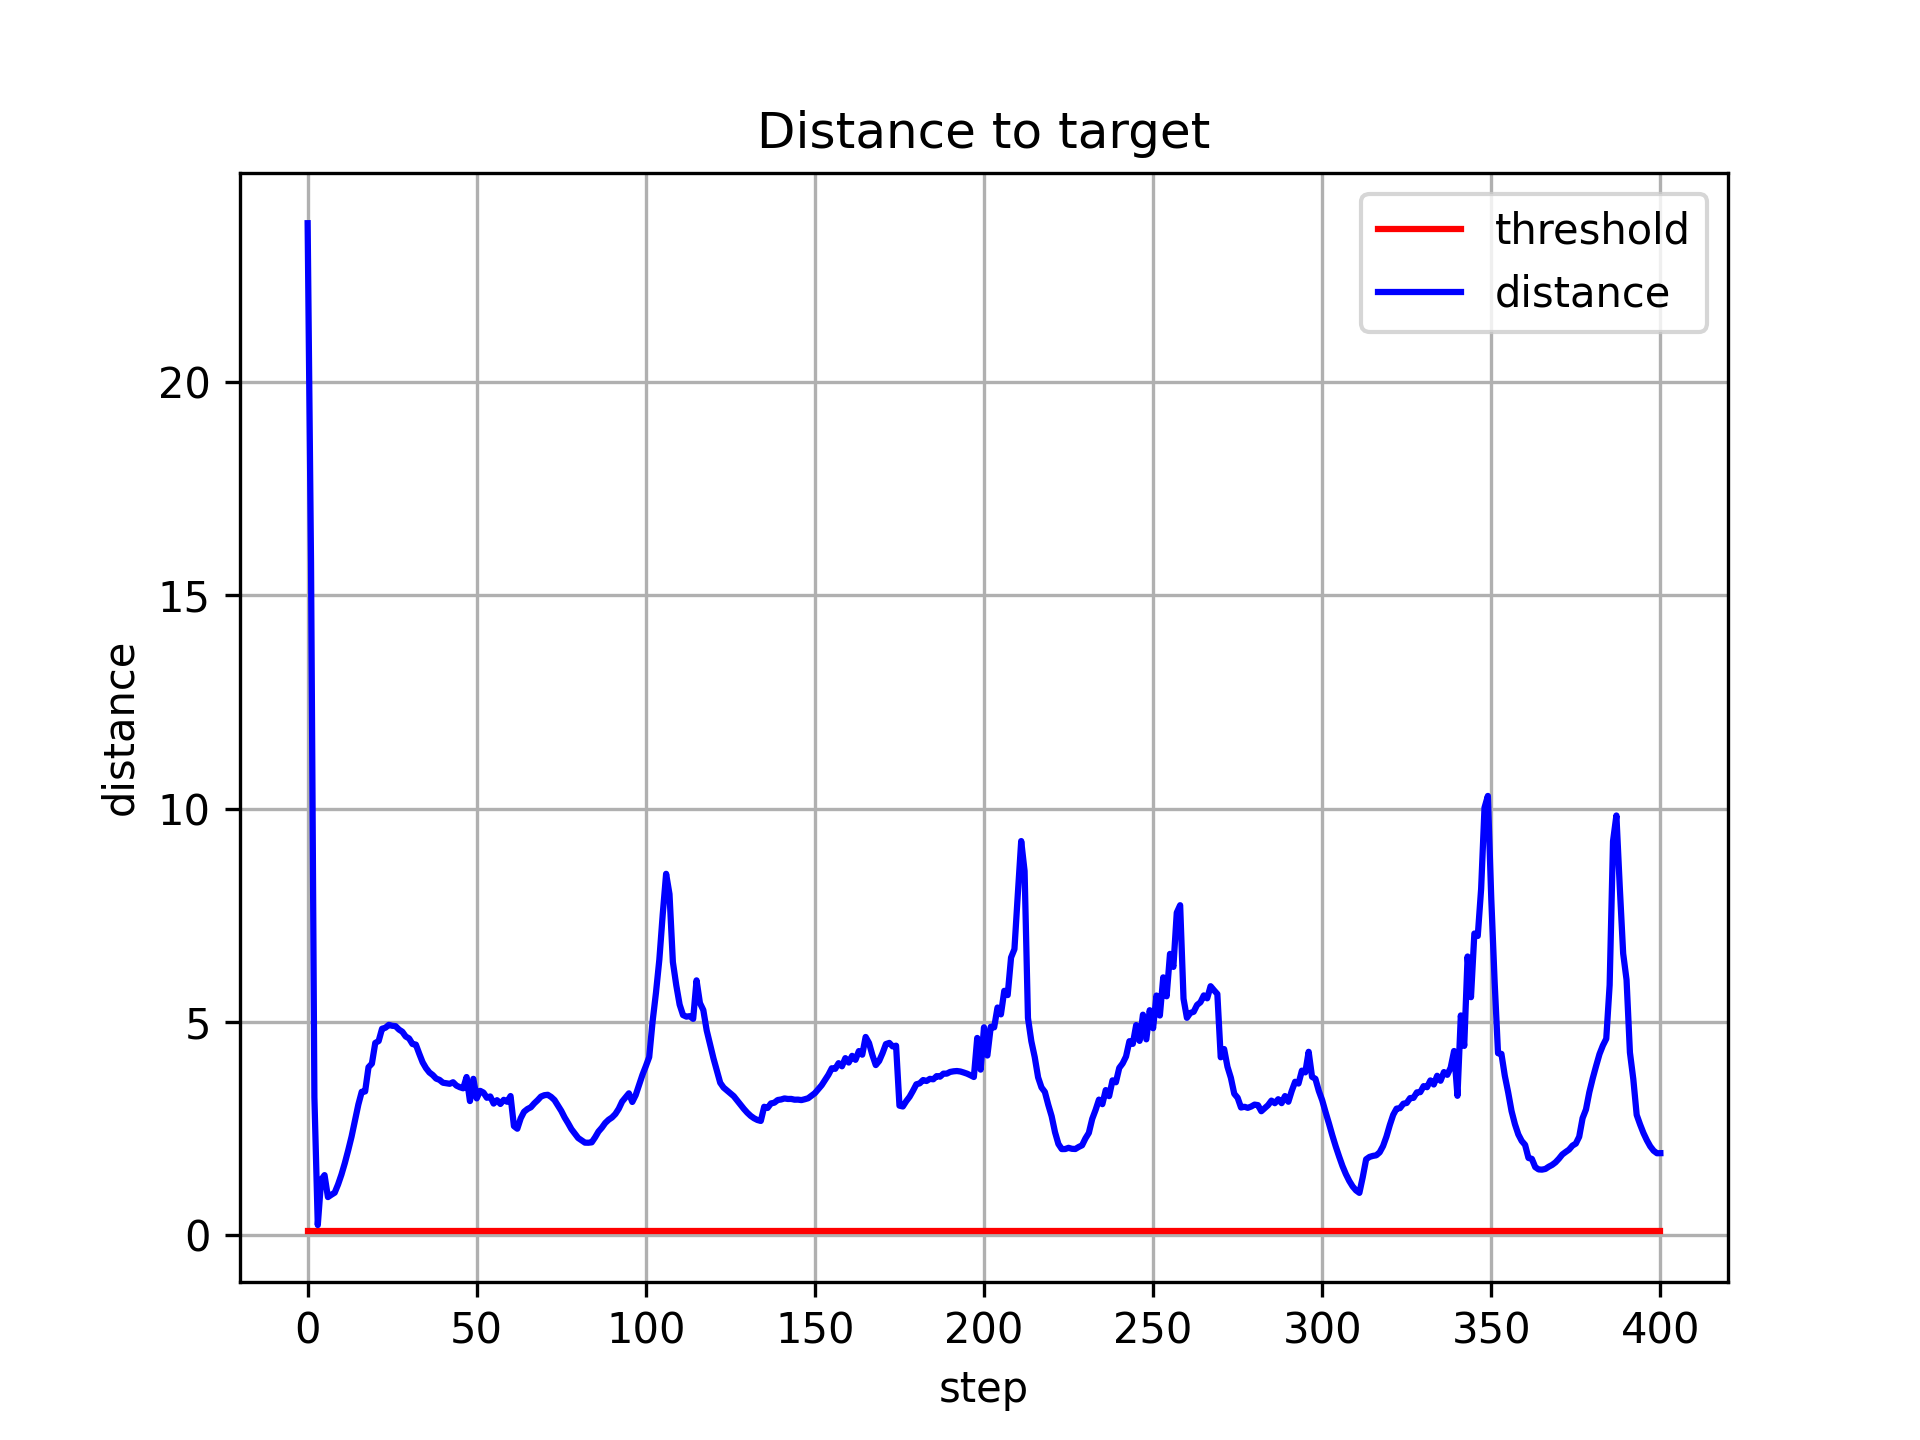
\includegraphics[width=0.31 \linewidth]{figures/experiments/Distance_to_target_baseline_15_1691619106_5000.png}
            \label{fig:SAC_baseline_inference/distance_15}
            }
        \subfloat[Experiment 20\textunderscore 1691619159 ]{
        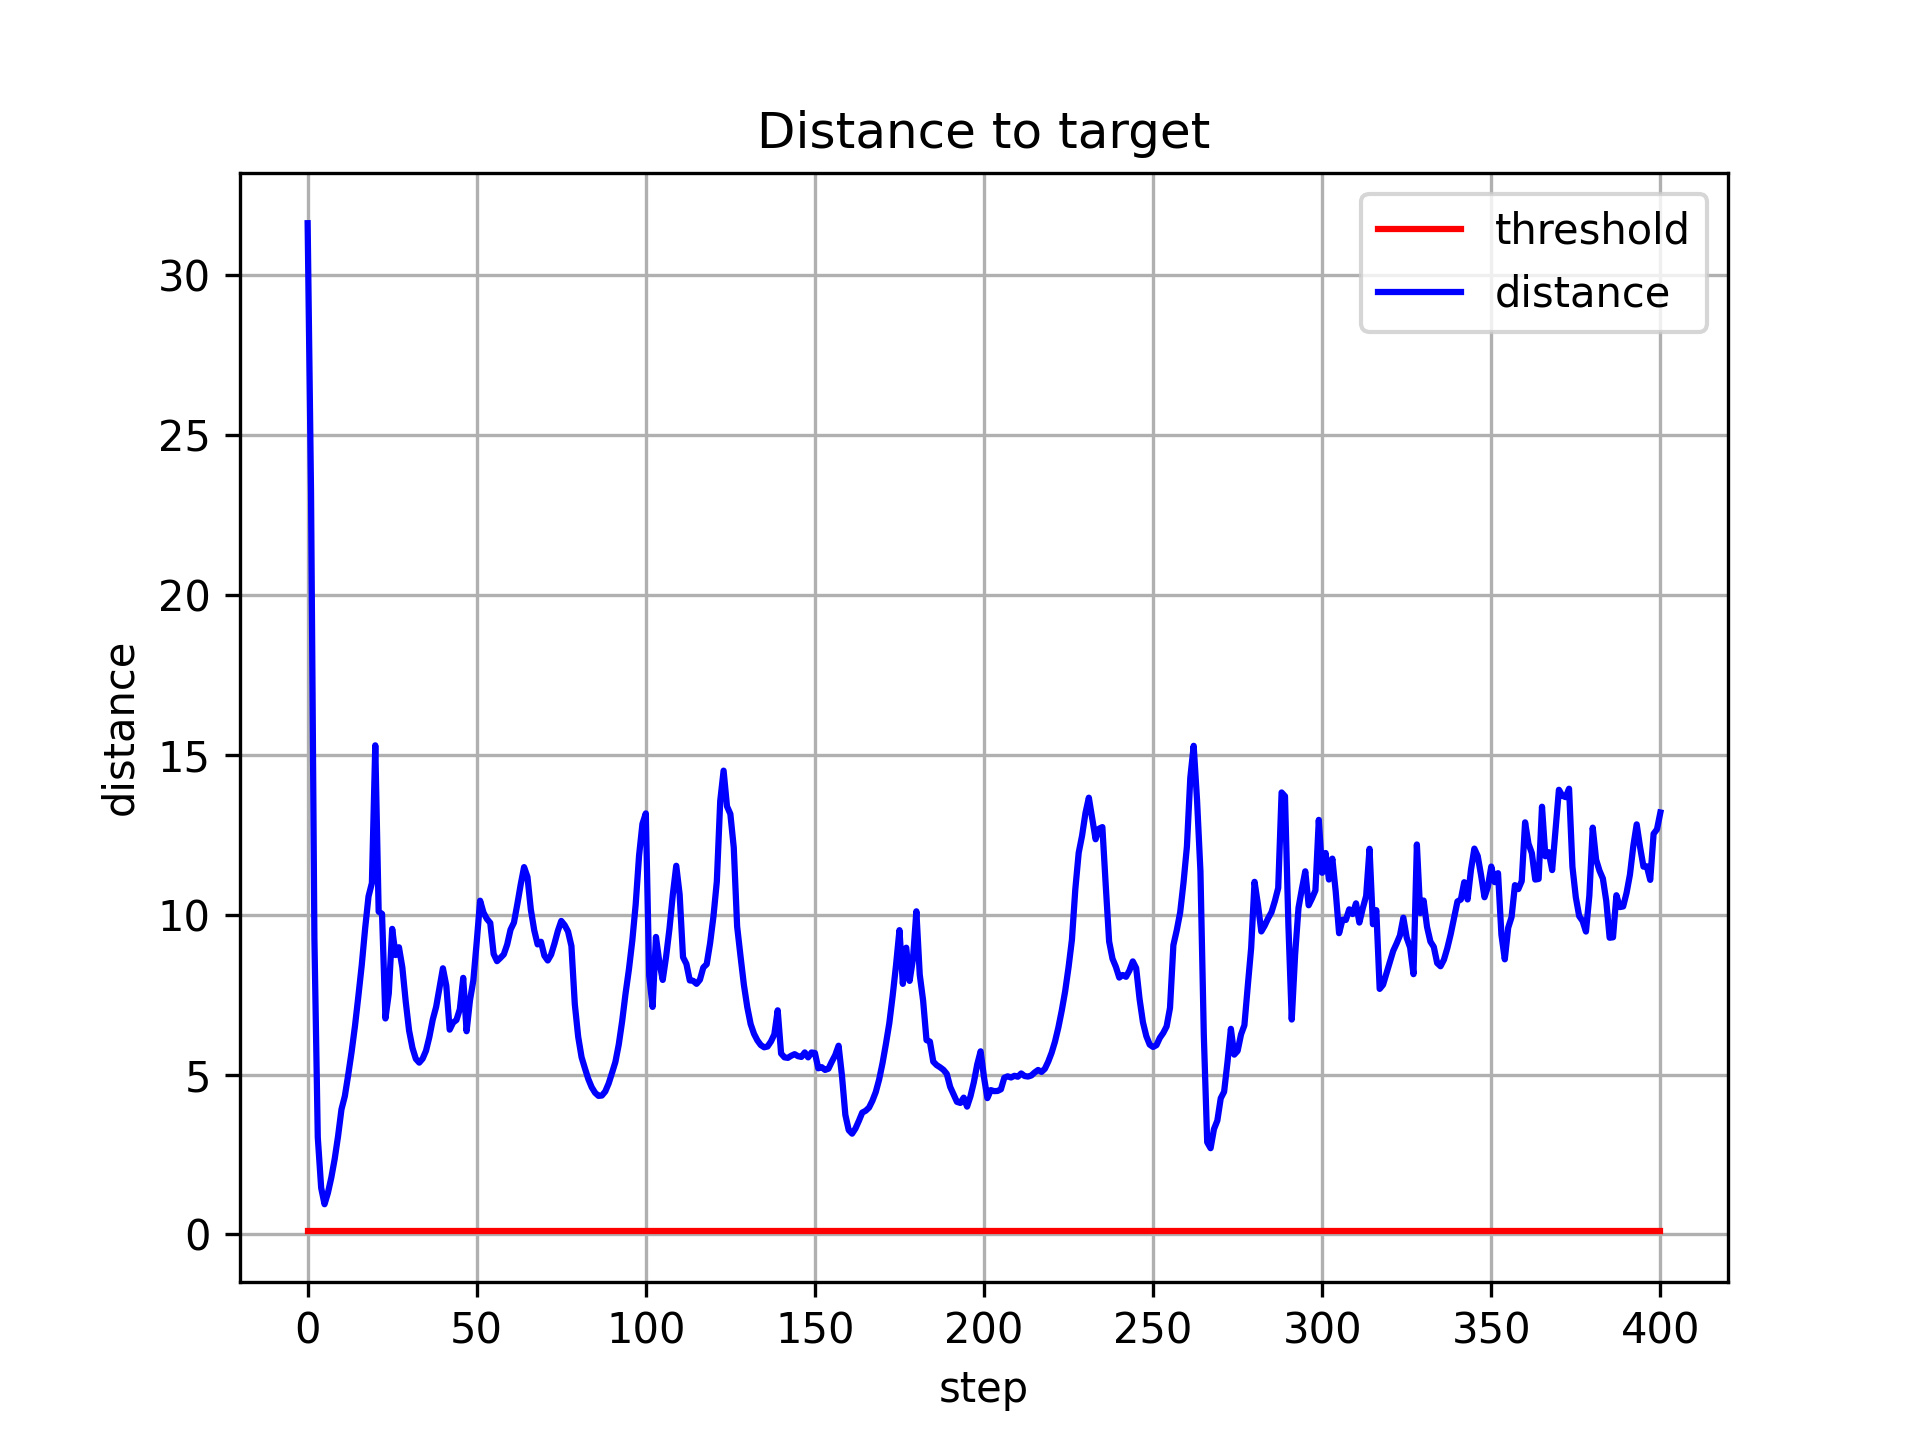
\includegraphics[width=0.31 \linewidth]{figures/experiments/Distance_to_target_baseline_20_1691619159_5000.png}
            \label{fig:SAC_baseline_inference/distance_20}
            }
    \end{center}
    \caption[SAC baseline inference]{Distance to target for each action outcome. The target is consistent at $[-0.5, 0.5] \cdot N$. The threshold of 0.1 at which an episode is concluded successfully is drawn in red.} 
    \label{fig:SAC_baseline_inference_distance}
\end{figure}
Another interesting detail to observe is the strategy an agent is following to reach the target position. Instead of moving almost in a straight line towards the target position the agent is moving its end-effector closely to the outer limit of its reach and then is descending towards the target. \todo{discussion}As we have seen in section \secref{sec:vanilla_sampling} randomly having an end-effector position far away from the origin is less probable compared to a position close to the origin. 

\subsection{Soft Actor-Critic + Variational Autoencoder}

In this section we are going to talk about the experimental results of combining the decoder from a Variational Autoencoder with soft actor critic. As we know from \chapref{chap:Methodology} we only use the decoder of the trained Variational Autoencoder with input from the corresponding state and a latent action directly sampled from the parameterized distribution from the actor network.

\begin{table}
    \begin{center}
        \begin{tabular}{ l | c  c | c  c | c  c}
        \textbf{$N$} & \multicolumn{6}{c}{latent dimension} \\
        \hline
        & \multicolumn{2}{c |}{2} & \multicolumn{2}{c |}{4} & \multicolumn{2}{c}{8} \\
        & random seed & epoch & random seed & epoch & random seed & epoch \\
        \hline
        2   & 1693105015  & 4950 & 1692461245   & 4890 & 1691608881   & 1480 \\
        5   & 1693096269  & 4495 & 1692476369   & 4795 & 1691606505   & 1290 \\
        10  & 1693098415  & 3615 & 1691627455   & 2535 & 1691608513   & 2485  \\
        15  & 1693103204  & 4815 & 1691628295   & 3845 & 1691618374   & 4760  \\
        \end{tabular}
    \end{center}
    \caption[Used VAE checkpoints for SAC]{Used checkpoints to train SAC with decoder from VAE. All experiments can be found in \texttt{results/vae/<$N$>\textunderscore<latent dimension>\textunderscore <random seed>/VAE\textunderscore<epoch>*.pt}}
    \label{tab:VAE_checkpoints_SAC}
\end{table}

As we have seen in the previous section we carried out VAE experiments with three different latent space dimensions. Accordingly we trained ten SAC runs for each latent space size and number of joints with $N \in [2, 5, 10, 15]$. We used the best VAE checkpoint available according to the overall validation loss. The detailed listing which checkpoints where actually used can be found in \tabref{tab:VAE_checkpoints_SAC}. 

\begin{figure}
    \begin{center}
        \subfloat[mean episode reward per step averaged over the last 20 episodes. With a \textbf{latent dimension = 2}]{
            
\includegraphics[width=0.31 \linewidth]{figures/place_holder.png}
            \label{fig:SAC_latent_4/reward}
            }
        \hfill
        \subfloat[mean episode reward per step averaged over the last 20 episodes. With a \textbf{latent dimension = 4}]{
            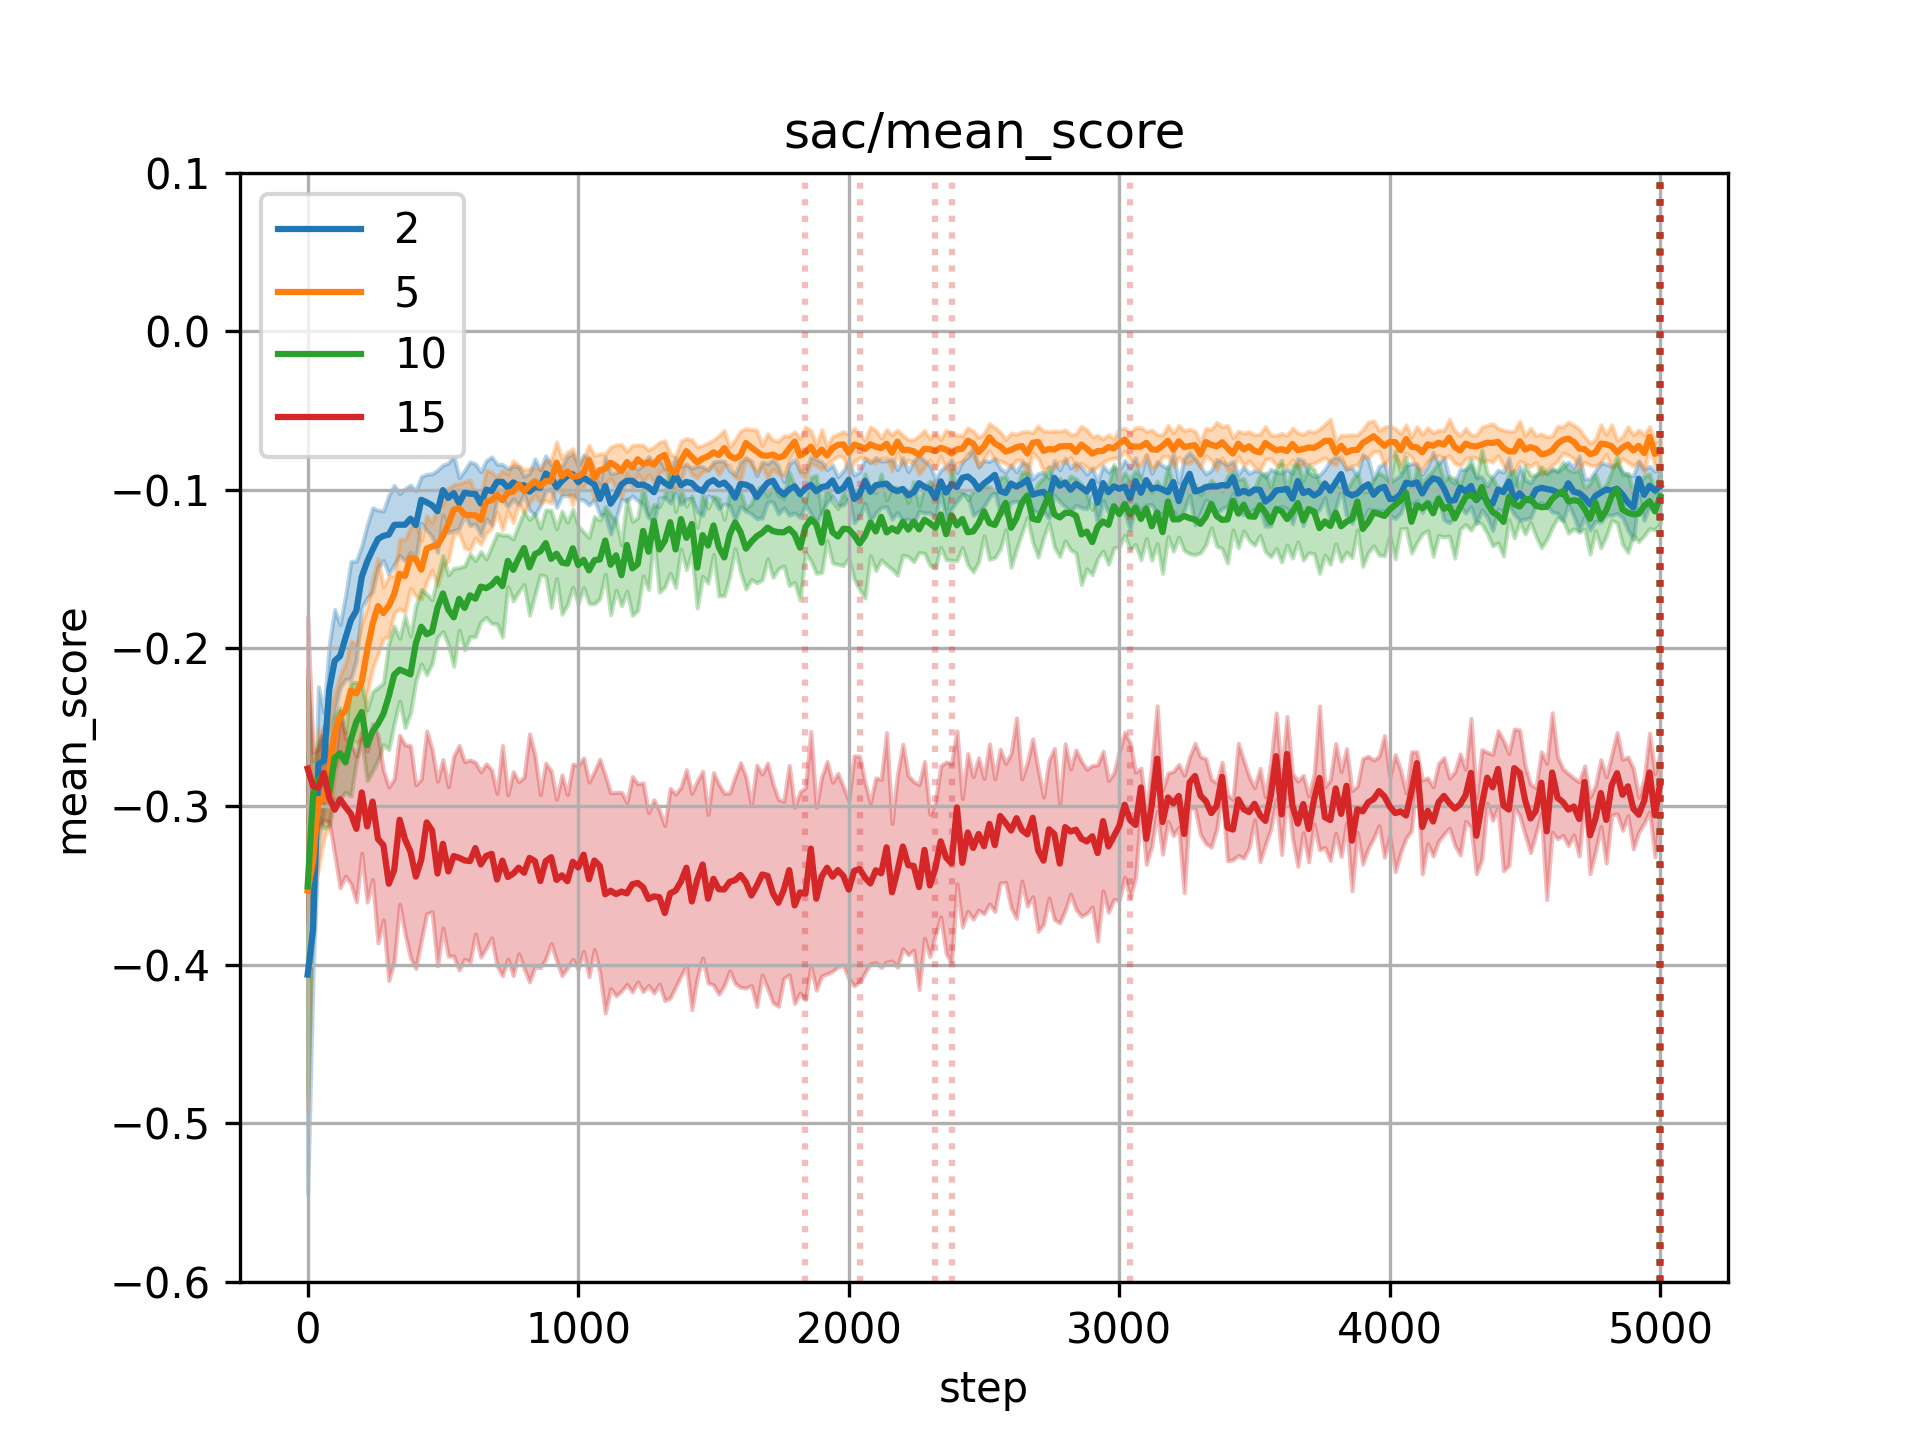
\includegraphics[width=0.31 \linewidth]{figures/experiments/sac_latent_actor_4_mean_score.png}
            \label{fig:SAC_latent_4/reward}
            }
        \hfill
        \subfloat[mean episode reward per step averaged over the last 20 episodes. With a \textbf{latent dimension = 8}]{
            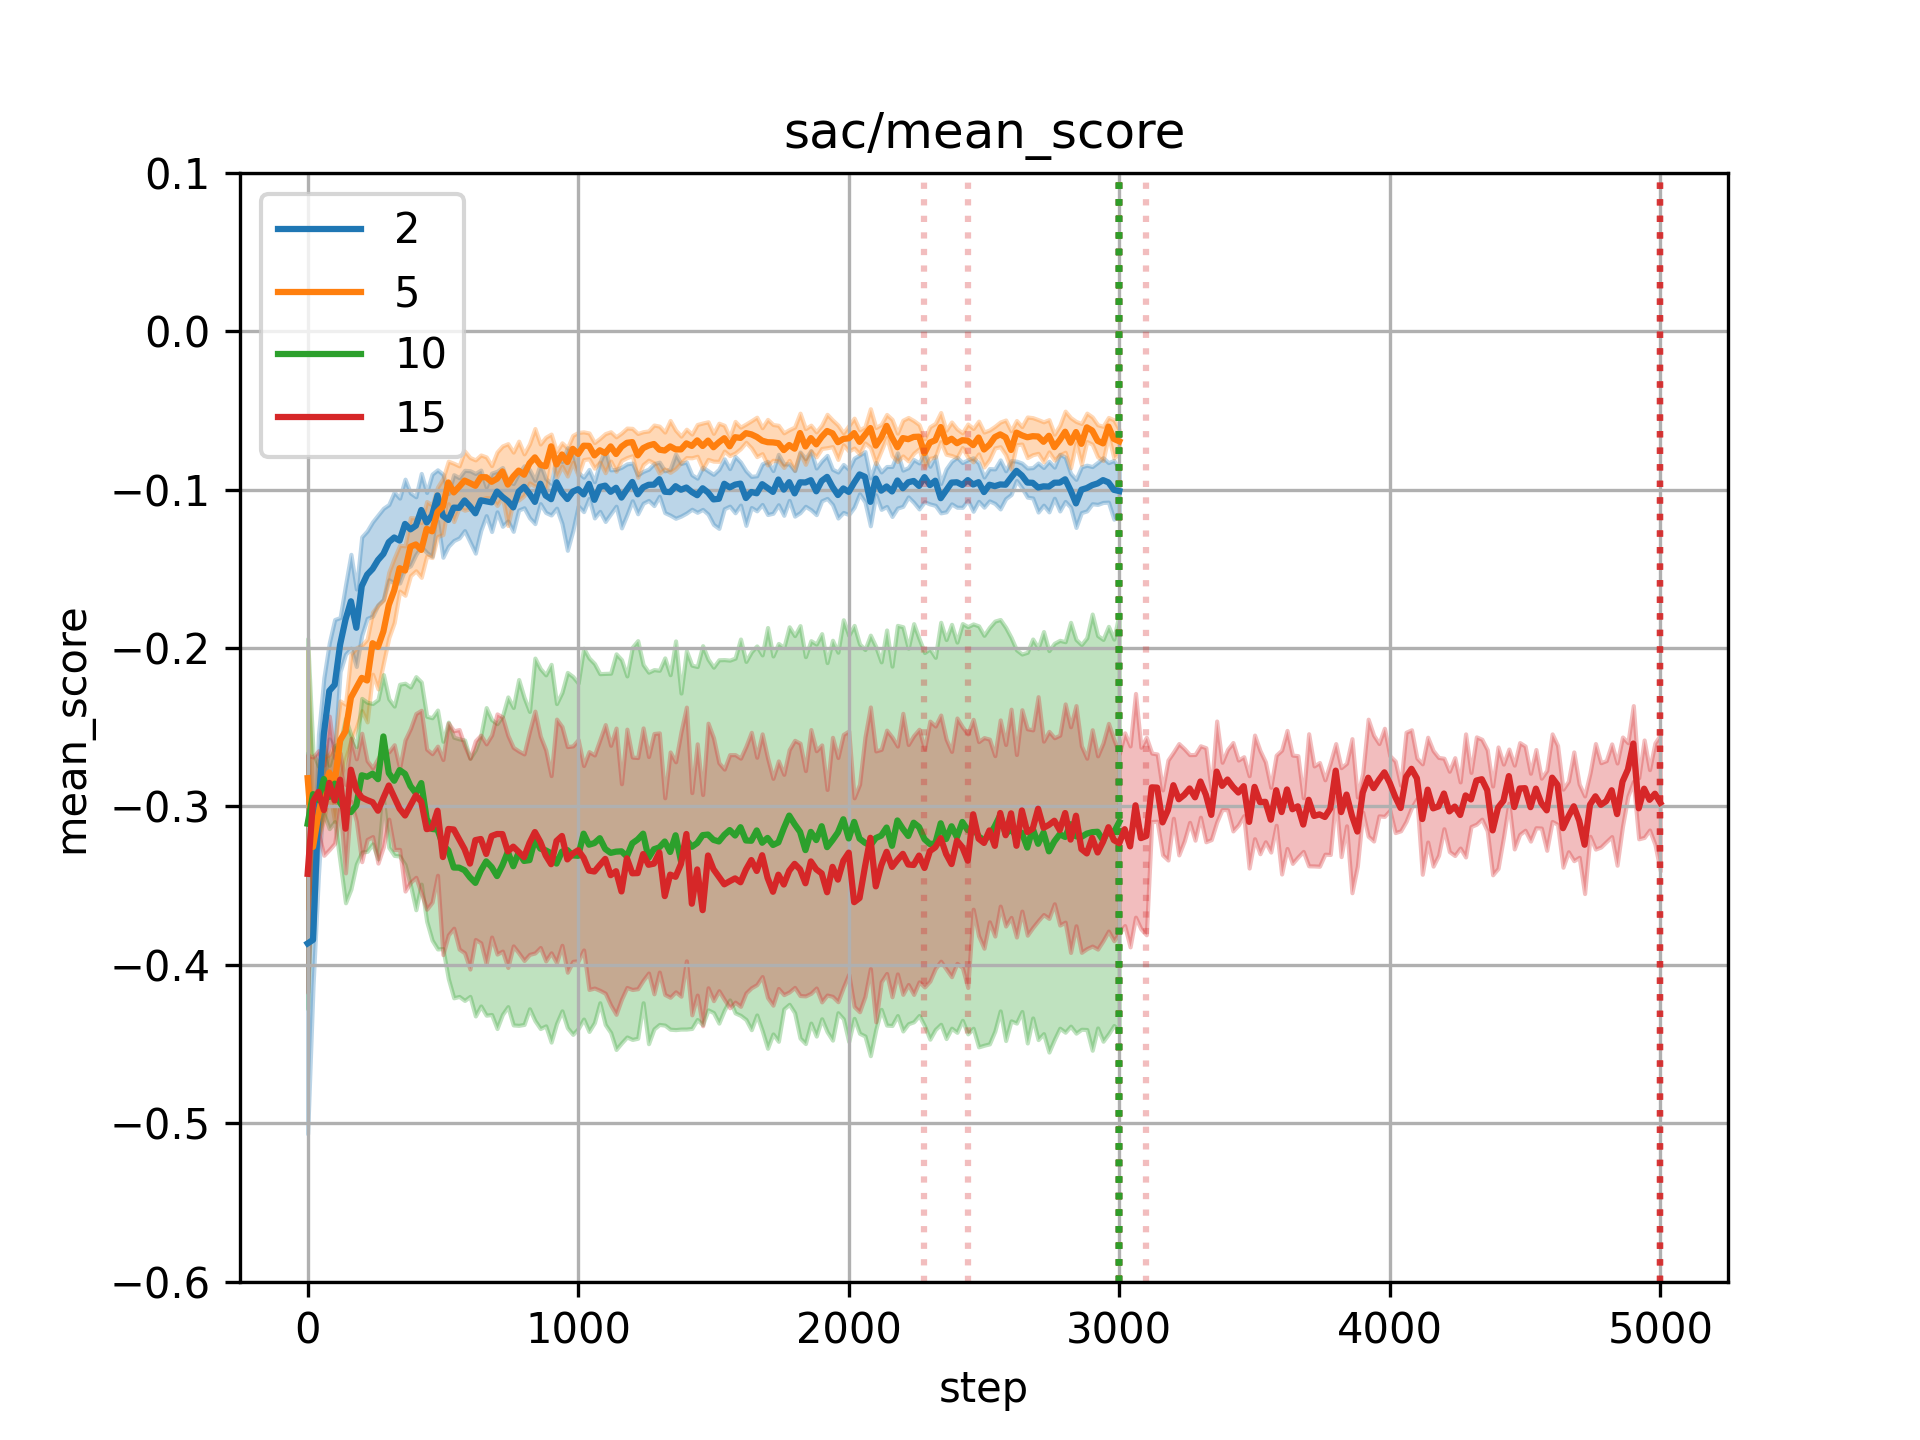
\includegraphics[width=0.31 \linewidth]{figures/experiments/sac_latent_actor_8_mean_score.png}
            \label{fig:SAC_latent_8/reward}
            }
        \\
        \subfloat[mean episode length avergaed over the last 20 episodes. With a \textbf{latent dimension = 2}]{
            
\includegraphics[width=0.31 \linewidth]{figures/place_holder.png}
            \label{fig:SAC_latent_4/episode_len}
            }
        \hfill
        \subfloat[mean episode length avergaed over the last 20 episodes. With a \textbf{latent dimension = 4}]{
        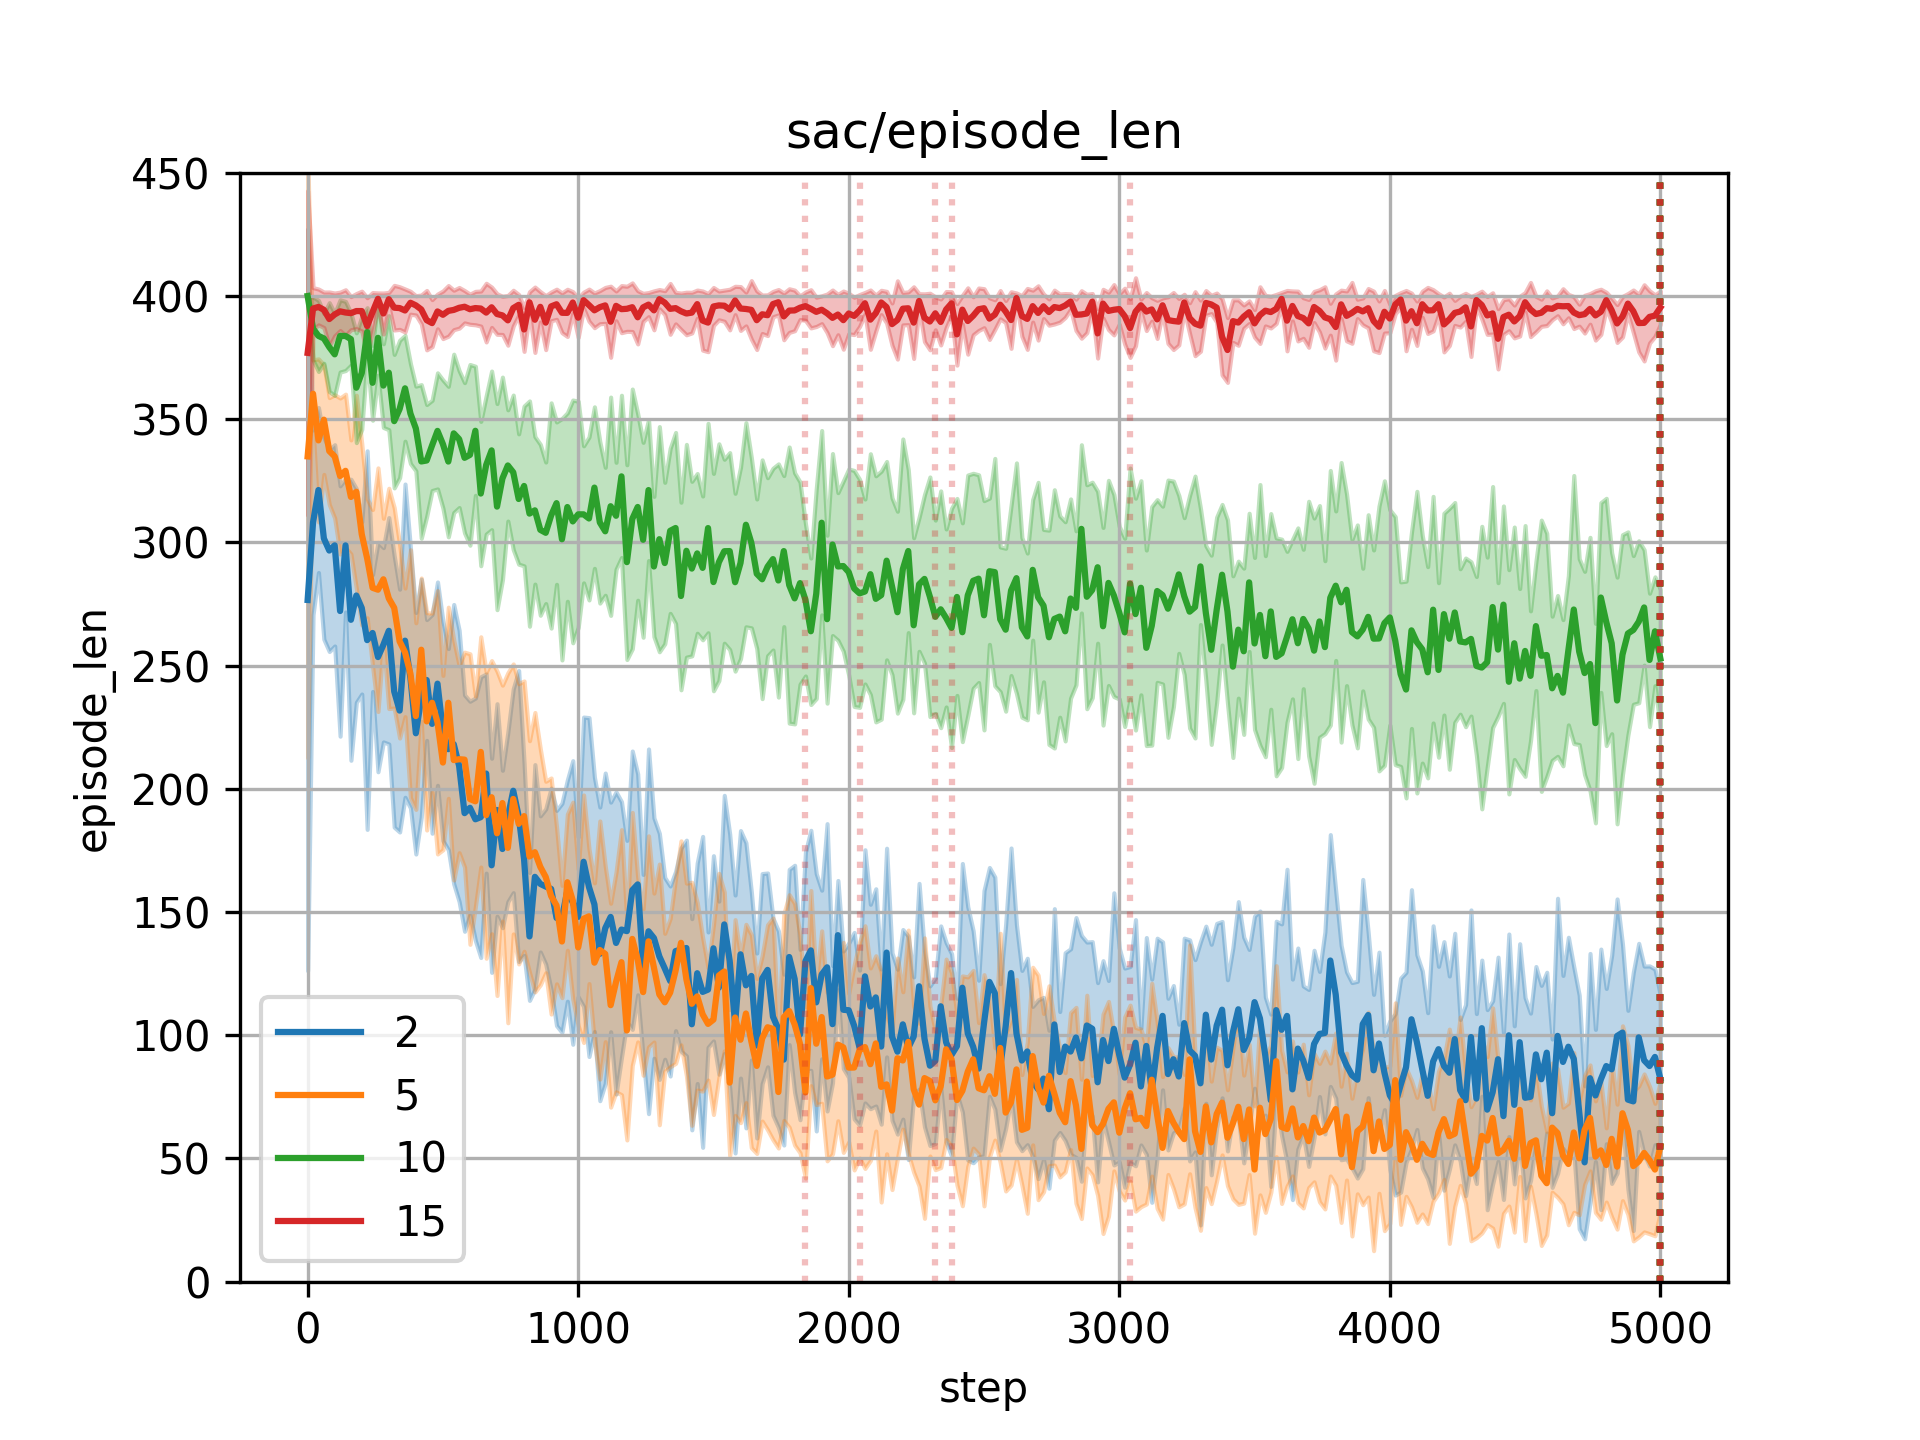
\includegraphics[width=0.31 \linewidth]{figures/experiments/sac_latent_actor_4_episode_len.png}
            \label{fig:SAC_latent_4/episode_len}
            }
        \hfill
        \subfloat[mean episode length avergaed over the last 20 episodes. With a \textbf{latent dimension = 8}]{
        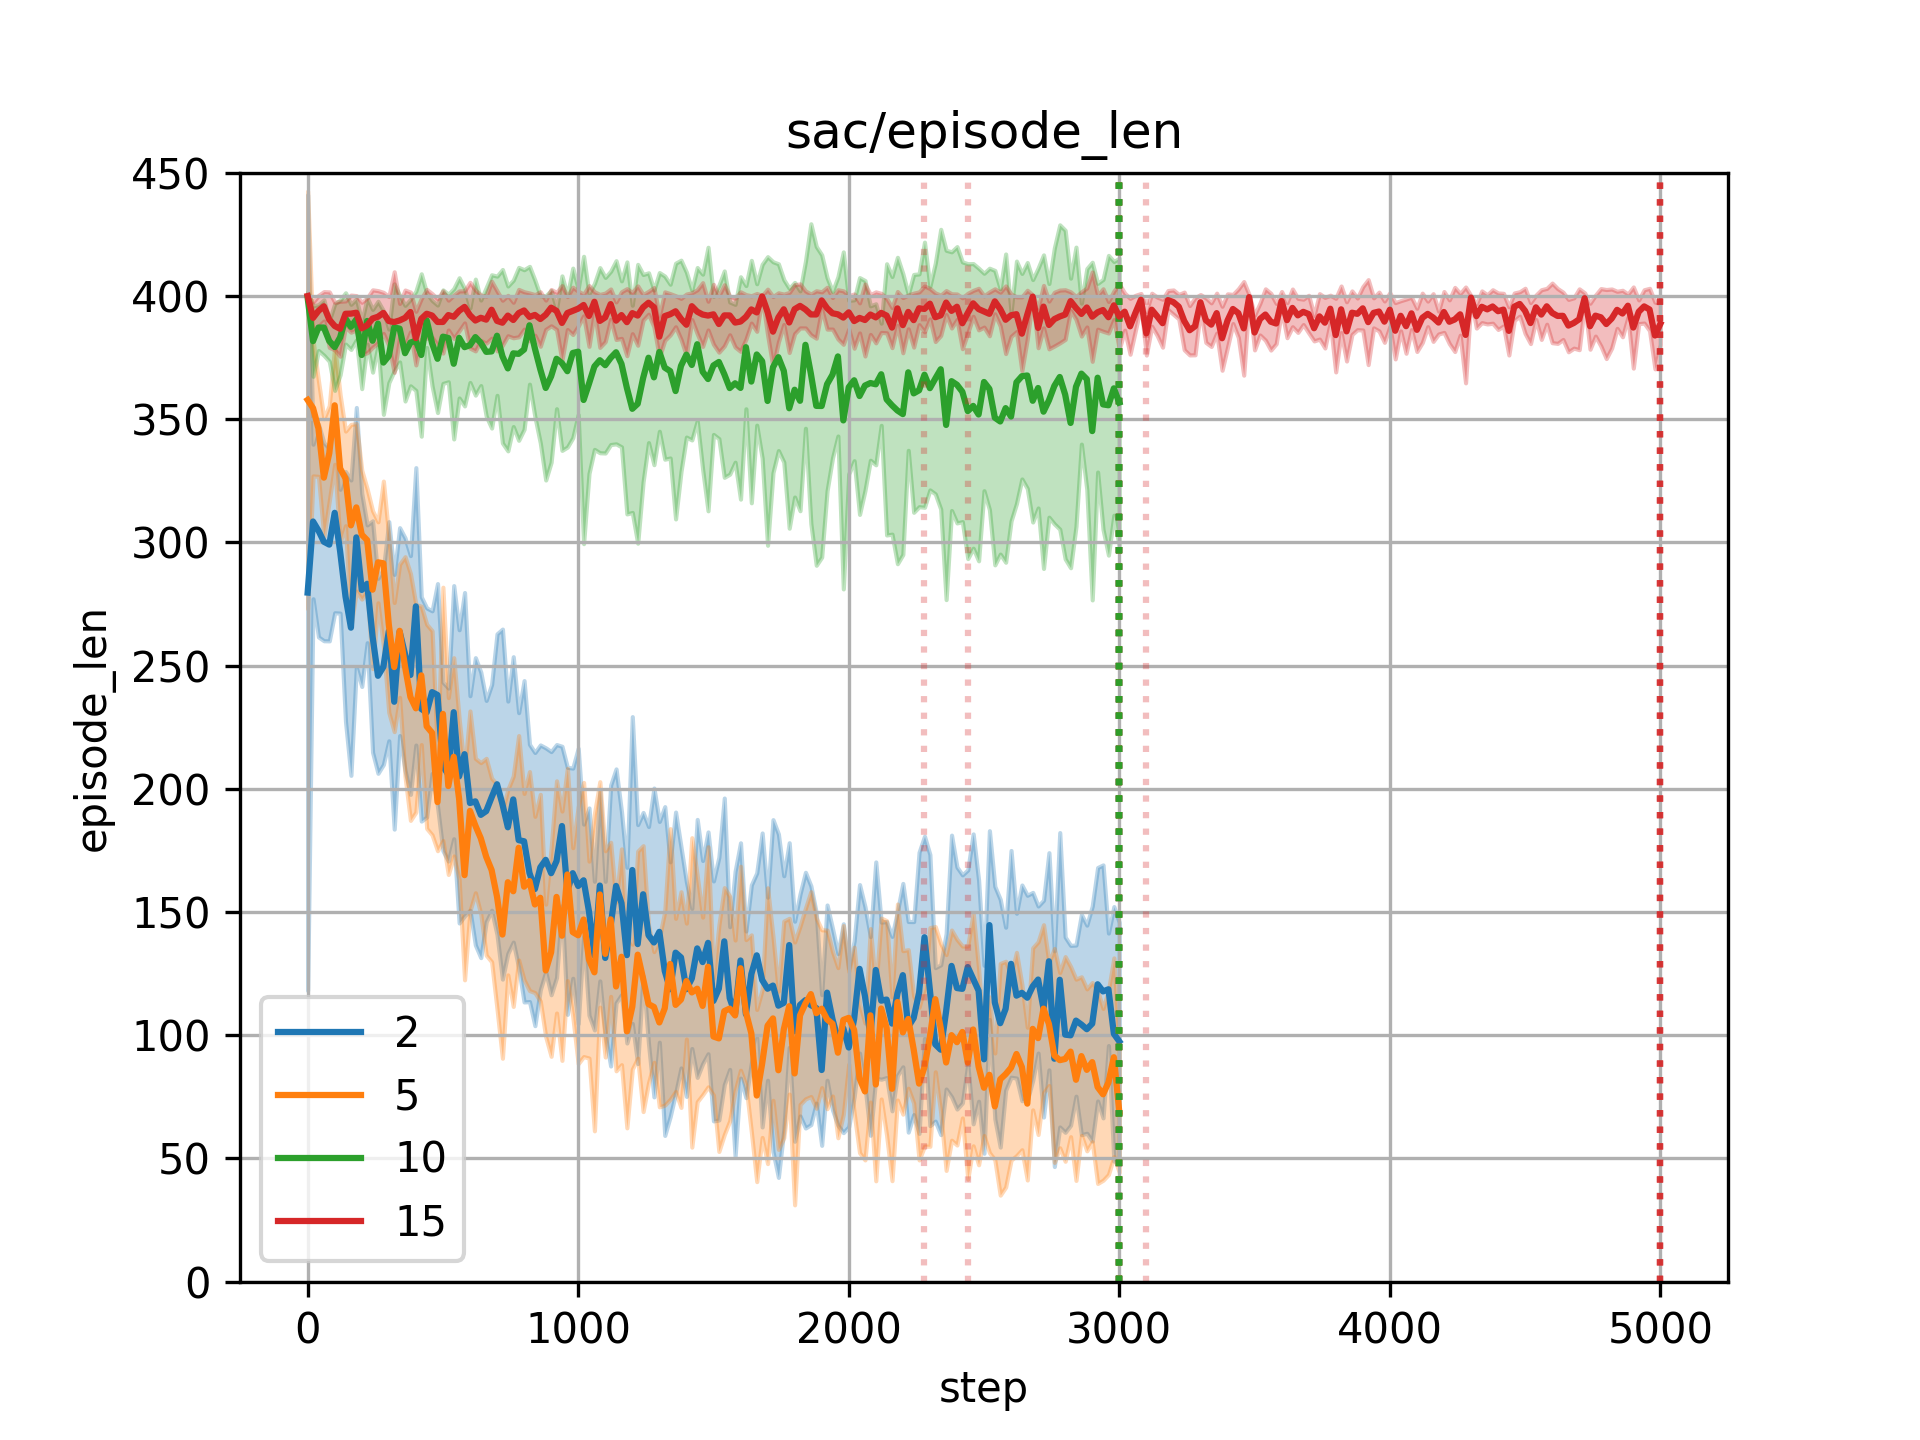
\includegraphics[width=0.31 \linewidth]{figures/experiments/sac_latent_actor_8_episode_len.png}
            \label{fig:SAC_latent_8/episode_len}
            }
    \end{center}
    \caption[SAC + VAE on latent dim = 4]{SAC + decoder form VAE with different latent dimensions. Each experiment was conducted 10 times with different random seeds. The solid strong line is the mean over those 10 experiments. The color shaded area covering the mean is the standard deviation around the mean.}
    \label{fig:SAC_latent_4}
\end{figure}

\begin{figure}
    \begin{center}
        \subfloat[$N = 2$]{
            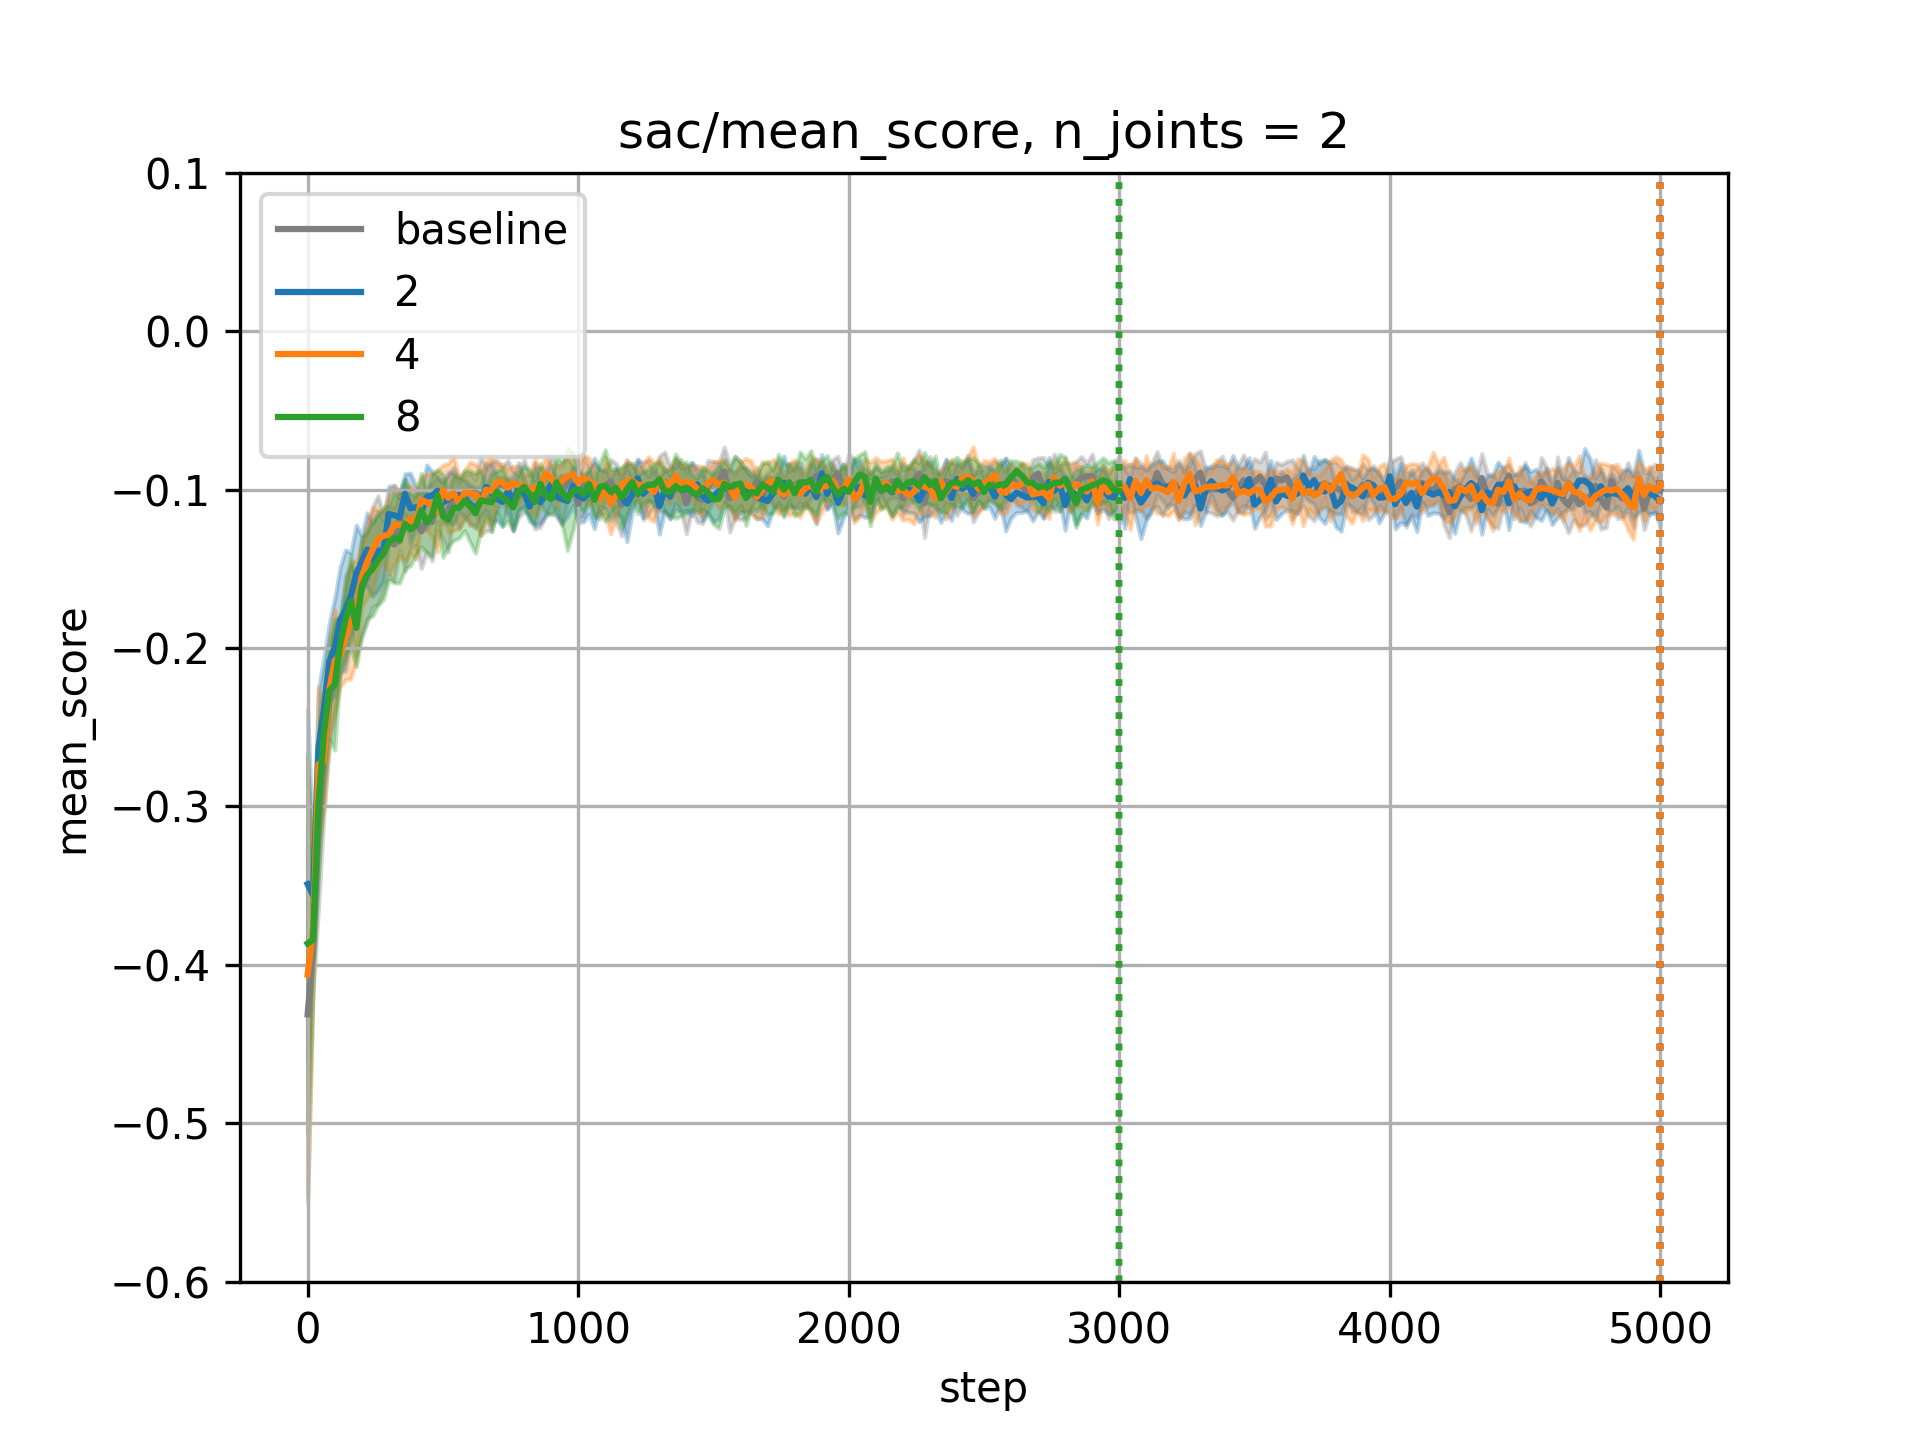
\includegraphics[width=0.23 \linewidth]{figures/experiments/sac_latent_comp_2_vae_mean_score.png}
            \label{fig:SAC_latent_comparison_mean_score/2}
            }
        \hfill
        \subfloat[$N = 5$]{
        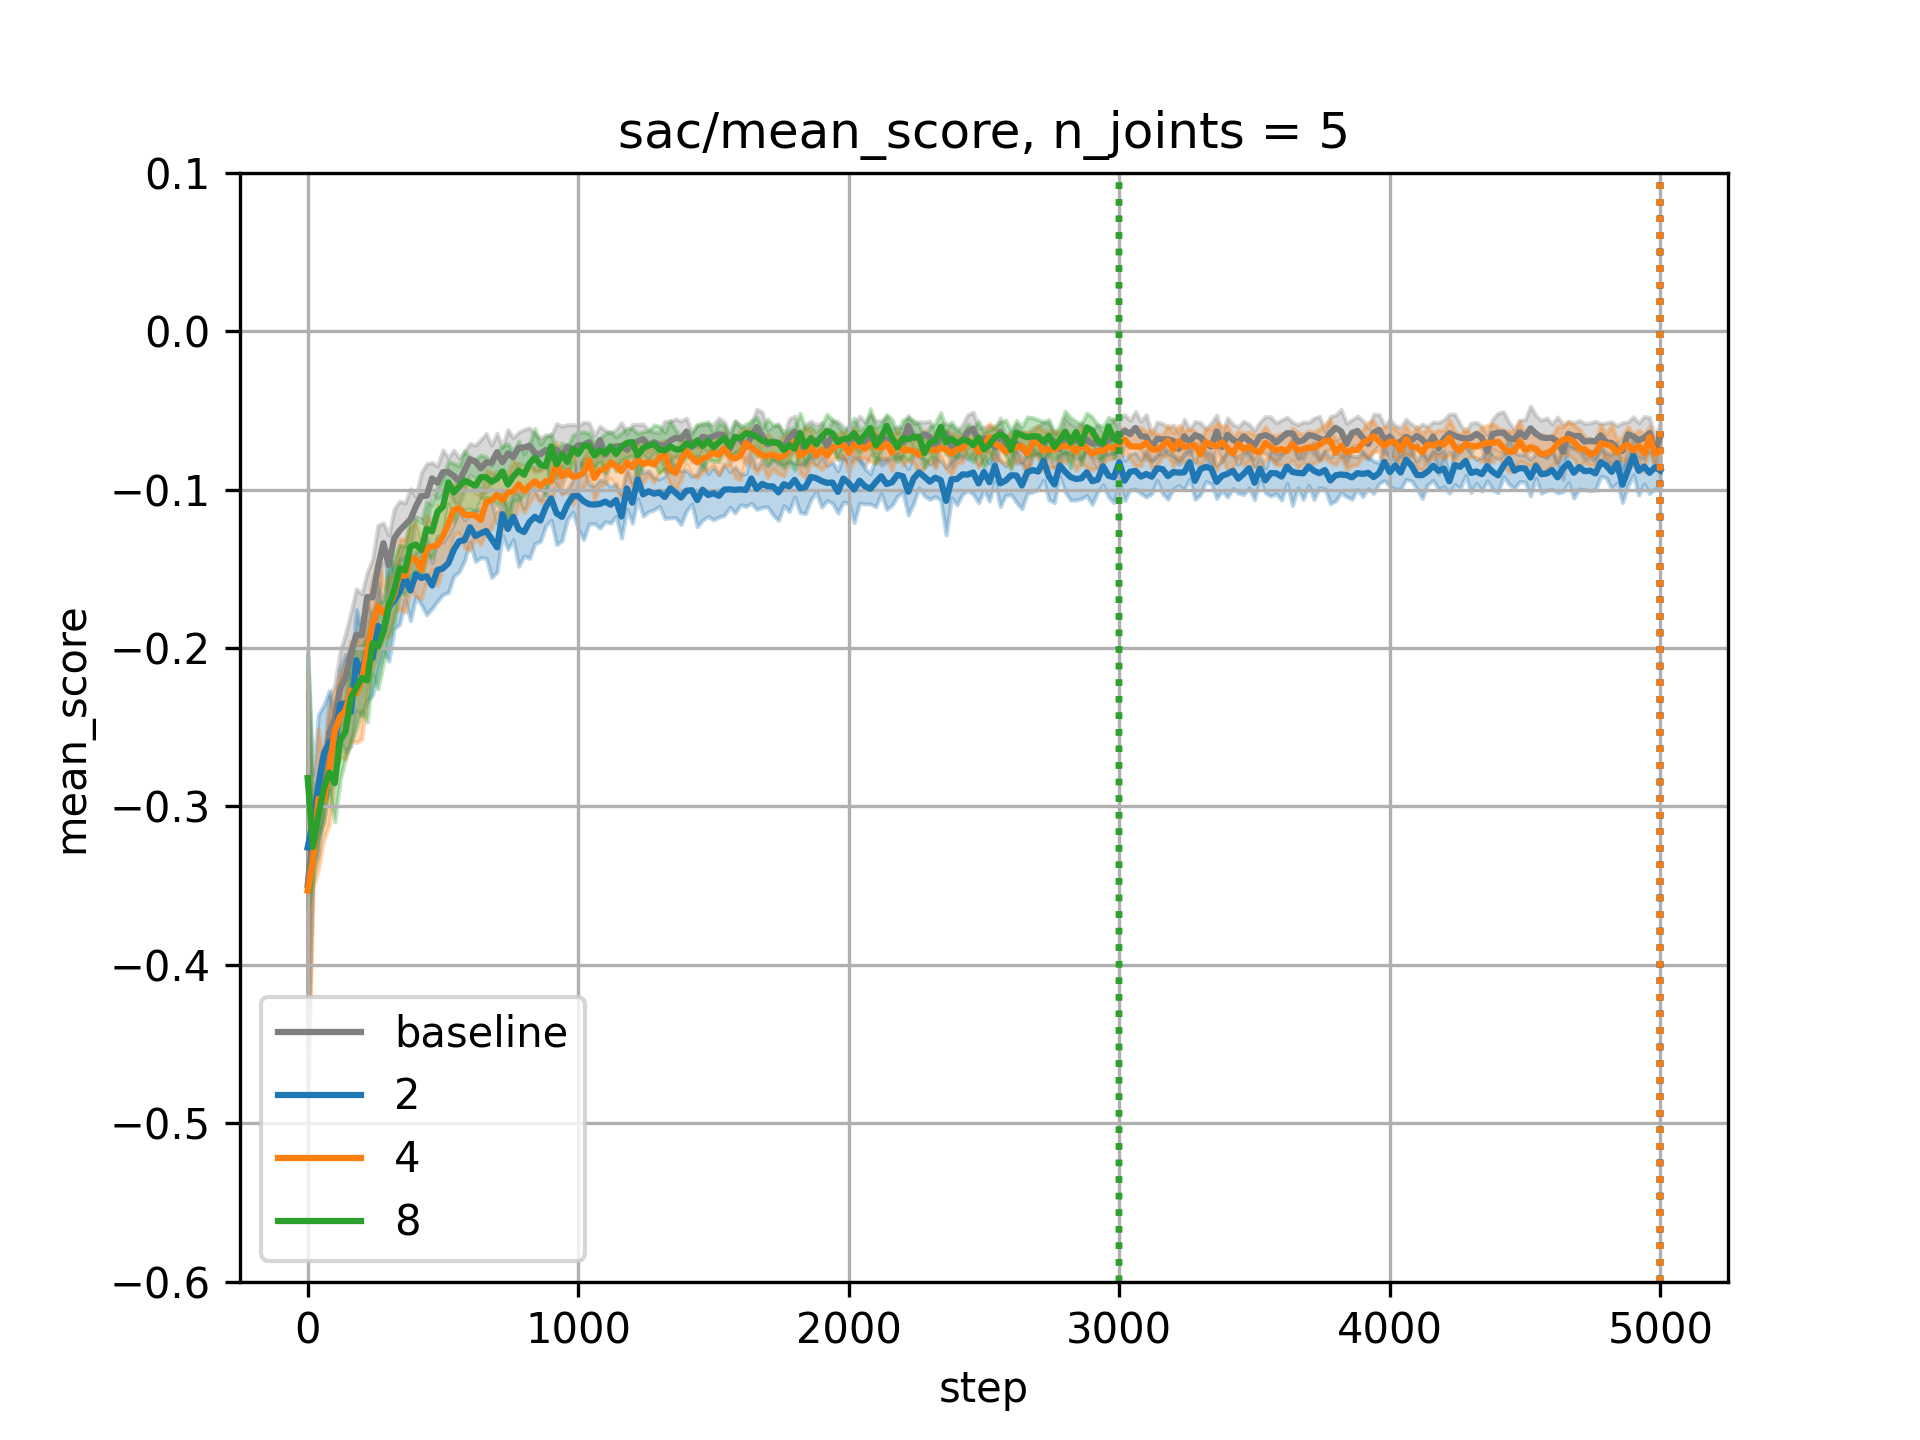
\includegraphics[width=0.23 \linewidth]{figures/experiments/sac_latent_comp_5_vae_mean_score.png}
            \label{fig:SAC_latent_comparison_mean_score/5}
            }
        \hfill    
        \subfloat[$N = 10$]{
            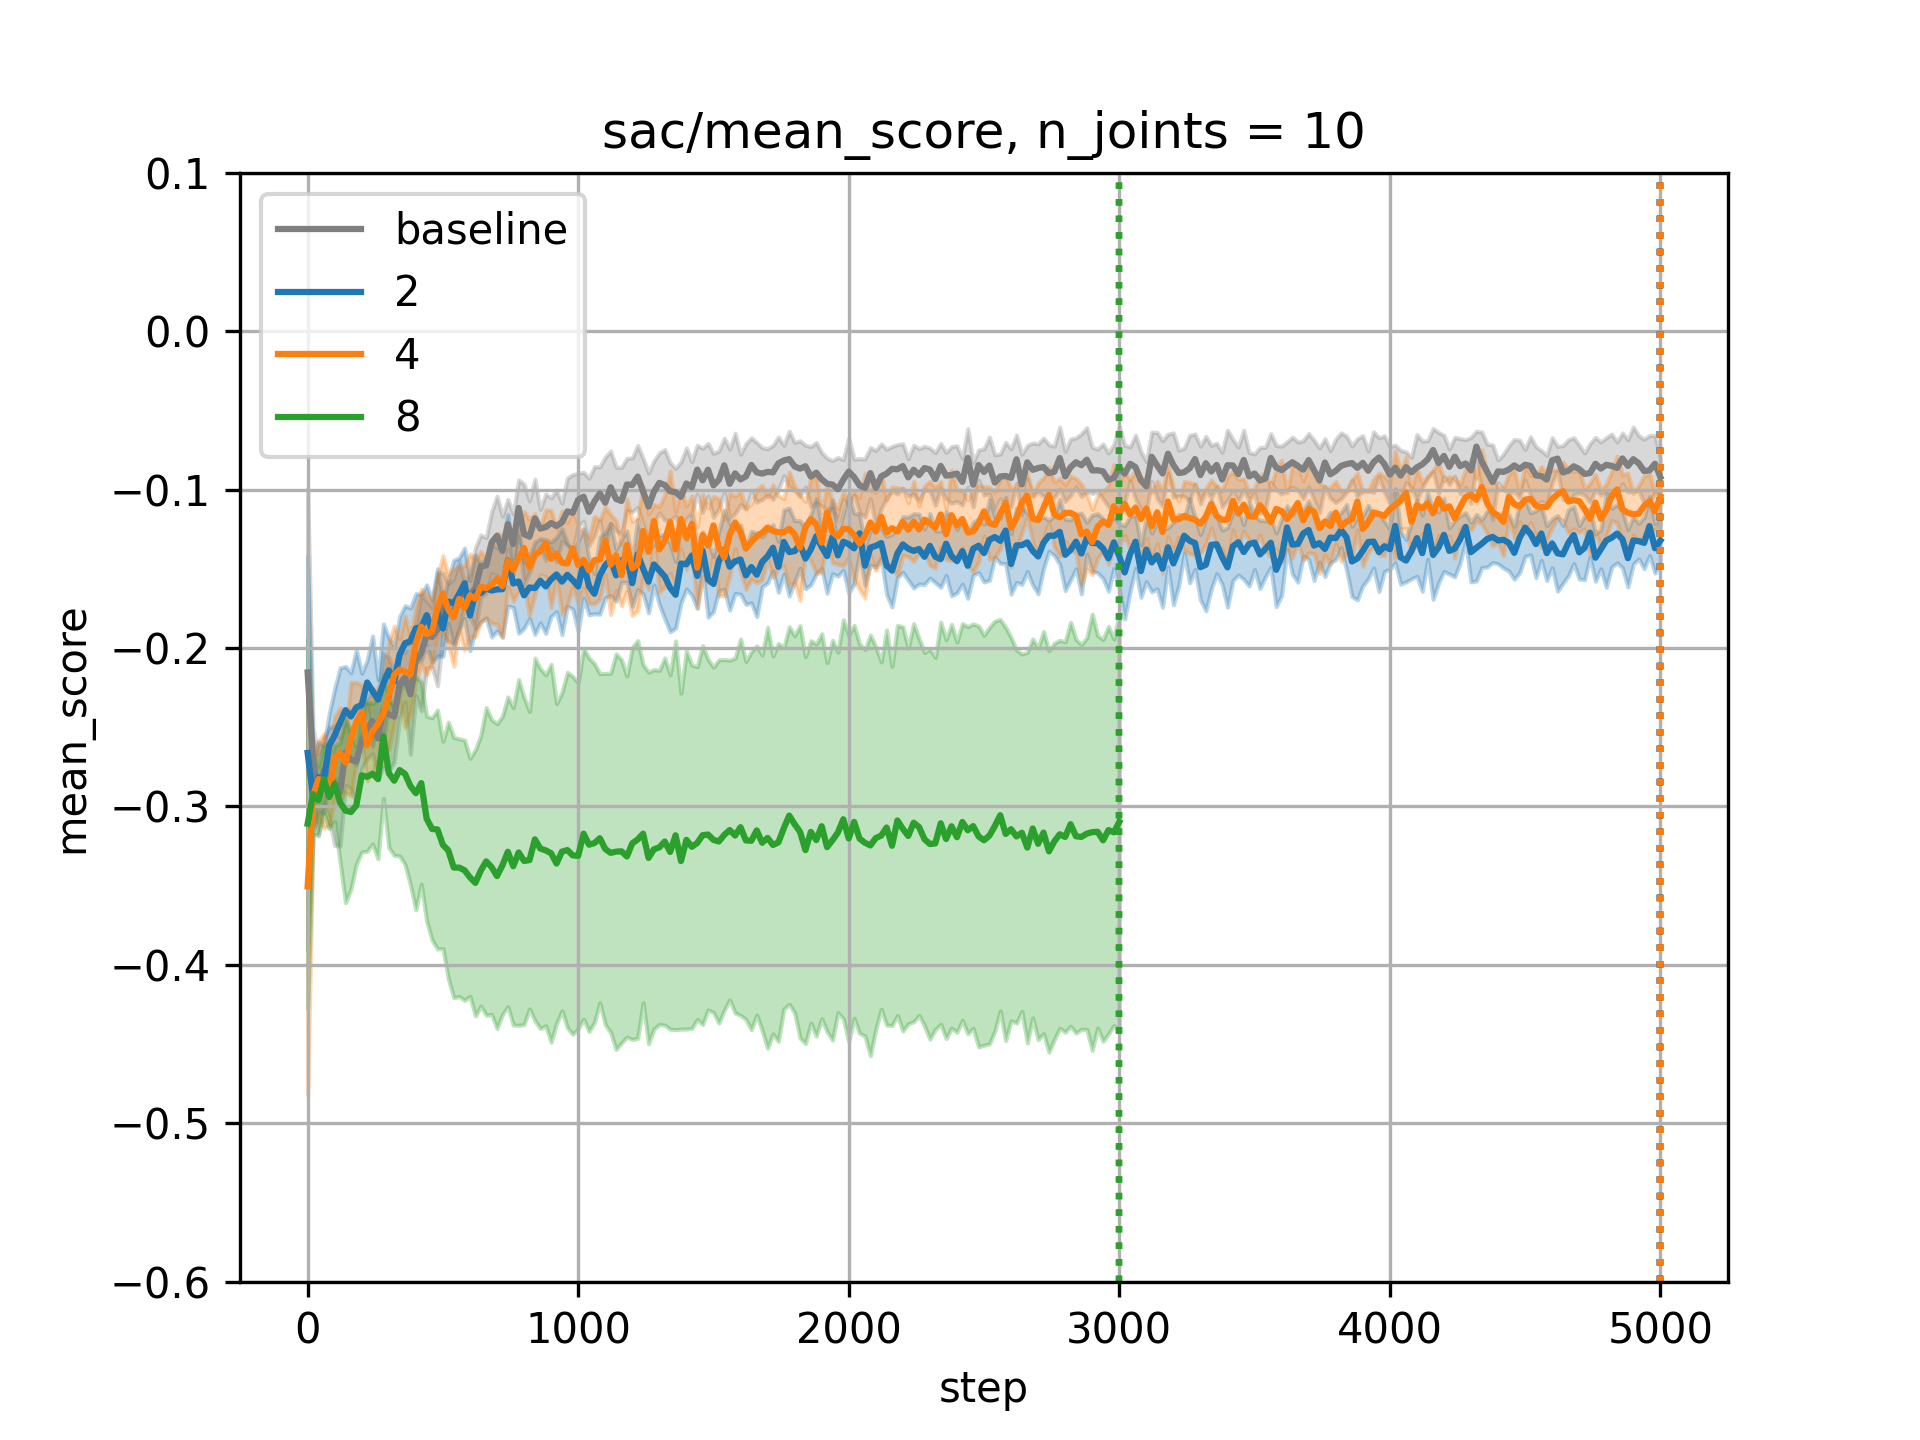
\includegraphics[width=0.23 \linewidth]{figures/experiments/sac_latent_comp_10_vae_mean_score.png}
            \label{fig:SAC_latent_comparison_mean_score/10}
            }
        \hfill
        \subfloat[$N = 15$]{
        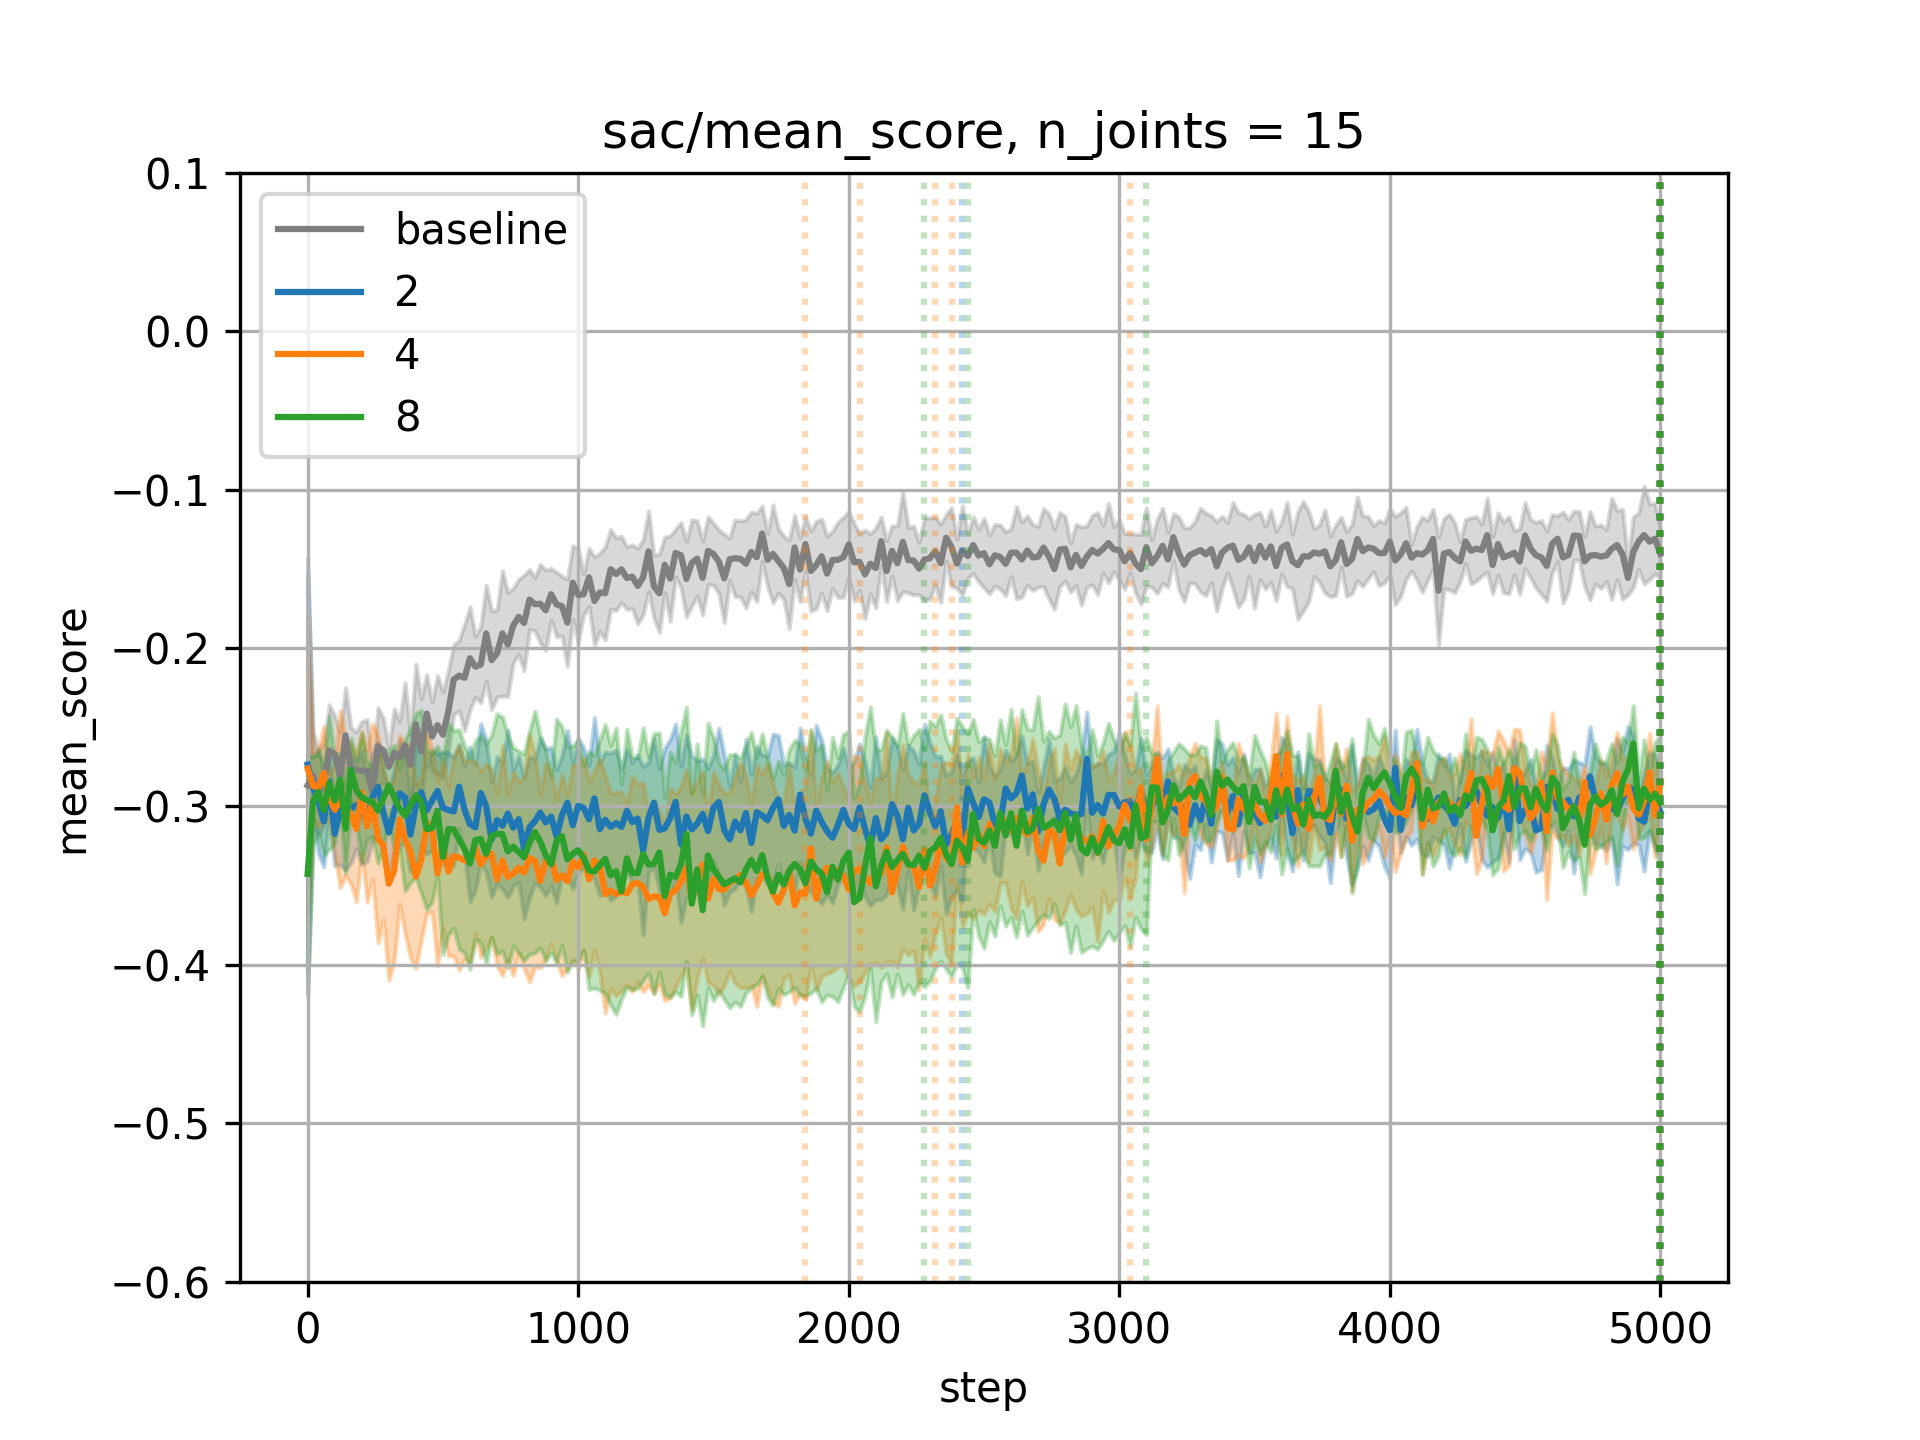
\includegraphics[width=0.23 \linewidth]{figures/experiments/sac_latent_comp_15_vae_mean_score.png}
            \label{fig:SAC_latent_comparison_mean_score/15}}
    \end{center}
    \caption[SAC + VAE latent dimension comparison]{Shown are the collected mean scores over the the last 20 episodes per step, compared different latent dimensions and the baseline. Solid line is the mean over 10 experiments and the color shaded area is the corresponding standard deviation. Higher means better with 0 as the maximum. The colored dotted lines mark an end of an experiment.}
    \label{fig:SAC_latent_comparison_mean_score}
\end{figure}

In \figref{fig:SAC_latent_comparison_mean_score} we can observe what difference the choice of latent dimension has on the performance of the Soft Actor Critic algorithm. Quite obviously to see is that the the choice of latent dimension really starts to matter after 5 joints. Where at 10 joints 2 and 4 succeed but 8 doesn't. This is clearly related to the performance of the VAE during its training. There we were also able to see that the latent dimension has an impact of the reconstruction loss performance of the VAE. Therefor it is no surprise to see that the best VAE checkpoints on 15 joints and the best VAE checkpoint on 10 joints with a latent dimension of 8 fails for the SAC + VAE setting. 

By having a closer look into the difference between the collected mean score we can see that for two joints all mean curves, the solid ones, are packet closely together where at five joints we can start to see a slight decrease in performance at 1000 epochs continuing up to 5000 epochs, between the experiments done with a latent dimension of two and the others.\\
This decrease is even more noticeable at ten joints where is now a gap between the experiments done with a latent dimension of four and the baseline experiments too. \todo{set in perspective of VAE performance}
\begin{figure}
    \begin{center}
        \subfloat[$N = 2$]{
            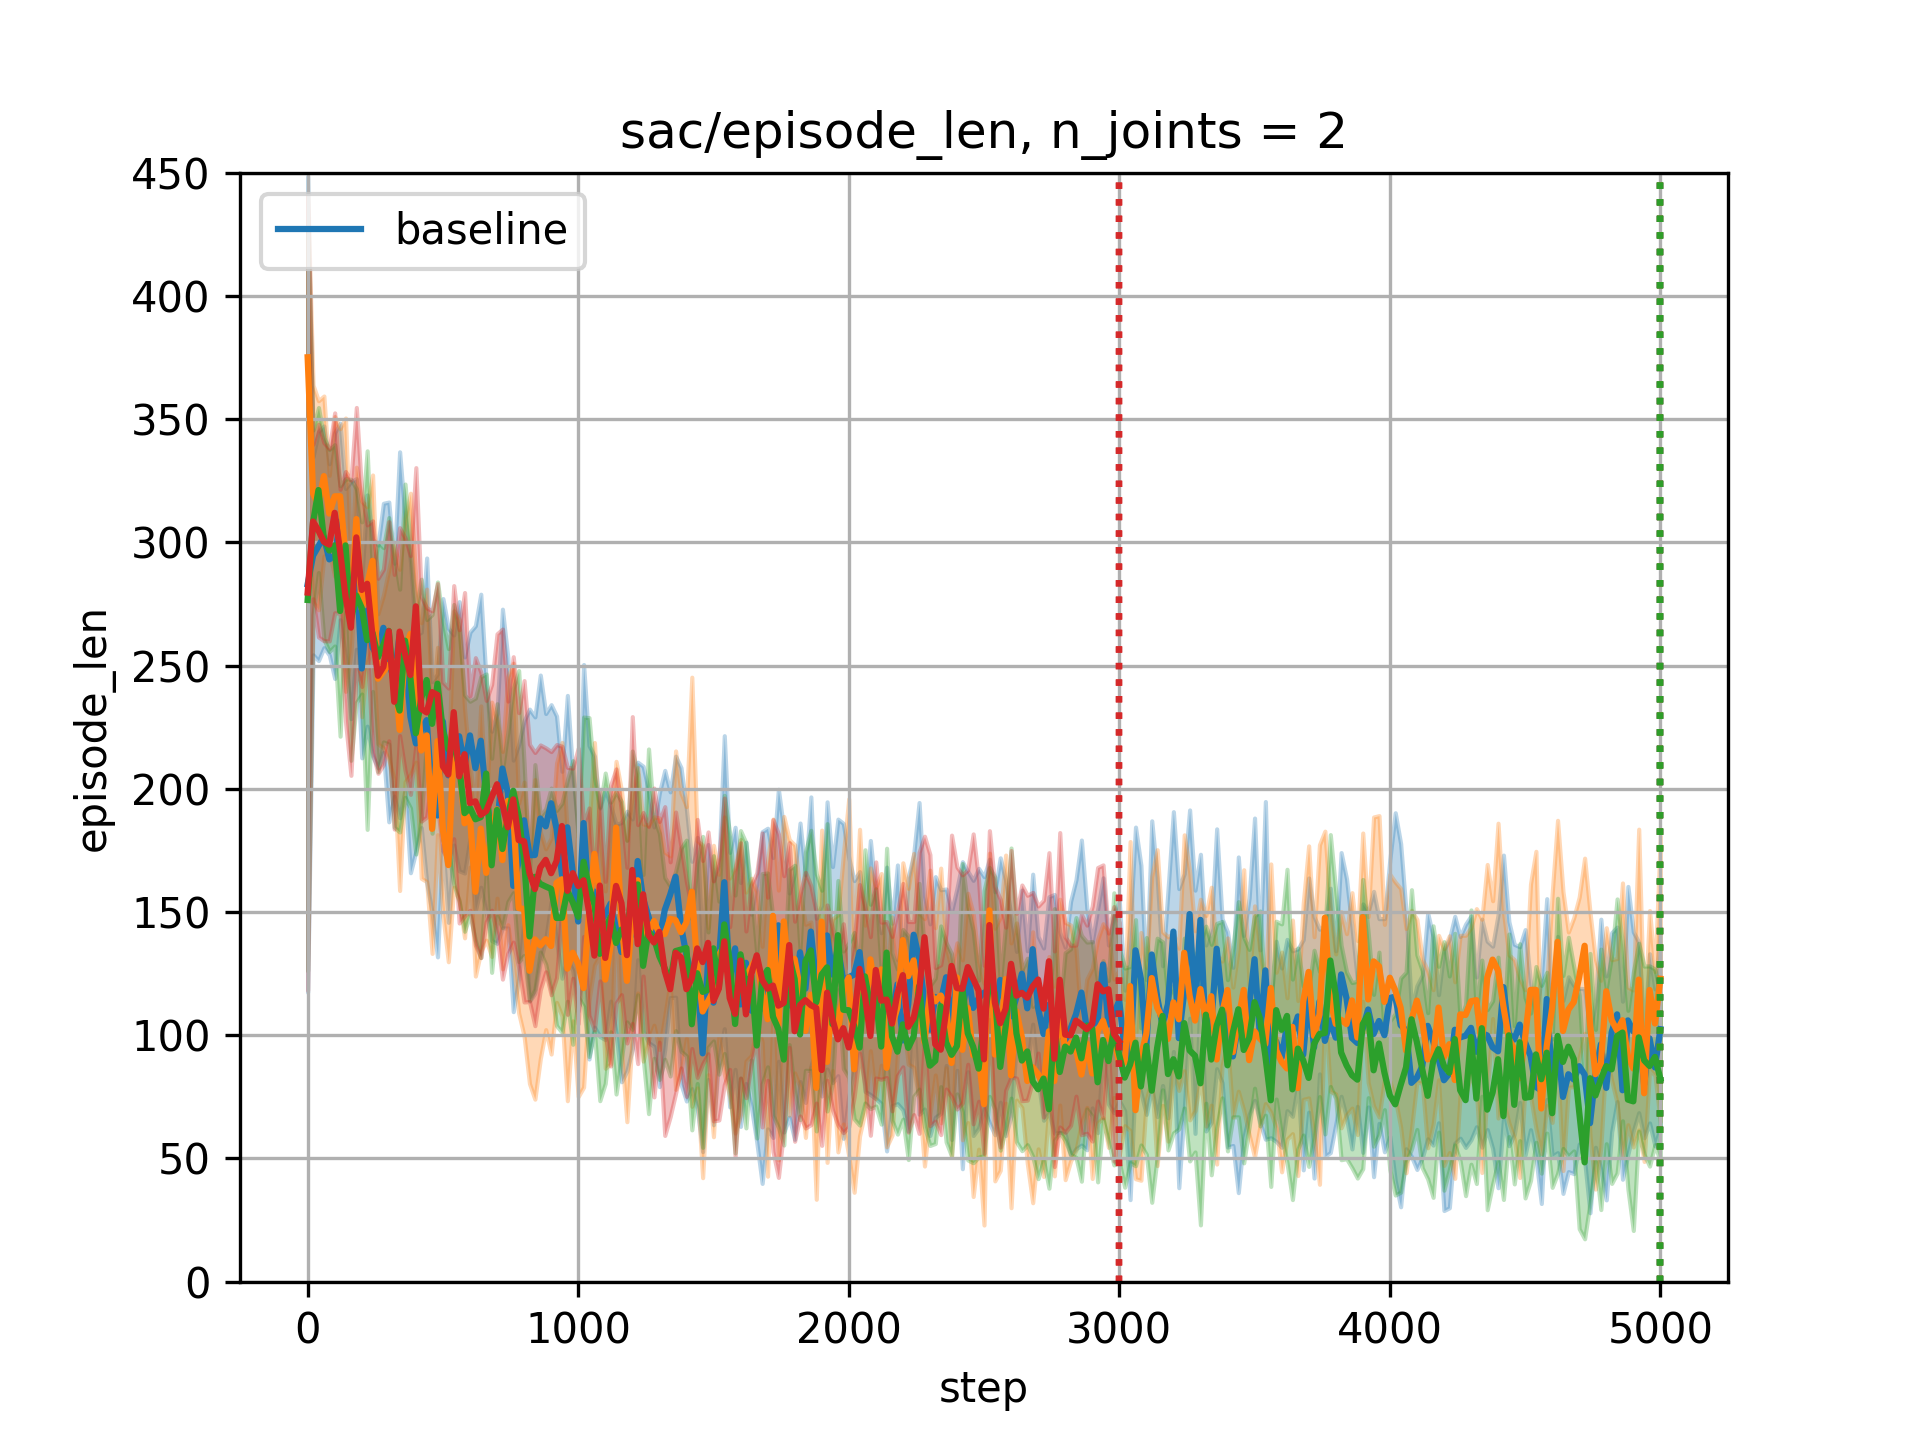
\includegraphics[width=0.23 \linewidth]{figures/experiments/sac_latent_comp_2_vae_episode_len.png}
            \label{fig:SAC_latent_comparison_episode_len/2}
            }
        \hfill
        \subfloat[$N = 5$]{
        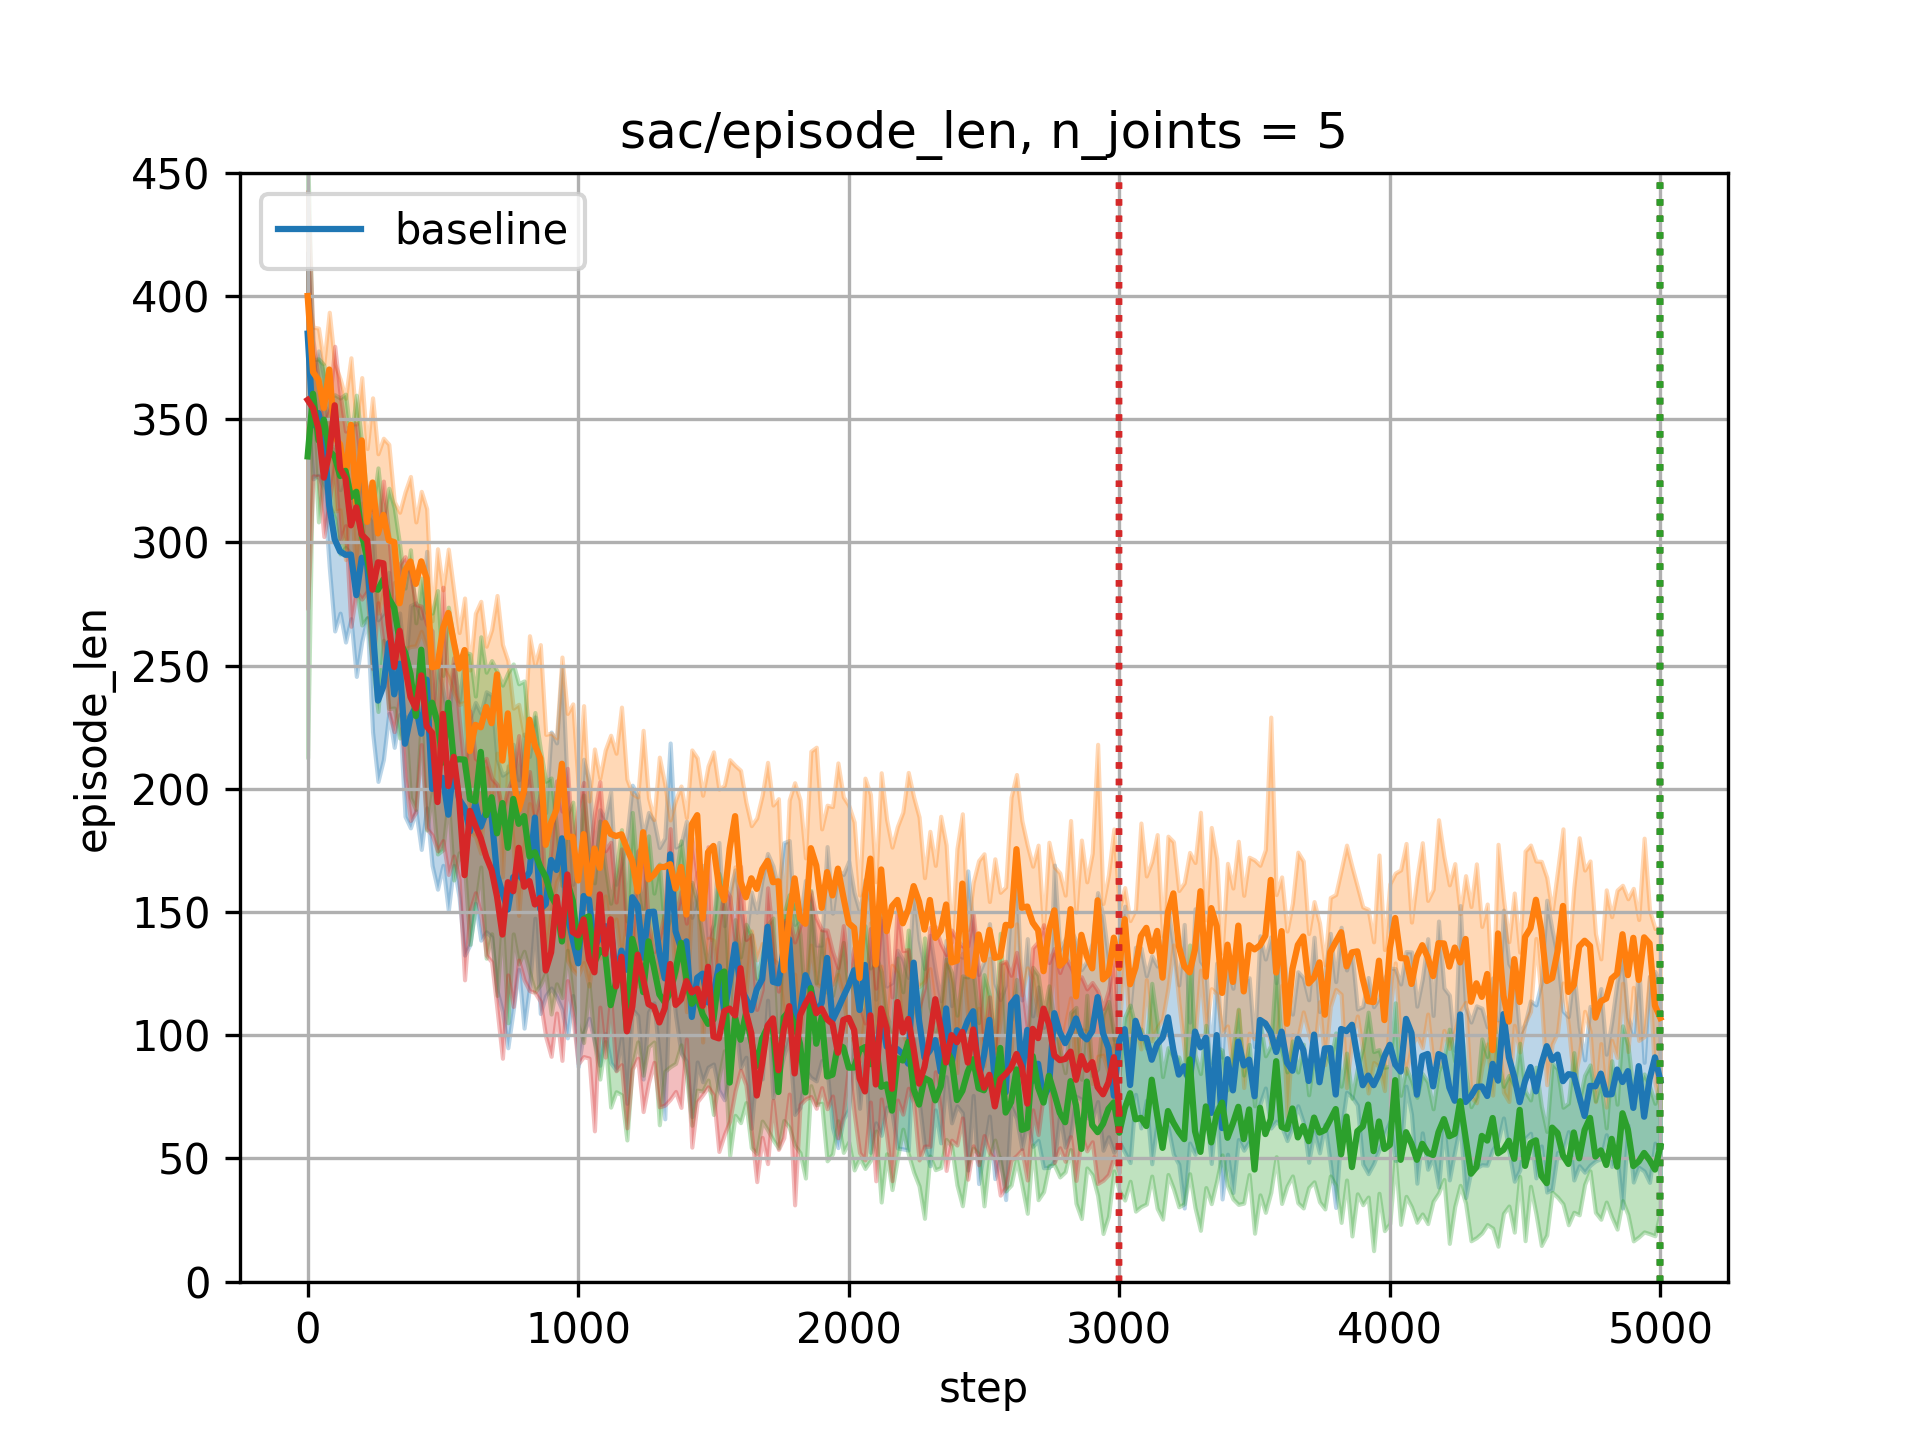
\includegraphics[width=0.23 \linewidth]{figures/experiments/sac_latent_comp_5_vae_episode_len.png}
            \label{fig:SAC_latent_comparison_episode_len/5}
            }
        \hfill    
        \subfloat[$N = 10$]{
            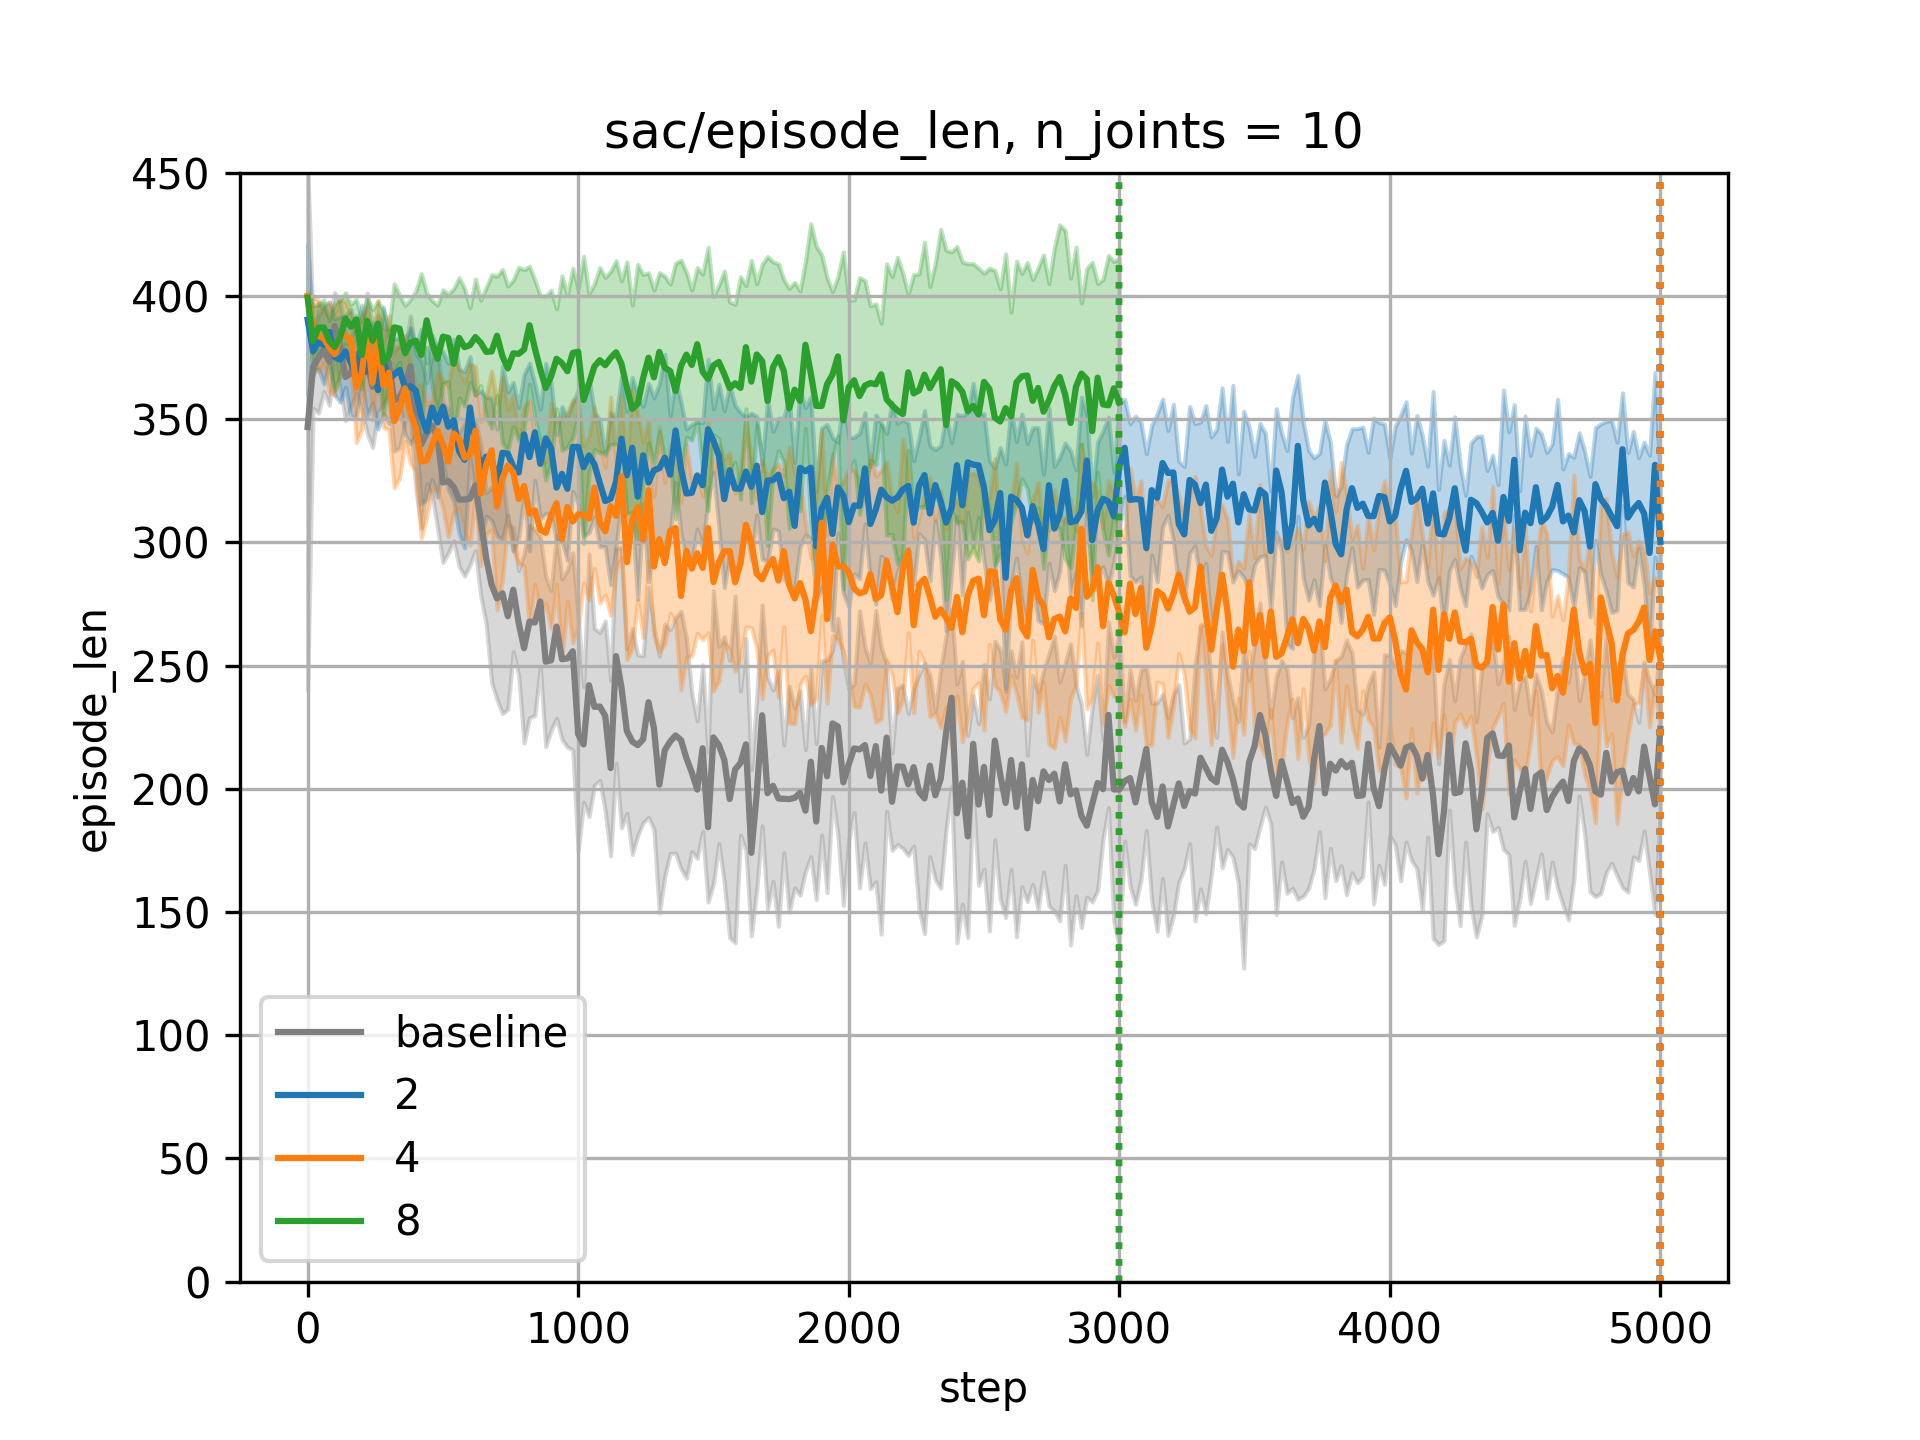
\includegraphics[width=0.23 \linewidth]{figures/experiments/sac_latent_comp_10_vae_episode_len.png}
            \label{fig:SAC_latent_comparison_episode_len/10}
            }
        \hfill
        \subfloat[$N = 15$]{
        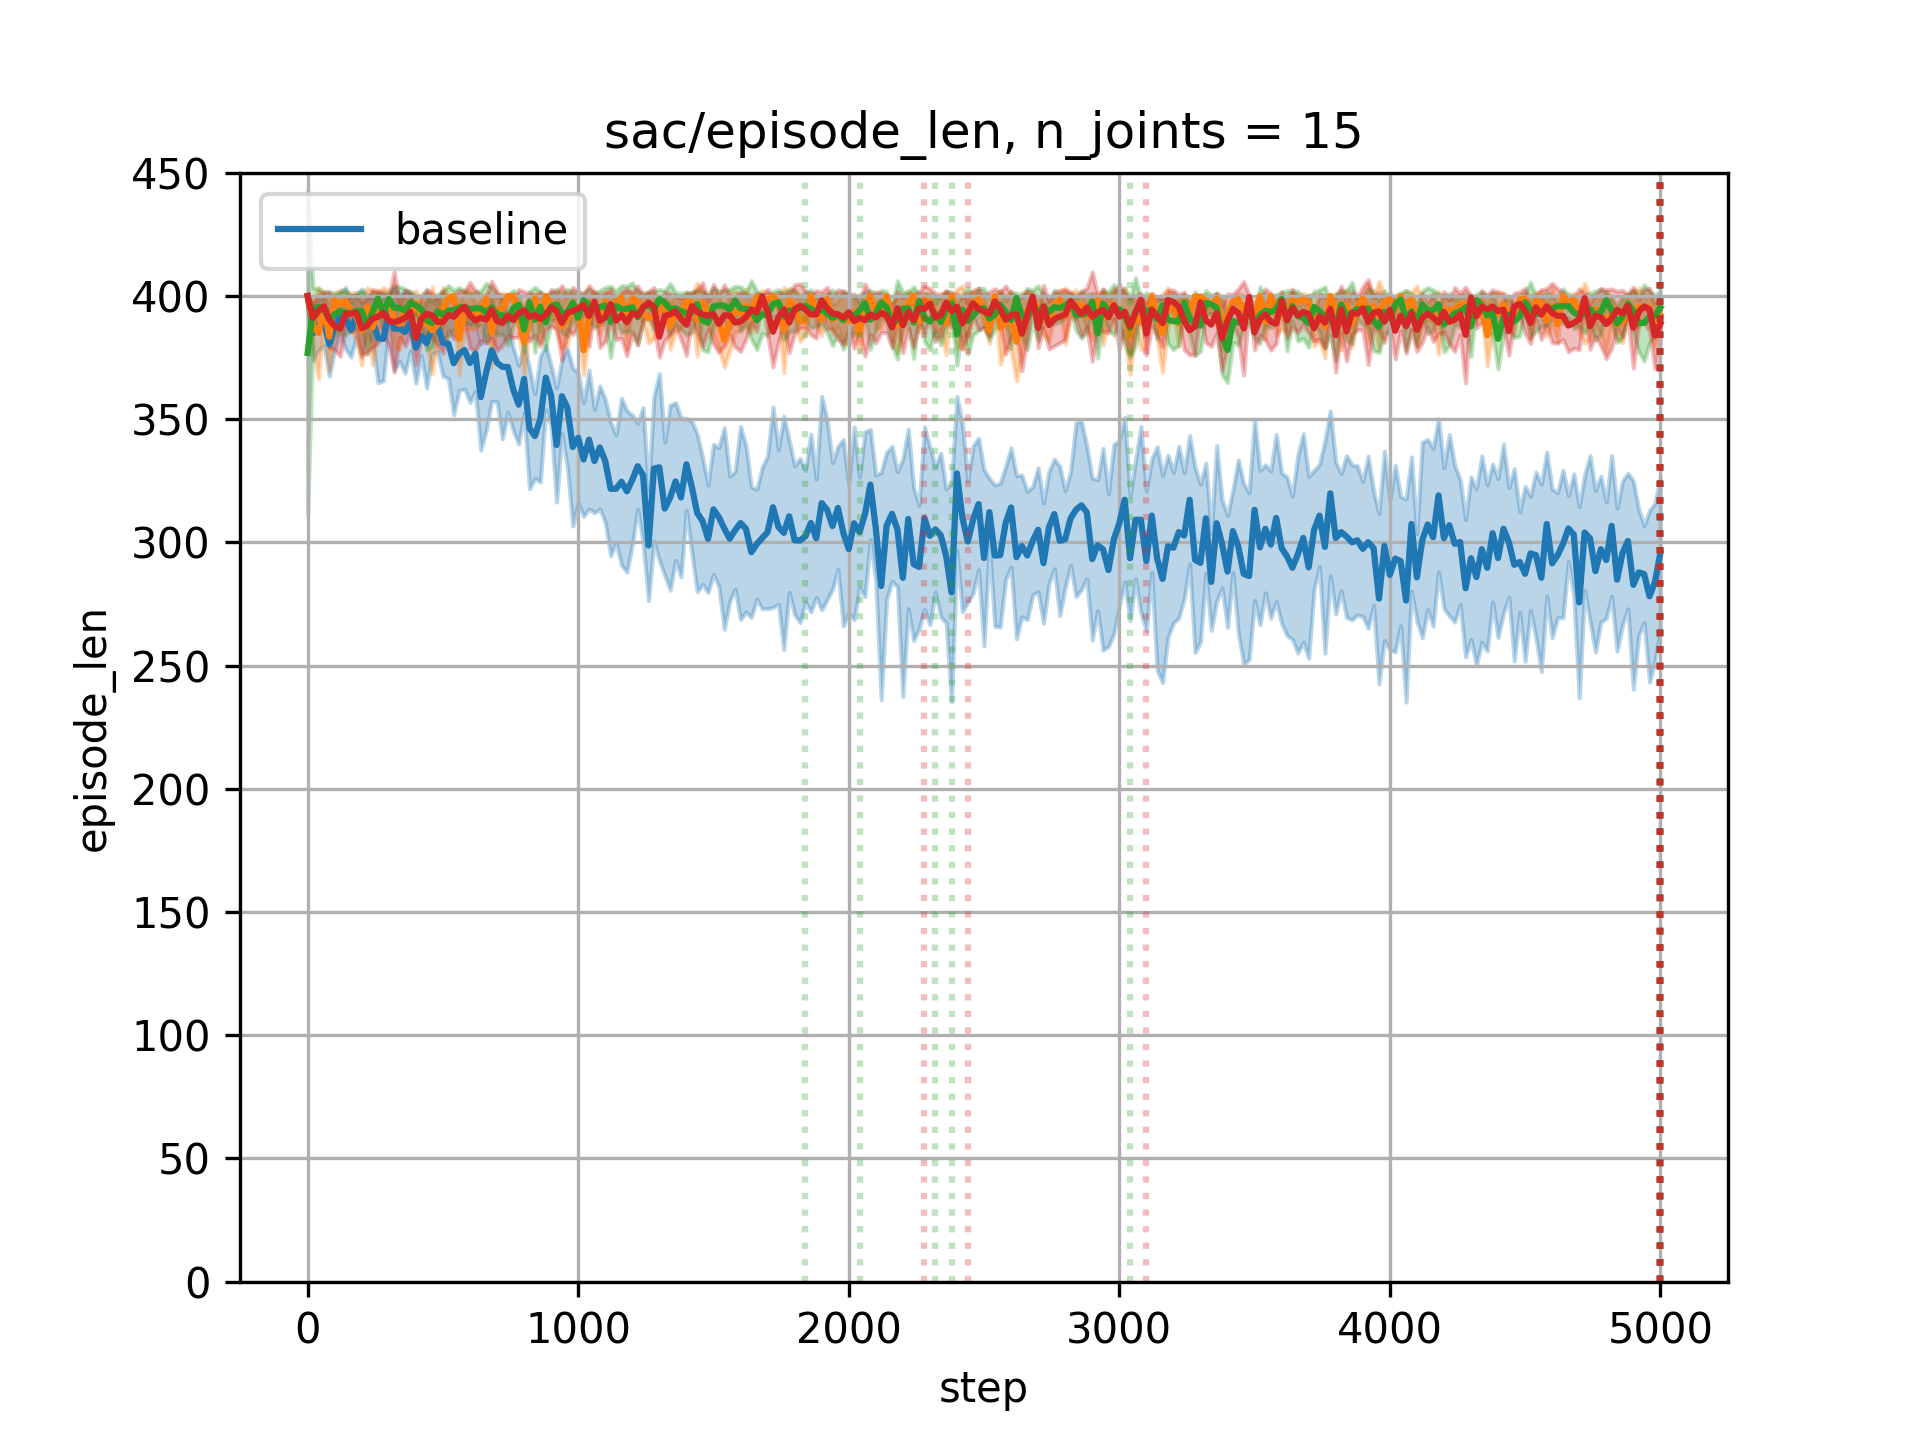
\includegraphics[width=0.23 \linewidth]{figures/experiments/sac_latent_comp_15_vae_episode_len.png}
            \label{fig:SAC_latent_comparison_episode_len/15}
            }
    \end{center}
    \caption[SAC + VAE latent dimension comparison]{Shown are the mean episode length over the the last 20 episodes, compared different latent dimensions and the baseline. Solid line is the mean over 10 experiments and the color shaded area is the corresponding standard deviation. Lower means better with 1 as the minimum and 400 as the maximum.}
    \label{fig:SAC_latent_comparison_episode_len}
\end{figure}

In \figref{fig:SAC_latent_comparison_episode_len} we can observe the mean episode length for different $N \in [2, 5, 10, 15]$. Starting at two joints we can see not much of a difference but at five joints we can observe slight differences between different latent dimensions. First up is the latent dimension of two At this value the experiments perform as in \figref{fig:SAC_latent_comparison_mean_score/5} worst.\\
Moving on to a latent dimension of four, those experiments perform best in terms of mean episode length and even undercut the baseline experiments although they have not performed as good in terms of the mean score per step in \figref{fig:SAC_latent_comparison_mean_score/5}. Finally those experiments with a latent dimension of eight are performing almost on the same level as the baseline experiments but not as good as the experiments with a latent dimension of four. \\
In \figref{fig:SAC_latent_comparison_mean_score/10} we can see wide variety of best performances. The best performing setting are the baseline experiments followed by the experiments with a latent dimension of four. The next best performance is coming from a latent dimension equal to two and last ranked are the experiments with a latent dimension of eight. As we have mentioned earlier we suspect this drop in performance caused by the quality the decoder gets hand over to the Soft Actor Critic. \\
Note that although the maximum number of steps per episode was set to 400 the standard deviation of the experiment with a latent dimension of eight seam to surpass this threshold which is with a closer look into the actual curves clearly not the case. \todo{insert plot in appendix}. \\ 
On the performed experiments with 15 joints we can see that none of the latent experiments is able to match the performance of the baseline experiments with even a couple of experiments with a latent dimension of four or eight aborting early. As it turns out this abort is caused by abnormally high values for alpha loss as shown in \figref{fig:alpha_loss_15} resulting in \texttt{nan} values in update steps. A positive alpha loss translates to a an increase of alpha translates to an increase in exploration for the policy, by encouraging a higher standard deviation for the parameterized distribution returned by the actor network.
\begin{figure}
    \begin{center}
        \subfloat[mean episode reward per step averaged over the last 20 episodes. ]{
            
\includegraphics[width=0.46 \linewidth]{figures/place_holder.png}
            \label{fig:SAC_latent_8/reward}
            }
        \hfill
        \subfloat[mean episode length avergaed over the last 20 episodes]{
        
\includegraphics[width=0.46 \linewidth]{figures/place_holder.png}
            \label{fig:SAC_latent_8/episode_len}
            }
    \end{center}
    \caption[SAC + VAE on latent dim = 4]{SAC + decoder form VAE with \textbf{latent dimension = 4} and trained with imitation loss enabled. Each experiment was conducted 10 times with different random seeds. The solid strong line is the mean over those 10 experiments. The color shaded area covering the mean is the standard deviation around the mean.}
    \label{fig:SAC_latent_8}
\end{figure}

\begin{figure}
    \begin{center}
        \subfloat[SAC baseline experiments]{
            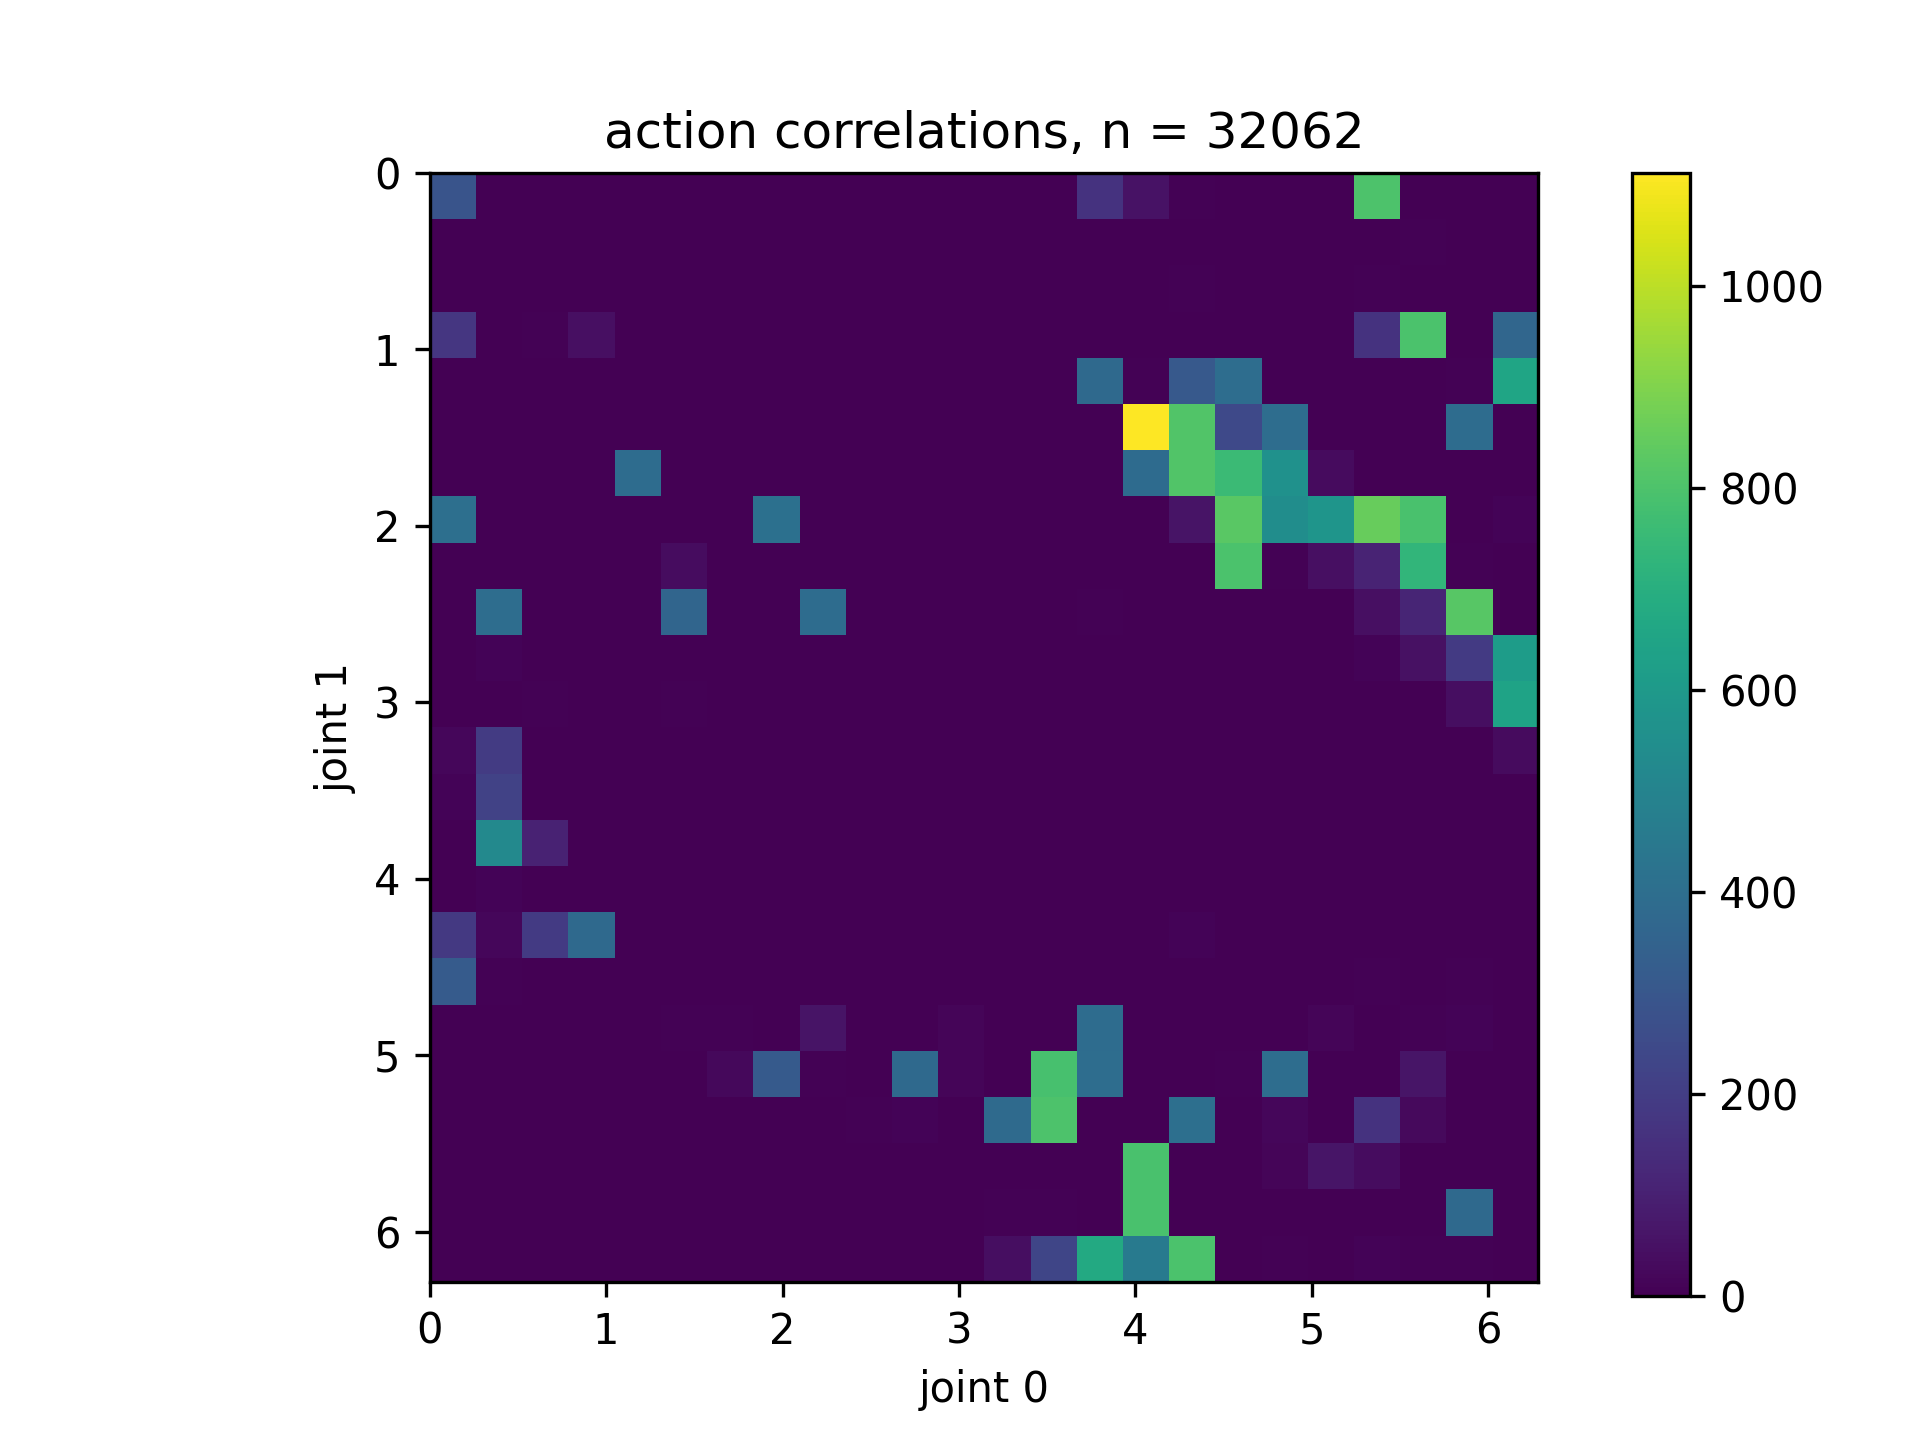
\includegraphics[width=0.31 \linewidth]{figures/experiments/action_correlations_baseline_2_1691621262_5000.png}
            \label{fig:SAC_action_correlation_comp/baseline}
            }
        \hfill
        \subfloat[SAC + VAE with latent dimension = 4 and only distance loss enabled]{
            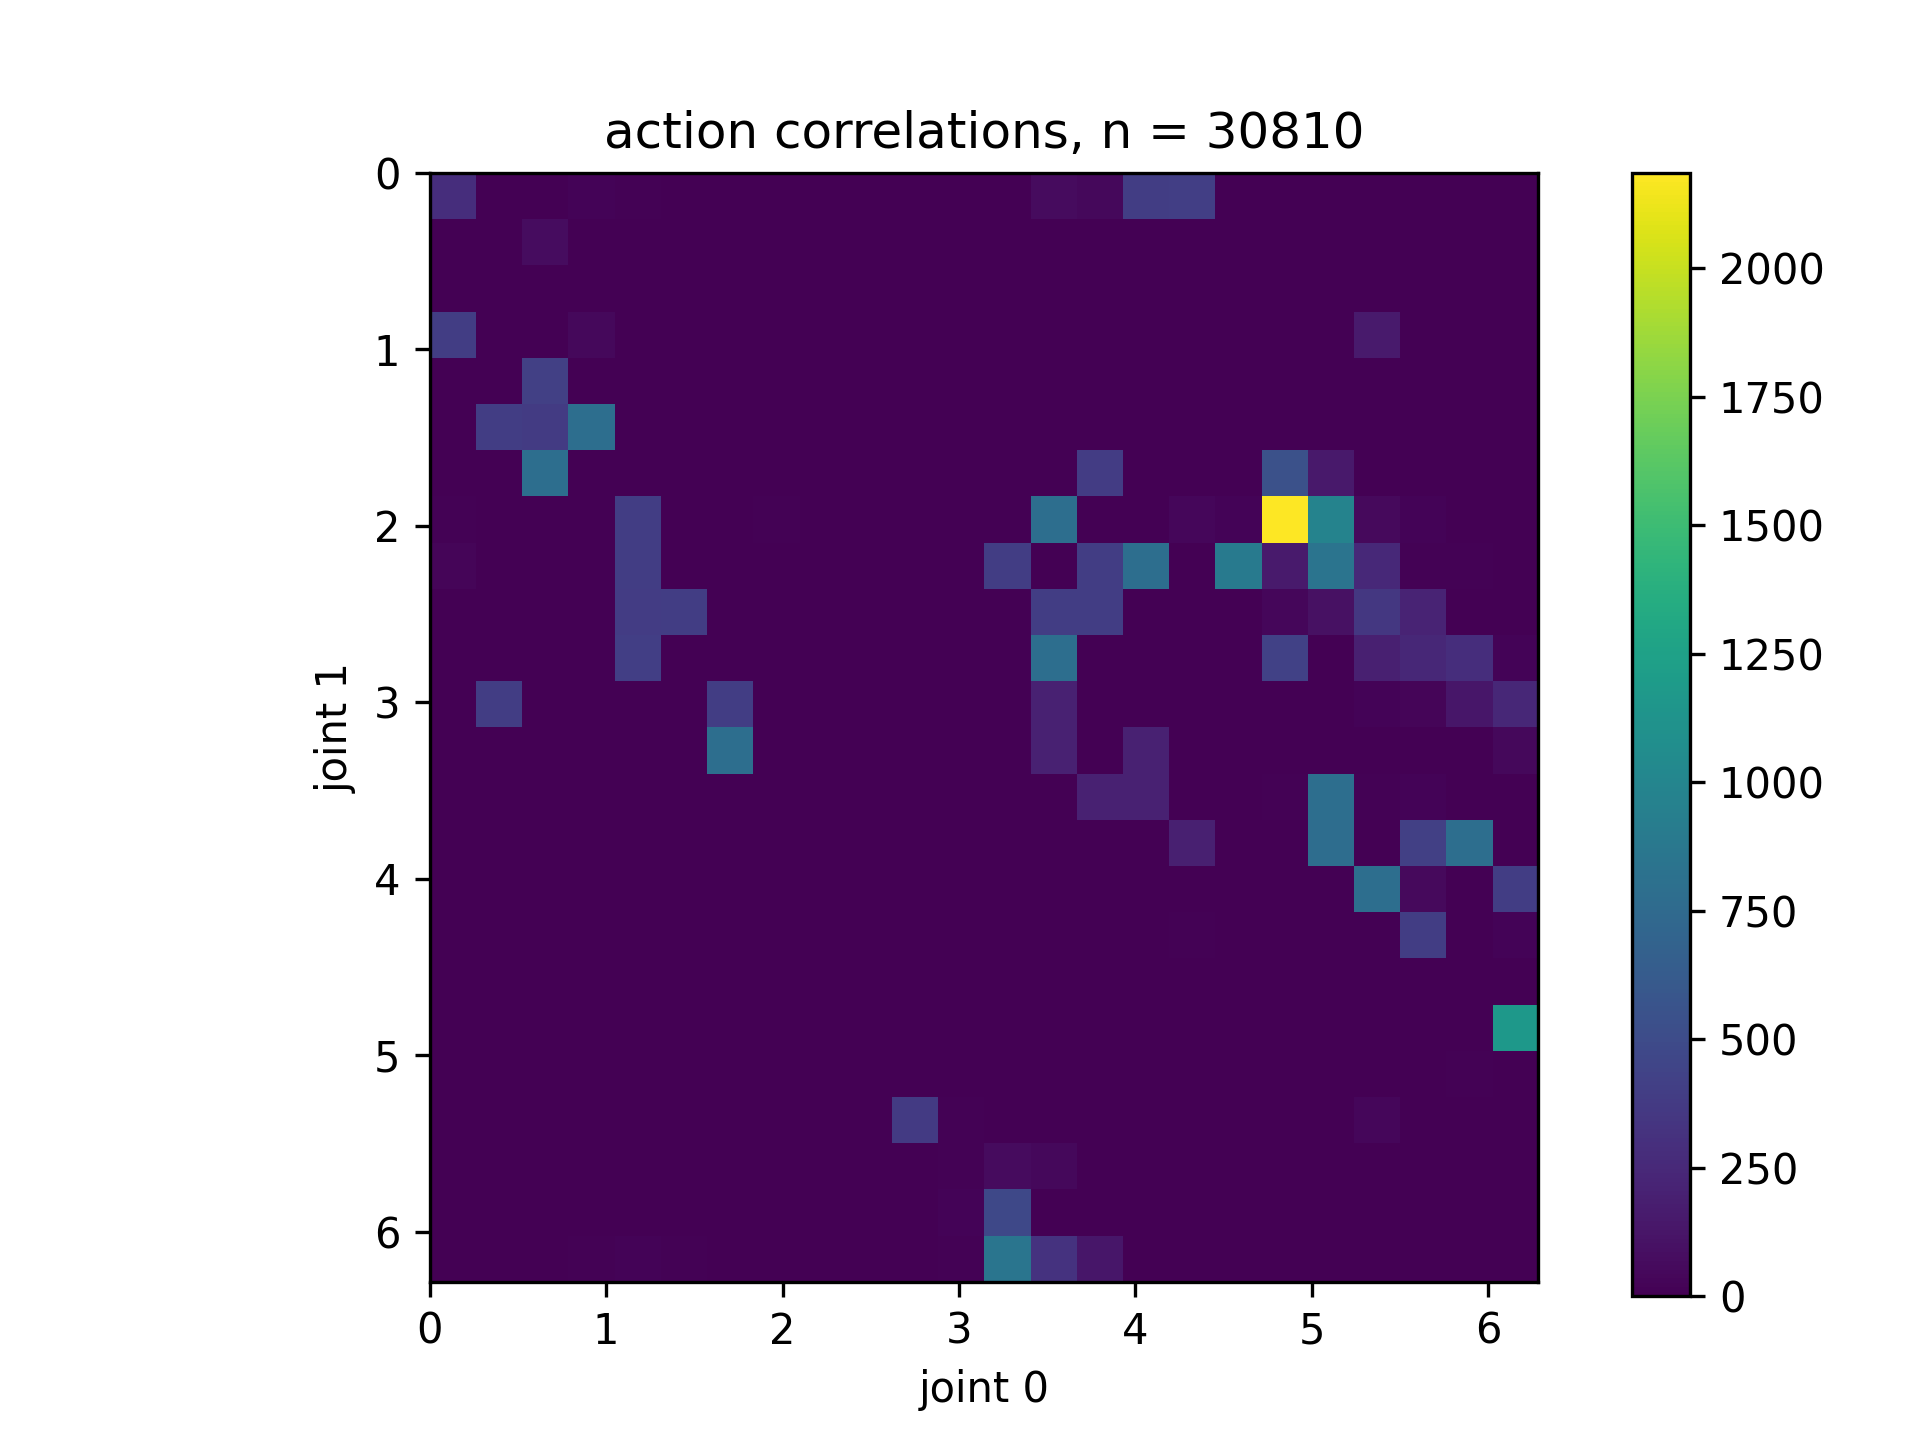
\includegraphics[width=0.31 \linewidth]{figures/experiments/action_correlations_latent_actor_4_2_1693063115_5000.png}
            \label{fig:SAC_action_correlation_comp/latent_4}
            }
        \subfloat[SAC + VAE with latent dimension = 4, distance and imitation loss enabled]{
            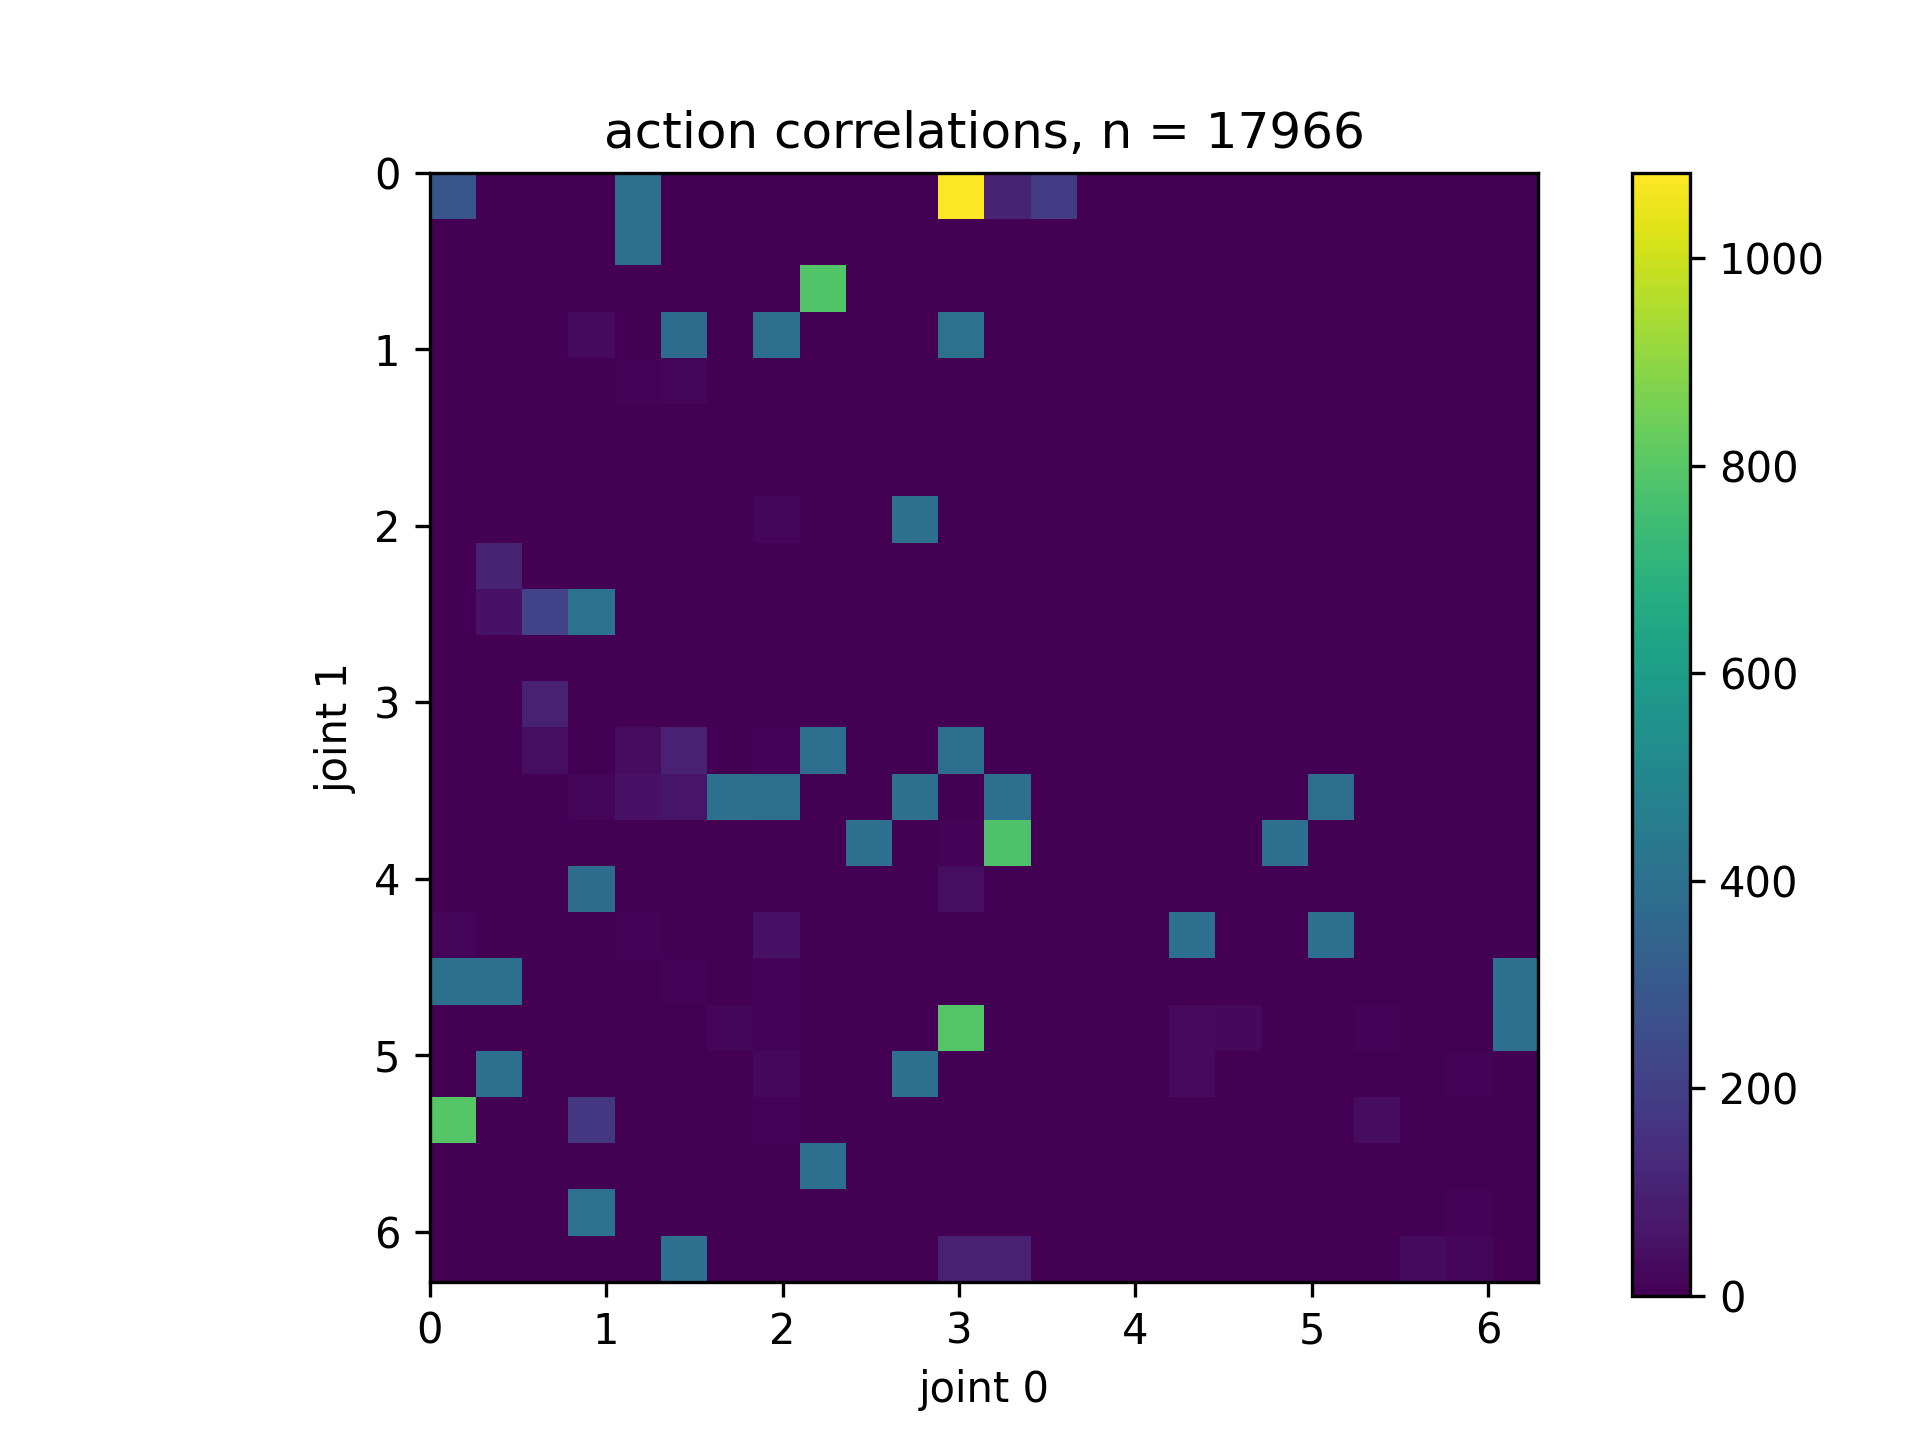
\includegraphics[width=0.31 \linewidth]{figures/experiments/action_correlations_latent_imitation_4_2_1693269830_3000.png}
            \label{fig:SAC_action_correlation_comp/latent_4_imitation}
            }
    \end{center}
    \caption[action correlation comparison]{Action correlation for baseline experiments, latent dimension only trained on distance loss and SAC + VAE trained on distance and imitation loss. }
    \label{fig:SAC_action_correlation_comp}
\end{figure}

Because we have seen a lack in performance between the baseline SAC experiments we additional trained VAEs with the imitation loss enabled to minimize the distance between the state angle distribution the decoder is receiving as in \figref{fig:SAC_action_correlation_comp} versus the state angle distribution the decoder is trained as in \figref{fig:dataset_action_correlation}. But if we have a look into \figref{fig:SAC_action_correlation_comp/latent_4_imitation} and compare to the plots on the left we do not see a significant change. This could be extrapolated to higher $N$ and explain the missing improvement we would expect. But since this is not the main focus of this thesis we leaf these steps for future research.

\subsection{Soft Actor-Critic + Supervised}
\begin{figure}
    \begin{center}
        \subfloat[Mean score per step]{
            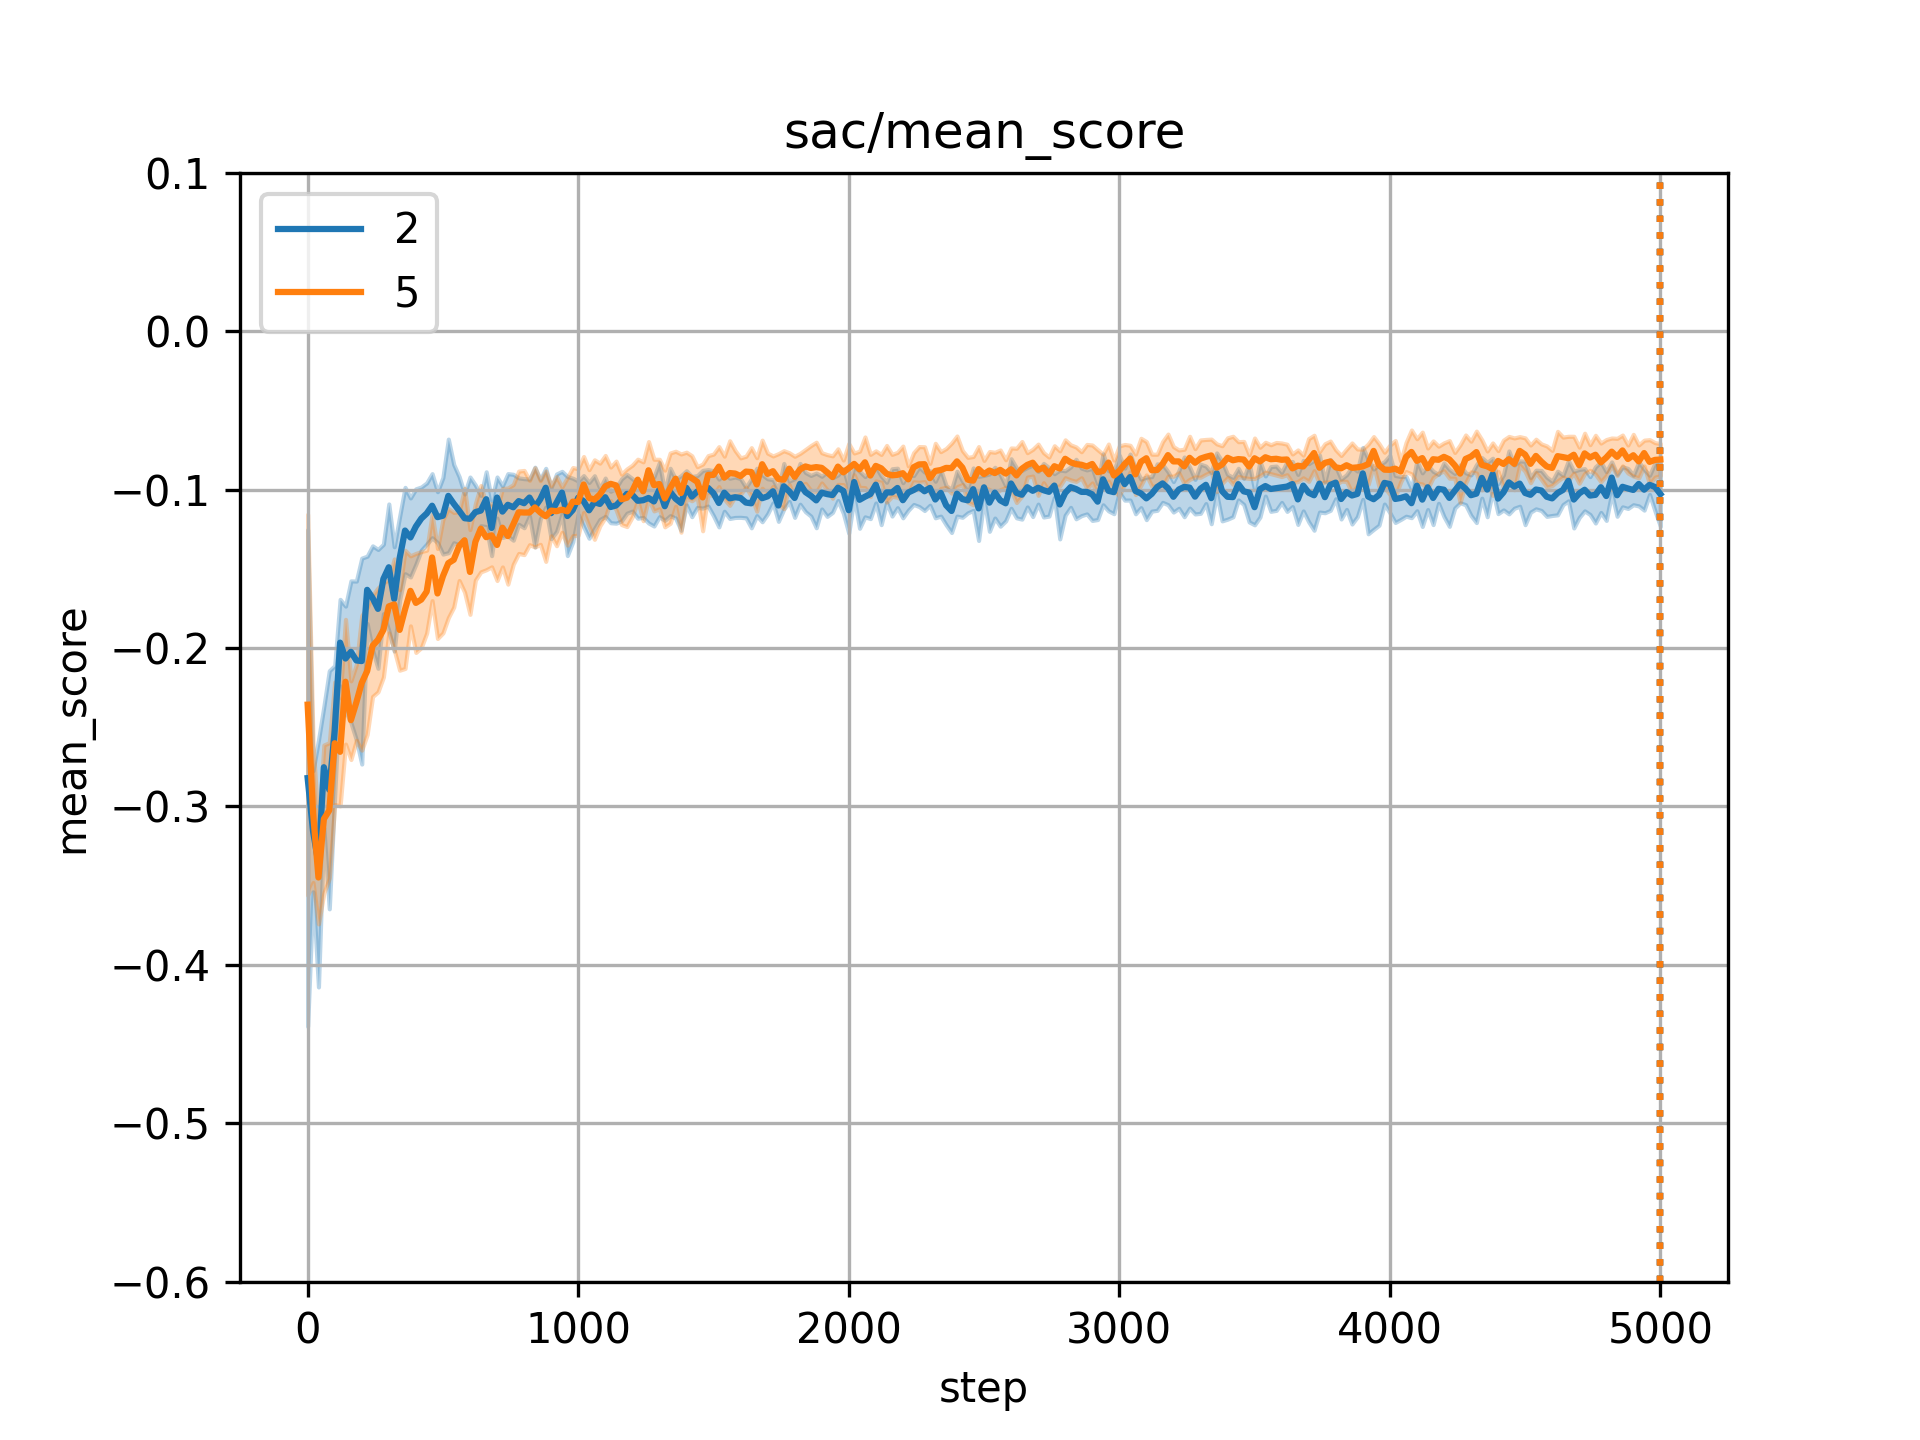
\includegraphics[width=0.46 \linewidth]{figures/experiments/sac_supervised_dist_[2, 5]_mean_score.png}
            \label{fig:sac_supervised/distance_loss}
            }
        \hfill
        \subfloat[episode length]{
        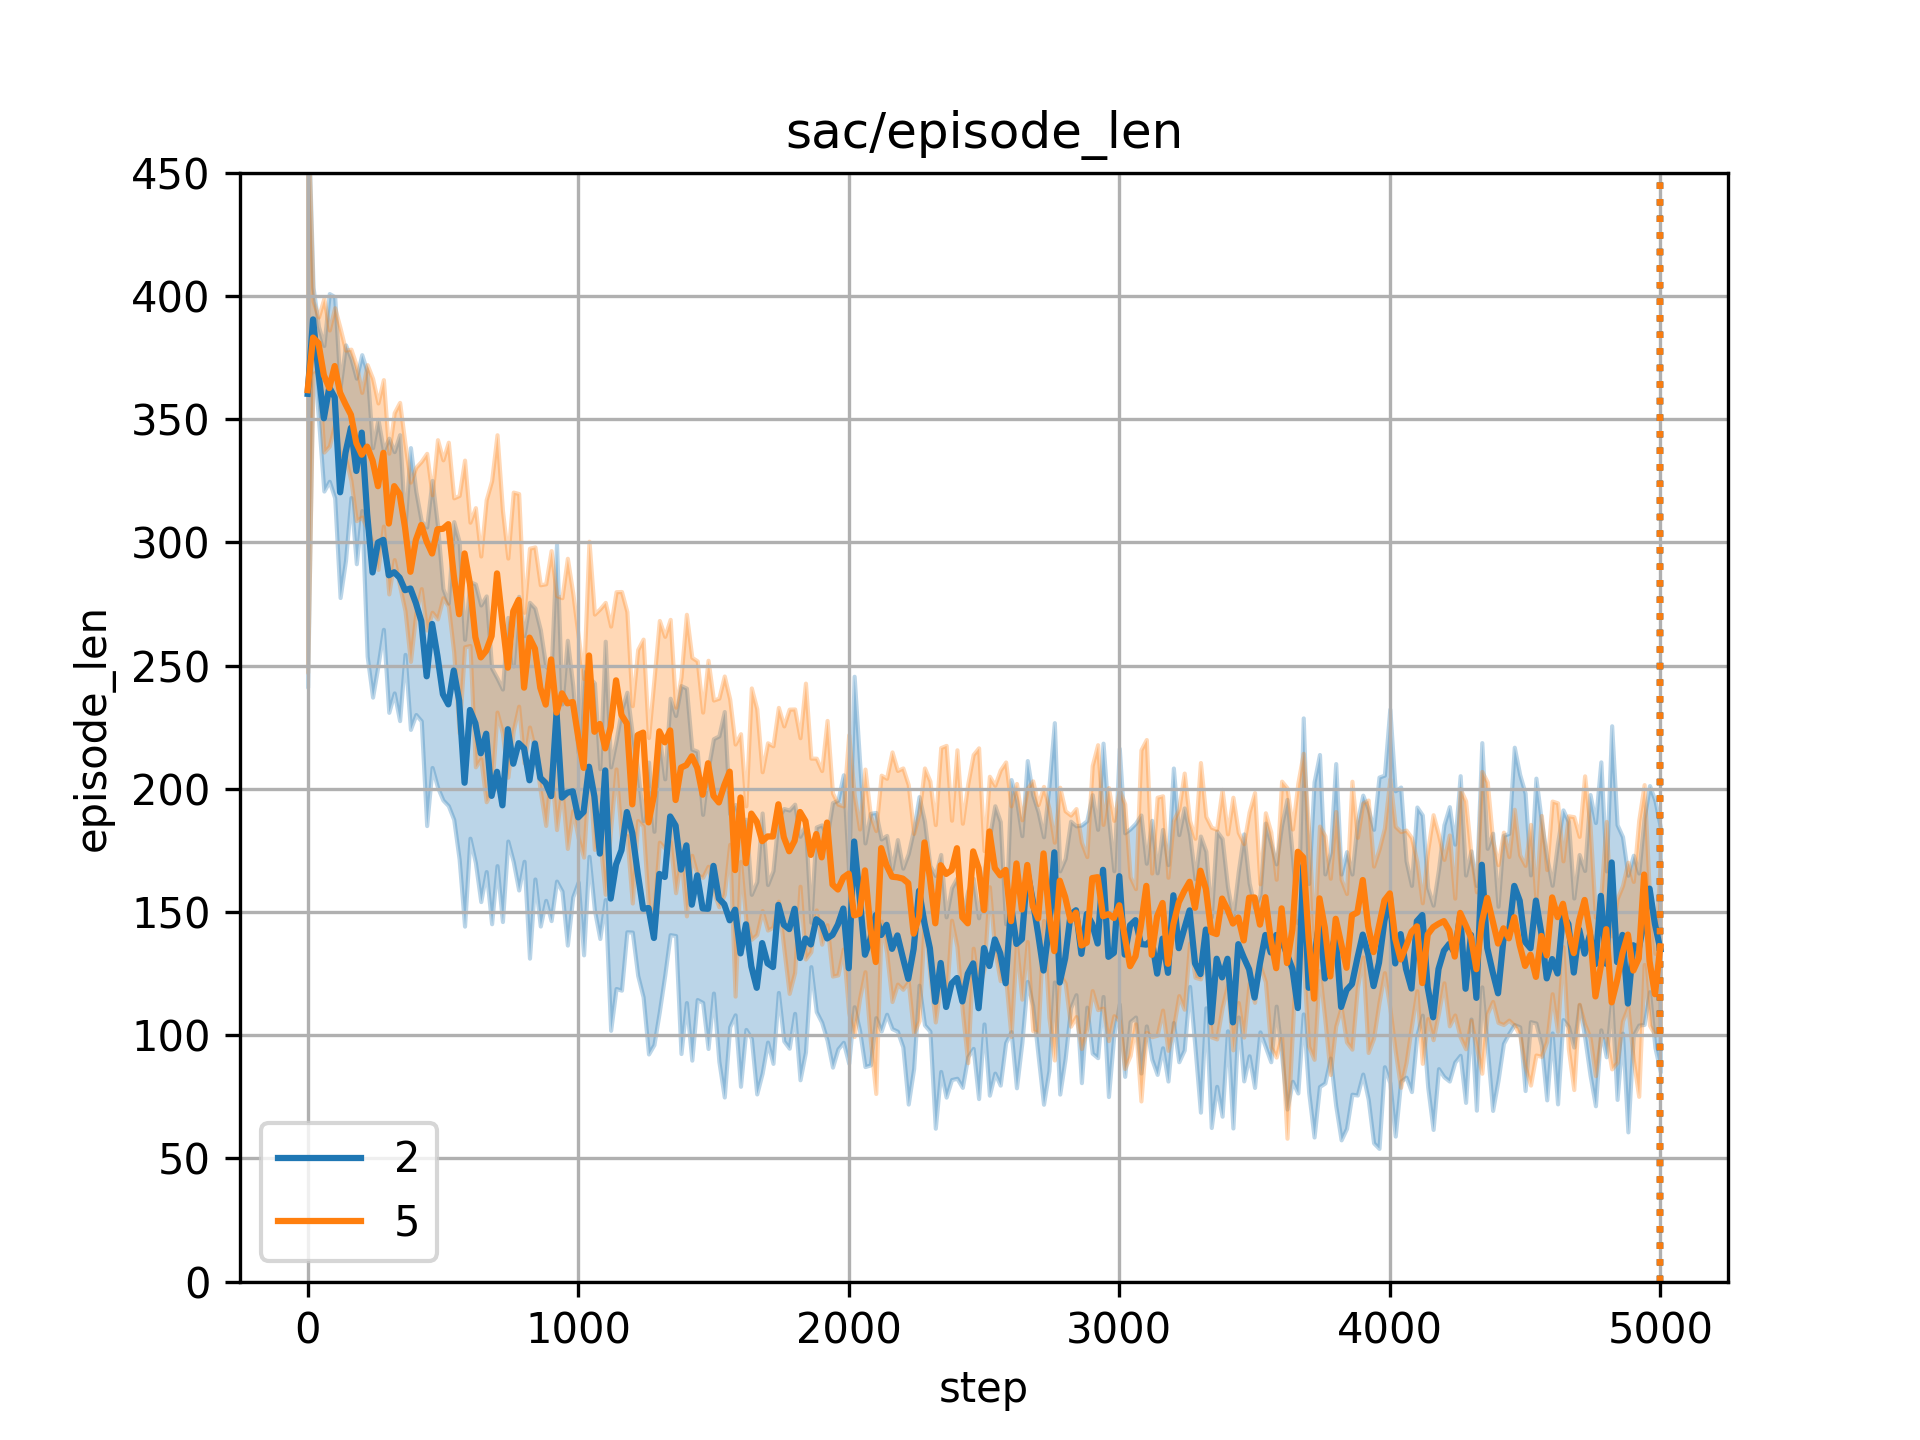
\includegraphics[width=0.46 \linewidth]{figures/experiments/sac_supervised_dist_[2, 5]_episode_len.png}
            \label{fig:sac_supervised/imitation_loss}
            }
    \end{center}
    \caption[Supervised Distance and Imitation Loss]{Validation results for supervised experiments on distance and imitation loss. }
    \label{fig:sac_supervised}
\end{figure}

Merging the supervised model with SAC yields performances as in \figref{fig:sac_supervised}. We do can see very similar performances as with merging SAC with VAE.
\begin{table}
    \begin{center}
        \begin{tabular}{ l | c  c | c  c | c  c}
        experiment series & \multicolumn{6}{c}{$N$} \\
        \hline
        & \multicolumn{2}{c |}{2} & \multicolumn{2}{c |}{5} & \multicolumn{2}{c}{10} \\
        & mean & std. & mean & std. & mean & std. \\
        \hline
        \textit{baseline}                    &  -5.16 & $\pm$ 0.95 & -15.29 & $\pm$ 1.62 & -32.51 & $\pm$ 2.64 \\
        \textit{latent actor 4}              & -13.45 & $\pm$ 2.93 & -15.60 & $\pm$ 2.49 & -15.45 & $\pm$ 4.42\\
        \textit{supervised imitation loss}   &  10.96 & $\pm$ 2.07 &  41.76 & $\pm$ 2.75 &  39.71 & $\pm$ 2.89  \\
        \textit{supervised distance loss}    &  -9.03 & $\pm$ 0.98 & -10.54 & $\pm$ 0.41 & & \\
        \end{tabular}
    \end{center}
    \caption[policy log probabilities]{Log probabilities of each policy series during training form the last 50 episodes each over 10 experiments. }
    \label{tab:policy_log_probs}
\end{table}

A very interesting point of distinguishing the merge of SAC with either the VAE approach or the supervised regressor can be shown by the log probabilities, the actor networks are returning for the gaussian distribution to sample from in \tabref{tab:policy_log_probs}. If we look first at \textit{baseline} the mean log probability decreases with the number of joints and therefor increases the stochastisity of the policy. If we look at the the latent experiments \textit{latent actor 4} and \textit{supervised distance loss} the log probability stays on the same level but is significant higher for the VAE approach. 

\begin{figure}
    \begin{center}
        \subfloat[Mean score per step]{
            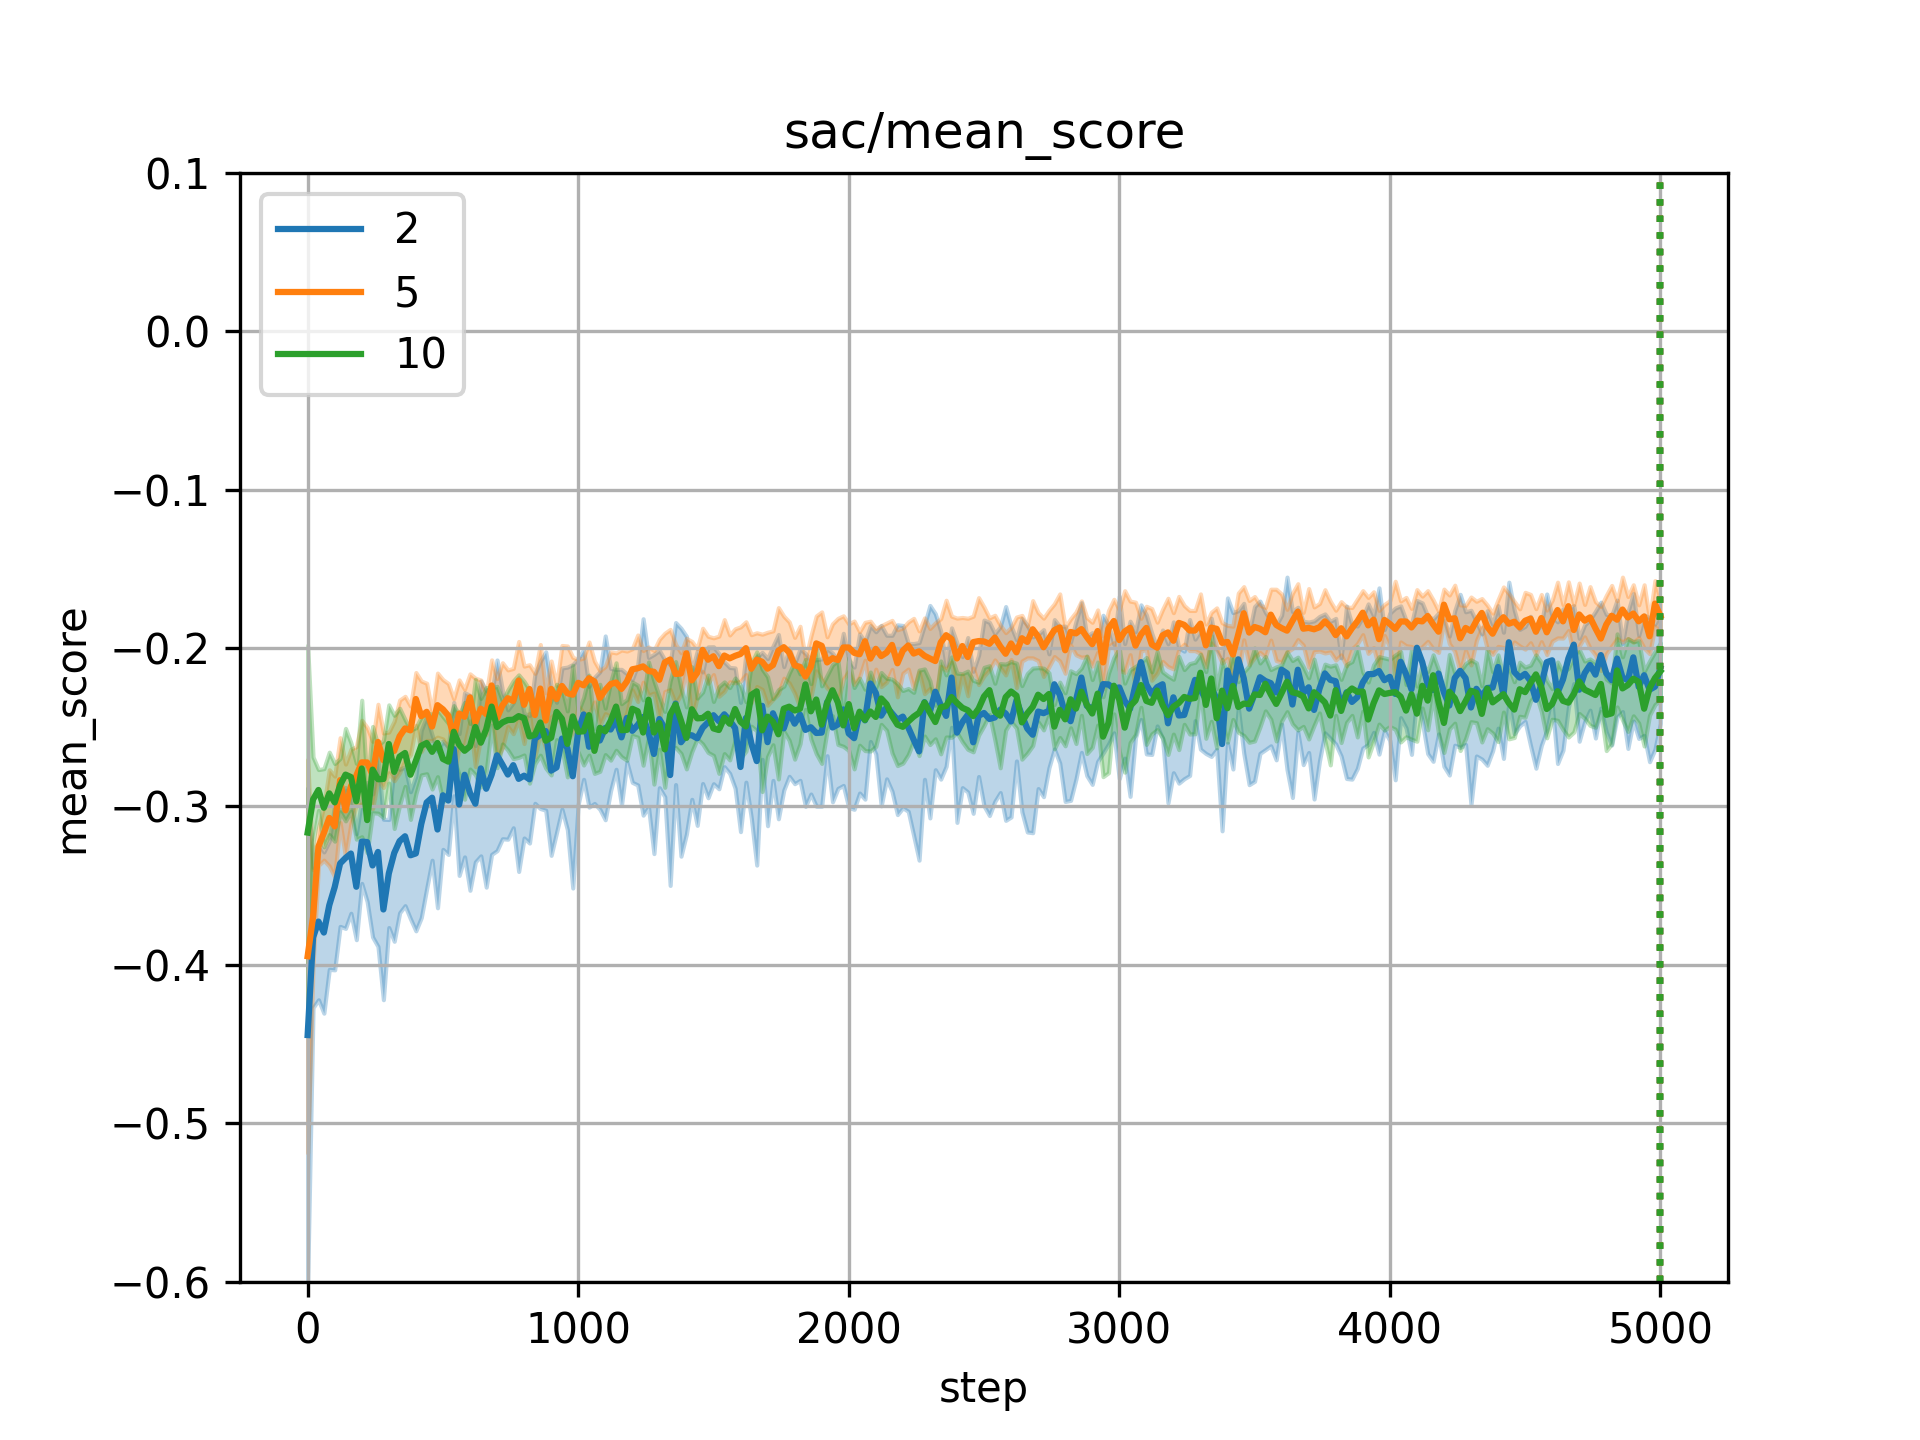
\includegraphics[width=0.46 \linewidth]{figures/experiments/sac_supervised_imitation[2, 5, 10]_mean_score.png}
            \label{fig:sac_supervised_imitation/distance_loss}
            }
        \hfill
        \subfloat[episode length]{
        \includegraphics[width=0.46 \linewidth]{figures/experiments/sac_supervised_imitation[2, 5, 10]_episode_len.png}
            \label{fig:sac_supervised_imitation/imitation_loss}
            }
    \end{center}
    \caption[Supervised Distance and Imitation Loss]{Validation results for supervised experiments on distance and imitation loss. }
    \label{fig:sac_supervised_imitation}
\end{figure}

Experiments conducted with a supervised model trained with imitation loss enabled are shown in \figref{fig:sac_supervised_imitation}.

A further property is the log probability the imitation loss regressor experiments are returning during training as in \tabref{tab:policy_log_probs}. The actor network is very certain about the action it would like to exploit leaving almost no room for exploration. 

\begin{figure}
    \begin{center}
        \subfloat[SAC baseline experiments]{
            \includegraphics[width=0.31 \linewidth]{figures/experiments/action_correlations_baseline_2_1691621262_5000.png}
            \label{fig:SAC_action_correlation_supervised/baseline}
            }
        \hfill
        \subfloat[SAC + Supervised model trained only with distance loss enabled]{
            \includegraphics[width=0.31 \linewidth]{figures/experiments/action_correlations_supervised_dist_loss_2_1693272467_3000.png}
            \label{fig:SAC_action_correlation_supervised/supervised}
            }
        \subfloat[SAC + Supervised model trained only with distance loss enabled]{
            \includegraphics[width=0.31 \linewidth]{figures/place_holder.png}
            \label{fig:SAC_action_correlation_supervised/supervised_imitation}
            }
    \end{center}
    \caption[action correlation comparison with supervised model]{Action correlation for baseline experiments, experiments with SAC and supervised model with only distance loss enabled and SAC with supervised model with distance and imitation loss enabled.}
    \label{fig:SAC_action_correlation_supervised}
\end{figure}
